\documentclass[11pt,a4paper]{ctexart}
\usepackage[margin=2cm]{geometry}
\usepackage{listings}
\usepackage{amsmath}
\usepackage{xcolor}
\usepackage{hyperref}
\usepackage{pdfpages}
\hypersetup{colorlinks=true,linkcolor=black,urlcolor=blue}
\lstset{
  language=C++,
  basicstyle=\ttfamily\scriptsize,
  keywordstyle=\color{blue!70!black}\bfseries,
  commentstyle=\color{green!45!black},
  stringstyle=\color{red!60!black},
  numbers=left, numberstyle=\tiny\color{gray}, numbersep=6pt,
  frame=single, framexleftmargin=10pt,
  breaklines=true, breakatwhitespace=false,
  keepspaces=true, tabsize=4, columns=fullflexible,
  showstringspaces=false, extendedchars=true,
  xleftmargin=14pt
}
\begin{document}
\title{板子库}
\author{mortal \& hecc}
\date{}
\maketitle
\tableofcontents
\newpage

\section{dp}

\subsection{单调队列优化}

\begin{lstlisting}
// 原题：琪露诺

dp[0] = 0;
	for (int i = l; i <= n; i++)
	{
		while (!p.empty() && dp[p.back()] <= dp[i - l])
			p.pop_back();
		while (!p.empty() && p.front() < i - r)
			p.pop_front();
		p.push_back(i - l);
		dp[i] = dp[p.front()] + a[i];
		if (i + r > n)
			ans = max(ans, dp[i]);
	}
\end{lstlisting}

\subsection{数位dp基本过程}

\begin{lstlisting}
#include<bits/stdc++.h>
using namespace std;
#define int long long

int a, b;
int num[25], cnt;
int dp[25][5][5][15];

int dfs(int site, bool limit, bool first, int dig)
{
    // site -> 考虑到第 site 位
    // limit -> 是否顶到上界
    // first -> 是否开始填数
    // dig -> 上一位的数码是多少
    if (!site)
        return first; // 开始填数了才有 1 种方案
    if (dp[site][limit][first][dig] != -1)
        return dp[site][limit][first][dig];
    
    int res = 0;
    int up = limit ? num[site] : 9;

    for (int i = 0; i <= up; i++)
    {
        bool newlimit = limit && (i == up);
        bool newfirst = first || i;
        if (!first) // 没开始填数，这个填什么都行
            res += dfs(site - 1, newlimit, newfirst, i);
        else // 开始填数了，必须满足 （某些限制条件）|i - dig| >= 2
        {
            if (abs(i - dig) < 2) continue;
            res += dfs(site - 1, newlimit, newfirst, i);
        }
    }

    return dp[site][limit][first][dig] = res;
}

int solve(int x)
{
    cnt = 0;
    while (x)
    {
        num[++cnt] = x % 10;
        x /= 10;
    }
    memset(dp, -1, sizeof(dp));
    return dfs(cnt, 1, 0, 0);
}

signed main()
{
    cin >> a >> b;
    cout << solve(b) - solve(a - 1);
    return 0;
}
\end{lstlisting}

\subsection{斜率优化}

\begin{lstlisting}
// 一定要注意斜率的判断方向，是上凸还是下凸，维护max还是min


// x, k 都是单调
#include<bits/stdc++.h>
using namespace std;
#define int long long

const int maxn = 1e6 + 10;
int n;
int a, b, c;
int sum[maxn], dp[maxn];
int q[maxn], l = 0, r = 0;

int X(int id)
{
	return sum[id];
}

int Y(int id)
{
	return dp[id] + a * sum[id] * sum[id] - b * sum[id];
}

double solpe(int x, int y, int X, int Y)
{
	if (x == X)
		return (Y > y) ? 1e18 : -1e18;
	return (1.0 * (Y - y)) / (1.0 * (X - x));
}

signed main()
{
	cin >> n >> a >> b >> c;
	for (int i = 1; i <= n; i++)
		cin >> sum[i], sum[i] += sum[i - 1];
	dp[1] = a * sum[1] * sum[1] + b * sum[1] + c;
	q[++r] = 1;

	for (int i = 2; i <= n; i++)
	{
		int k = 2 * a * sum[i];
		while (l < r && solpe(X(q[l]), Y(q[l]), X(q[l + 1]), Y(q[l + 1])) >= k)
			l++;
		int j = q[l];
		dp[i] = dp[j] + a * (sum[i] - sum[j]) * (sum[i] - sum[j]) + b * (sum[i] - sum[j]) + c;
		while (l < r && solpe(X(q[r - 1]), Y(q[r - 1]), X(q[r]), Y(q[r])) <= solpe(X(q[r]), Y(q[r]), X(i), Y(i)))
			r--;
		q[++r] = i;
	}
	cout << dp[n];
	return 0;
}

// x 单调，k 不单调，做单调队列上二分，凸壳正常维护即可

// xk都不单调，考虑 cdq 分治或者李超线段树
// cdq 分治：
#include<bits/stdc++.h>
using namespace std;
#define int long long

const int maxn = 1e5 + 10;
int n;
int  h[maxn], sum[maxn];
int dp[maxn];
struct Query{
    int x, y, id;
}q[maxn];
int que[maxn];

double slope(int x, int y, int X, int Y)
{
    if (x == X)
        return -1e18;
    return (1.0 * (Y - y)) / (1.0 * (X - x));
}

int X(int id)
{
    return h[id];
}

int Y(int id)
{
    return dp[id] - sum[id] + h[id] * h[id];
}

bool cmpx(Query a, Query b)
{
    if (a.x == b.x)
        return a.y > b.y;
    return a.x < b.x;
}

bool cmpk(Query a, Query b)
{
    return h[a.id] < h[b.id];
}

bool cmpid(Query a, Query b)
{
    return a.id < b.id;
}

void cdq(int L, int R)
{
    if (L == R)
    {
        q[L].x = X(q[L].id);
        q[L].y = Y(q[L].id);
        return ;
    }
    int mid = (L + R) >> 1;
    cdq(L, mid);

    int l = 1, r = 0;
    // 这里左边 x 有序，我们先维护左边的一个下凸壳，用左边的凸壳去求右边的答案
    for (int i = L; i <= mid; i++)
    {
        while (l < r && slope(q[que[r]].x, q[que[r]].y, q[que[r - 1]].x, q[que[r - 1]].y) >= slope(q[i].x, q[i].y, q[que[r]].x, q[que[r]].y))
            r--;
        que[++r] = i;
    }

    // 右边要 k 递增
    sort(q + mid + 1, q + R + 1, cmpk);
    // 然后求右边的答案
    for (int i = mid + 1; i <= R; i++)
    {
        while (l < r && slope(q[que[l]].x, q[que[l]].y, q[que[l + 1]].x, q[que[l + 1]].y) <= 2 * h[q[i].id])
            l++;
        int j = que[l];
        dp[q[i].id] = min(dp[q[i].id], dp[q[j].id] + (h[q[i].id] - h[q[j].id]) * (h[q[i].id] - h[q[j].id]) + sum[q[i].id - 1] - sum[q[j].id]);
    }
    // 重新回到初始状态
    sort(q + mid + 1, q + R + 1, cmpid);
    cdq(mid + 1, R);
    // 保证上面的区间的左边 x 有序
    sort(q + L, q + R + 1, cmpx);
}

signed main()
{
    memset(dp, 0x3f, sizeof dp);
    dp[1] = 0;
    cin >> n;
    for (int i = 1; i <= n; i++)
        cin >> h[i], q[i].id = i;
    for (int i = 1; i <= n; i++)
        cin >> sum[i], sum[i] += sum[i - 1];
    cdq(1, n);
    cout << dp[n];
    return 0;
}
\end{lstlisting}

\subsection{前缀和优化}

\begin{lstlisting}
原题：求n的排列中有多少个排列恰好有k个逆序对
转移：dp_{i,j}=dp_{i-1,j}+...+dp_{i-1}{j-i+1}

#include<bits/stdc++.h>
using namespace std;

int n, k;
int dp[1010][1010];// 在 1-i 的排列中，逆序对数为 j 的方案数
const int mod = 10000;

int main() {
	scanf("%d%d", &n, &k);
	dp[1][0] = 1;
	for (int i = 2; i <= n; i++) {
		int sum = 0;
		for (int j = 0; j <= k; j++) {
			sum = (sum + dp[i - 1][j]) % mod;
			dp[i][j] = sum;
			if (j >= i - 1)
				sum = (sum + mod - dp[i - 1][j - i + 1]) % mod;
		}
	}
	cout << dp[n][k];
}
\end{lstlisting}

\subsection{状压dp}

\begin{lstlisting}
原题：互不侵犯（8连通块内不能有其他棋子）

#include<bits/stdc++.h>
using namespace std;
#define ll long long
int n, K;
ll dp[15][1026][210], ans;
int nn, i, j, k, l, L;

int get(ll x) {
	int res = 0;
	while (x) {
		if (x & 1) res++;
		x >>= 1;
	}
	return res;
}
bool check(int x, int y) {
	// 判断相邻两行是否合法
	if ((y >> 1)&y)return 1;
	if (x & y) return 1;
	if ((x << 1)&y) return 1;
	if ((x >> 1)&y) return 1;
	return 0;
}

int main() {
	scanf("%d%d", &n, &K);
	dp[0][0][0] = 1;
	nn = (1 << n) - 1;
	for (i = 1; i <= n; i++) { //枚举每一行
		for (j = 0; j <= K; j++) {
			for (k = 0; k <= nn; k++) { // 枚举每一种状态
				L = get(k);
				if (L > j) continue;
				if ((k >> 1)&k) continue; // 本行不合法
				for (l = 0; l <= nn; l++) { // 上一行的状态
					if (check(l, k)) continue;
					dp[i][k][j] += dp[(i - 1) ][l][j - L];
				}
			}

		}
	}
	for (i = 0; i <= nn; i++)
		ans += dp[n][i][K];
	cout << ans;
	return 0;
}
\end{lstlisting}

\subsection{线段树优化}

\begin{lstlisting}
原题：最长公共子序列（本质转化成最长上升子序列）

#include<bits/stdc++.h>
using namespace std;

const int maxn = 1e5 + 10;
int n;
int p1[maxn], p2[maxn];
int a[maxn];
int t[maxn];
int ans;
int dp[maxn];

struct Segment{
    int var[maxn << 2];

    void pushup(int p)
    {
        var[p] = max(var[p << 1], var[p << 1 | 1]);
    }

    void change(int p, int l, int r, int pos, int x)
    {
        if (l == r)
        {
            var[p] = max(var[p], x);
            return ;
        }
        int mid = (l + r) >> 1;
        if (pos <= mid) change(p << 1, l, mid, pos, x);
        else change(p << 1 | 1, mid + 1, r, pos, x);
        pushup(p);
    }

    int query(int p, int l, int r, int L, int R)
    {
        if (L <= l && r <= R)
            return var[p];
        int res = 0;
        int mid = (l + r) >> 1;
        if (L <= mid) res = max(res, query(p << 1, l, mid, L, R));
        if (mid < R) res = max(res, query(p << 1 | 1, mid + 1, r, L, R));
        return res;
    }
}T;

int main()
{
	cin >> n;
	for(int i = 1; i <= n; i++)
		cin >> p1[i];
	for(int i = 1; i <= n; i++)
		cin >> p2[i], a[p2[i]] = i;
	for(int i = 1; i <= n; i++)
		p1[i] = a[p1[i]];
    // 等价于求 p1 的最长上升子序列
	for(int i = 1; i <= n; i++)
	{
		dp[i] = T.query(1, 1, n, 1, p1[i]) + 1;
		T.change(1, 1, n, p1[i], dp[i]);
		ans = max(ans, dp[i]);
	}
	cout << ans;
	return 0;
}
\end{lstlisting}

\section{图论}

\subsection{2-SAT问题}

\begin{lstlisting}
#include <bits/stdc++.h>
using namespace std;
int n,m,tot,ver[5000010],hed[5000010],nxt[5000010],blg[5000010];
int low[5000010],dfn[5000010],cnt,ins[5000010],smscc;
stack<int> s;
void tarjan(int u){
	low[u]=dfn[u]=++cnt;
	ins[u]=1;
	s.push(u);
	for(int i=hed[u];i;i=nxt[i]){
		int v=ver[i];
		if(!dfn[v]){
			tarjan(v);
			low[u]=min(low[u],low[v]);
		}
		else if(ins[v]){
			low[u]=min(low[u],dfn[v]);
		}
	}
	if(dfn[u]==low[u]){
		int k=0;
		smscc++;
		do{
			k=s.top();
			s.pop();
			blg[k]=smscc;
			ins[k]=0;
		}while(k!=u);
	}
}
void add(int a,int b){
	ver[++tot]=b,nxt[tot]=hed[a],hed[a]=tot;
}
int main(){
    cin>>n>>m;
    for(int i=1;i<=m;i++){
		int a,ca,b,cb;
		cin>>a>>ca>>b>>cb;
		add(a+(ca^1)*n,b+cb*n);
		add(b+(cb^1)*n,a+ca*n);	
	}
	for(int i=1;i<=n*2;i++){
		if(!dfn[i]){
			tarjan(i);
		}
	}
	for(int i=1;i<=n;i++){
		if(blg[i]==blg[i+n]){
			cout<<"IMPOSSIBLE";
			return 0;
		}
	}
	cout<<"POSSIBLE"<<endl;
	for(int i=1;i<=n;i++){
		cout<<(blg[i]>blg[i+n])<<" ";
	}
    return 0;
}
/*
有 n 个布尔变量 x ，另有 m 个需要满足的条件，
每个条件的形式都是「x 为 true / false 或 x 为 true / false」
比如 「x1为真或 x3为假」、「x7为假或 x2为假」。
2-SAT 问题的目标是给每个变量赋值使得所有条件得到满足。
输入格式
第一行两个整数 n 和 m，意义如题面所述。
接下来 m 行每行 4 个整数 i, a, j, b，表示 「x i为 a 或 x j为 b」(a,b∈{0,1})
输出格式
如无解，输出 IMPOSSIBLE；
否则输出 POSSIBLE，下一行 n 个整数 x （x i∈{0,1}），表示构造出的解。

*/
\end{lstlisting}

\subsection{Kruskal重构树}

\begin{lstlisting}
#include <bits/stdc++.h>
using namespace std;
int n,m,q,cnt,tot,ver[1000010],hed[1000010],nxt[1000010],root;
int edg[1000010],ffa[1000010],d[1000010],son[1000010];
int size[1000010],dep[1000010],fa[1000010],top[1000010];
void add(int a,int b){
	ver[++tot]=b,nxt[tot]=hed[a],hed[a]=tot;
}
struct rdd{
	int u,v,c;
}rd[1000010];
bool operator<(rdd a,rdd b){
	return a.c<b.c;
}
int Find(int x){
	if(ffa[x]==x){
		return x;
	}
	return ffa[x]=Find(ffa[x]);
}
void dfs1(int u,int faa){
	fa[u]=faa;
	size[u]=1;
	dep[u]=dep[faa]+1;
	for(int i=hed[u];i;i=nxt[i]){
		int v=ver[i];
	//	dep[v]=dep[u]+1;
		if(v==faa){
			continue;
		}
		dfs1(v,u);
		size[u]+=size[v];
		if(size[son[u]]<size[v]){
			son[u]=v;
		}
	}
}
void dfs2(int u,int tp){
	top[u]=tp;
	if(son[u]){
		dfs2(son[u],tp);
	}
	for(int i=hed[u];i;i=nxt[i]){
		int v=ver[i];
		if(v==son[u]||v==fa[u]){
			continue;
		}
		dfs2(v,v);
	}
}
int lca(int u,int v){
	while(top[u]!=top[v]){
		if(dep[top[u]]>dep[top[v]]){
			u=fa[top[u]];
		}
		else{
			v=fa[top[v]];
		}
	}
	return dep[u]>dep[v]?v:u;
}
int main(){
	cin>>n>>m;
	cnt=n;
	for(int i=1;i<=n+m;i++){
		ffa[i]=i;
	}
	for(int i=1;i<=m;i++){
		int a,b,c;
		cin>>a>>b>>c;
		rd[++tot].u=a;
		rd[tot].v=b;
		rd[tot].c=c;
	}
	sort(rd+1,rd+m+1);
	for(int i=1;i<=m;i++){
		int u=Find(rd[i].u),v=Find(rd[i].v);
		//int u,v;
		if(u==v){
			continue;
		}
		add(u,++cnt);
		add(cnt,u);
		add(v,cnt);
		add(cnt,v);
		d[cnt]=rd[i].c;
		ffa[u]=cnt;
		ffa[v]=cnt;
	}
/*	for(int i=1;i<=cnt;i++){
		if(fa[i]==i){
			root=i;
		}
	}
	cout<<root<<endl;*/
	for(int i=1;i<=cnt;i++){
		if(ffa[i]==i){
			root=i;
			dfs1(root,0);
			dfs2(root,root);
		}
	}
	/*
	root=7;
	dfs1(root,0);
	dfs2(root,root);
	*/
	cin>>q;
	for(int i=1;i<=q;i++){
		int a,b;
		cin>>a>>b;
		if(Find(a)!=Find(b)){
			cout<<"impossible"<<endl;
			continue;
		}
		cout<<d[lca(a,b)]<<endl;
	}
}
/*
输入格式
第一行包含两个正整数 N 和 M，表示点数和边数。
之后 M 行，每行三个整数 A，B 和 L，
表示顶点 A 和 B 之间有一条危险程度为 L 的边。
顶点从 1 开始标号。
下面一行包含一个正整数 Q，表示询问的数目。
之后 Q 行，每行两个整数 A 和 B，表示询问 A 和 B 之间最危险的边危险程度
的可能最小值。
输出格式
对于每个询问， 在单独的一行内输出结果。如果两个顶点之间不可达，
输出 impossible。

*/
\end{lstlisting}

\subsection{tarjan全家桶}

\begin{lstlisting}
//割点 
void tarjan(int u){
	int fl=0;
	dfn[u]=low[u]=++cnt;
	for(int i=hed[u];i;i=nxt[i]){
		int v=ver[i];
		if(!dfn[v]){
			tarjan(v);
			low[u]=min(low[u],low[v]);
			if(dfn[u]<=low[v]){
				fl++;
				if(fl>1||u!=root){
					cut[u]=1;
				}
			}
		}
		else{
			low[u]=min(low[u],dfn[v]);
		}
	}
}

//割边 
void tarjan(int u,int in_edg){
	dfn[u]=low[u]=++cnt;
	for(int i=hed[u];i;i=nxt[i]){
		int v=ver[i];
		if(!dfn[v]){
			tarjan(v,i);
			low[u]=min(low[u],low[v]);
			if(dfn[u]<low[v]){
				bridge[i]=bridge[i^1]=1;
			}
		}
		else if(i!=(in_edg^1)){
			low[u]=min(low[u],dfn[v]);
		}
	}
}

//点双缩点 
void tarjan(int x){
	dfn[x]=low[x]=++cnt;
	ins[x]=1;
	s.push(x);
	if(!siz[x]){
		dcc[++cntt].push_back(x);
		return ;
	}
	int ch=0;
	for(int i=hed[x];i;i=nxt[i]){
		int y=ver[i];
		if(!dfn[y]){
			tarjan(y);
			low[x]=min(low[x],low[y]);
			if(low[y]>=dfn[x]){
				ch++;
				if(rt!=x||ch>1){
					cut[x]=1;
				}
				cntt++;
				int z;
				do{
					z=s.top();
					ins[z]=0;
					s.pop();
					dcc[cntt].push_back(z);
				}while(y!=z);
				dcc[cntt].push_back(x);
			}
		}
		else{
			low[x]=min(low[x],dfn[y]);
		}
	}
}
num=cnt;
for(int i=1;i<=n;i++){
	if(cut[i]){
		new_id[i]=++num;
	}
}
tc=1;
for(int i=1;i<=cnt;i++){
	for(int j=0;j<dcc[i].size();j++){
		int x=dcc[i][j];
		if(cut[x]){
			add_c(i,new_id[x]);
			add_c(new_id[x],i);
		}
	}
}

//边双缩点 
void tarjan(int u,int in_edg){
	dfn[u]=low[u]=++cnt;
	for(int i=hed[u];i;i=nxt[i]){
		int v=ver[i];
		if(!dfn[v]){
			tarjan(v,i);
			low[u]=min(low[u],low[v]);
			if(low[v]>dfn[u]){
				brg[i]=brg[i^1]=1;
			}
		}
		else if(i!=(in_edg^1)){
			low[u]=min(low[u],dfn[v]);
		}
	}
}
void dfs(int u){
	vis[u]=1;
	stk[ans].push_back(u);
	for(int i=hed[u];i;i=nxt[i]){
		int v=ver[i];
		if(brg[i]||vis[v]){
			continue;
		}
		dfs(v);
	}
}
 
//SCC 
void tarjan(int u){
	low[u]=dfn[u]=++cnt;
	s.push(u),ins[u]=1;
	for(int i=hed[u];i;i=nxt[i]){
		int v=ver[i];
		if(!dfn[v]){
			tarjan(v);
			low[u]=min(low[u],low[v]);
		}
		else if(ins[v]){
			low[u]=min(low[u],dfn[v]);
		}
	}
	if(dfn[u]==low[u]){
		k++;
		do{
			t=s.top();
			s.pop();
			ins[t]=0;
			blgscc[t]=k;
			smscc[k]++;
		}while(t!=u);
	}
}
\end{lstlisting}

\subsection{严格次小生成树}

\begin{lstlisting}
#include<bits/stdc++.h>
#define int long long
using namespace std;
const int inf=1e9+7;
struct st{
    int x,y,z;
}kr[1000010];
int n,m,rt,cnt,tot,q,anz,nxt[1000010],ver[1000010],hed[1000010],edg[1000010];
int fa[1000010],f[1000010][21],dep[1000010],sz[1000010],an[1000010][21];
int an1[1000010][21],l[1000010],ans=inf;
void add(int x,int y,int z){
	ver[++tot]=y,nxt[tot]=hed[x],hed[x]=tot,edg[tot]=z;
}
bool cmp(st a,st b){
    return a.z<b.z;
}
int Find(int x){
    if(x==fa[x]){
    	return x;
	}
    return fa[x]=Find(fa[x]);
}
void kruskal(){
    sort(kr+1,kr+1+m,cmp);
    for(int i=1;i<=m;i++){
        if(kr[i].x==kr[i-1].x&&kr[i].y==kr[i-1].y||
		kr[i].x==kr[i-1].y&&kr[i].y==kr[i-1].x){
			l[i]=1;
			continue;
		}
        int fx=Find(kr[i].x),fy=Find(kr[i].y);
        if(fx!=fy){
            fa[fx]=fy;
            cnt++;
			l[i]=1;
			anz+=kr[i].z;
            add(kr[i].x,kr[i].y,kr[i].z);
            add(kr[i].y,kr[i].x,kr[i].z);
        }
        /*if(cnt==n-1){
        	return ;
		}*/
    }
}
void dfs(int x,int fa,int y){
	dep[x]=dep[fa]+1;
	f[x][0]=fa;an[x][0]=y;an1[x][0]=0;
	for(int i=1;(1<<i)<=dep[x];i++){
		f[x][i]=f[f[x][i-1]][i-1];
		an[x][i]=max(an[f[x][i-1]][i-1],an[x][i-1]);
		int mx=max(an1[f[x][i-1]][i-1],an1[x][i-1]);
		int mn=min(an[x][i-1],an[f[x][i-1]][i-1]);
		an1[x][i]=max(mx,(an[x][i-1]==an[f[x][i-1]][i-1])?0:mn);
	}	
	for(int i=hed[x];i;i=nxt[i]){
		int v=ver[i];
		if(v!=fa){
			dfs(v,x,edg[i]);
		}
	}
}
int lca(int x,int y,int z){
	if(dep[x]<dep[y]){
		swap(x,y);
	}
	int d=dep[x]-dep[y],ans=0;
	for(int i=0;(1<<i)<=d;i++){
		if((1<<i)&d){
			ans=max(ans,(an[x][i]==z?an1[x][i]:an[x][i]));
			x=f[x][i];
		}
	}
	if(x==y){
		return ans;
	}
	for(int i=log2(dep[x]);i>=0;i--){
		if(f[x][i]!=f[y][i]){
			int mx=max(an[x][i],an[y][i]);
			ans=max(mx==z?an1[x][i]:mx,ans);
			x=f[x][i];
			y=f[y][i];
		}
	}
	int mx=max(an[x][0],an[y][0]);
	return (max(mx==z?max(max(an1[x][0],an1[y][0]),ans):mx,ans));
}
signed main(){
    scanf("%lld%lld",&n,&m);
    for(int i=1;i<=n;i++){
    	fa[i]=i;
	}
    for(int i=1;i<=m;i++){
    	scanf("%lld%lld%lld",&kr[i].x,&kr[i].y,&kr[i].z);
	}
    kruskal();
	for(int i=1;i<=n;i++){
		if(!dep[i]){
			dfs(i,0,0);
		}
	}
    for(int i=1;i<=m;i++){
    	int x;
        if(!l[i]){
        	if(kr[i].x==kr[i].y){
        		continue;
			} 
            x=lca(kr[i].x,kr[i].y,kr[i].z);
            if(kr[i].z-x){
            	ans=min(ans,kr[i].z-x);
			}
        }
	}
    printf("%lld",ans+anz);
    return 0;
}
/*
严格次小生成树的边权之和一定要比最小生成树的小，即Σw次>Σw最

*/
\end{lstlisting}

\subsection{二分图匈牙利}

\begin{lstlisting}
#include <iostream>
#include <cstring>
using namespace std;
int n,m,e,tot,ans;
int ver[50010],hed[50010],nxt[50010],match[50010];
bool vis[50010],h[5010][5010];
void add(int a,int b){
	ver[++tot]=b,nxt[tot]=hed[a],hed[a]=tot;
}
bool dfs(int x){
	for(int i=hed[x];i;i=nxt[i]){
		int y=ver[i];
		if(!vis[y]){
			vis[y]=1;
			if(!match[y]||dfs(match[y])){
				match[y]=x;
				return 1;
			}
		}
	}
	return 0;
}
int main(){
	cin>>n>>m>>e;
	for(int i=1;i<=e;i++){
		int a,b;
		cin>>a>>b;
		add(a,b);
	}
	for(int i=1;i<=n;i++){
		memset(vis,0,sizeof(vis));
		if(dfs(i))
		ans++;
	}
	cout<<ans;
}
\end{lstlisting}

\subsection{传递闭包}

\begin{lstlisting}
#include <bits/stdc++.h>
using namespace std;
int n,f[1010][1010];
int main(){
	cin>>n;
	for(int i=1;i<=n;i++){
		for(int j=1;j<=n;j++){
			cin>>f[i][j];
		}
	}
	for(int k=1;k<=n;k++){
		for(int i=1;i<=n;i++){
			for(int j=1;j<=n;j++){
				f[i][j]|=(f[i][k]&f[k][j]);
			}
		}
	}
	for(int i=1;i<=n;i++){
		for(int j=1;j<=n;j++){
			cout<<f[i][j]<<" ";
		}
		cout<<endl;
	}
}
\end{lstlisting}

\subsection{全局最小割Stoer-Wagner}

\begin{lstlisting}
#include <bits/stdc++.h>
#define int long long
using namespace std;
const int N=605;
int n,m,g[N][N],dis[N],fa[N],s,t,res=1e9;
bool inA[N],alive[N];
int cal(int &s,int &t){
	for(int i=1;i<=n;i++){
		inA[i]=0;
		dis[i]=0;
	}
	int k,maxd,lstd=0;
	for(int i=1;i<=n;i++){
		k=maxd=-1;
		for(int j=1;j<=n;j++){
			if(alive[j]&&!inA[j]&&dis[j]>maxd){
				maxd=dis[j];
				k=j;
			}
		}
		if(k==-1){
			return lstd;
		}
		inA[k]=1;
		s=t,t=k;
		lstd=maxd;
		for(int j=1;j<=n;++j){
			if(alive[j]&&!inA[j]){
				dis[j]+=g[k][j];
			}
		}
	}
	return maxd;
}
int Find(int x){
	if(fa[x]==x){
		return x;
	}
	return fa[x]=Find(fa[x]);
}
signed main(){
	cin>>n>>m;
	for(int i=1;i<=m;i++){
		int u,v,w;
		cin>>u>>v>>w;
		g[u][v]+=w;
		g[v][u]+=w;
		int x=Find(u),y=Find(v);
		if(x!=y){
			fa[x]=y;
		}
	}
	int rt=Find(1);
	for(int i=2;i<=n;i++){
		if(Find(i)!=rt){
			cout<<0<<endl;
			return 0;
		}
	}
	for(int i=1;i<=n;++i){
		alive[i]=1;
	}
	for(int i=1;i<n;i++){
		res=min(res,cal(s,t));
		alive[s]=0;
		for(int j=1;j<=n;++j){
			if(alive[j]){
				g[t][j]=(g[j][t]+=g[s][j]);
			}
		}
	}
	cout<<res<<'\n';
	return 0;
}
\end{lstlisting}

\subsection{全源最短路（Johnson）}

\begin{lstlisting}
#include <cstring>
#include <iostream>
#include <queue>
#define int long long
using namespace std;
const int inf=1e9;
long long tot,ver[100010],nxt[100010],edg[100010],hed[100010],vis[100010];
long long n,m,cnt[100010];
long long h[100010],dis[100010];
void add(int a,int b,int c){
	ver[++tot]=b,nxt[tot]=hed[a],hed[a]=tot,edg[tot]=c;
}
bool spfa(int s){
	queue<int> q;
	memset(h,63,sizeof(h));
	h[s]=0;
	vis[s]=1;
	q.push(s);
	while(!q.empty()){
    	int u=q.front();
    	q.pop();
    	vis[u]=0;
    	for (int i=hed[u];i;i=nxt[i]){
      		int v=ver[i];
      		if(h[v]>h[u]+edg[i]){
        		h[v]=h[u]+edg[i];
        		if(!vis[v]){
          			vis[v]=1;
          			q.push(v);
          			cnt[v]++;
          			if(cnt[v]>=n+1){
						return 0;
          			}
        		}
      		}
    	}
  	}
	return 1;
}
void dijkstra(int s){
	priority_queue<pair<int,int> > q;
	for (int i=1;i<=n;i++){
		dis[i]=inf;
	}
	memset(vis,0,sizeof(vis));
	dis[s]=0;
	q.push(make_pair(0,s));
	while(!q.empty()){
    	int u=q.top().second;
    	q.pop();
    	if(vis[u]){
			continue;
    	}
    	vis[u]=1;
    	for(int i=hed[u];i;i=nxt[i]){
    		int v=ver[i];
    			if(dis[v]>dis[u]+edg[i]) {
        		dis[v]=dis[u]+edg[i];
        		if(!vis[v]){
					q.push(make_pair(-dis[v],v));
        		}
    		}
    	}
	}
}
signed main() {
	cin>>n>>m;
	for (int i=1;i<=m;i++){
    	int u,v,w;
    	cin>>u>>v>>w;
    	add(u,v,w);
	}
	for(int i=1;i<=n;i++){
		add(0,i,0);
	}
	if(!spfa(0)){
    	cout<<-1<<endl;
    	return 0;
	}
	for(int u=1;u<=n;u++){
		for (int i=hed[u];i;i=nxt[i]){
			edg[i]+=h[u]-h[ver[i]];
		}
	}
	for(int i=1;i<=n;i++){
    	dijkstra(i);
    	long long ans=0;
    	for(int j=1;j<=n;j++){
    		if(dis[j]==inf){
				ans+=j*inf;
    		}
    		else{
				ans+=j*(dis[j]+h[j]-h[i]);
    		} 	
    	}
    	cout<<ans<<endl;
	}
}
\end{lstlisting}

\subsection{前缀优化建图}

\begin{lstlisting}
#include <bits/stdc++.h>
using namespace std;
int n,m,k,ver[8000080],nxt[8000050],hed[8000050],low[8000050],dfn[8000050];
int ins[8000080],st[8000080],tot,tp,smscc,cnt,p[8000050],blg[8000050];
void add(int a,int b){
	ver[++tot]=b,nxt[tot]=hed[a],hed[a]=tot;
}
void tarjan(int u){
	low[u]=dfn[u]=++cnt;
	ins[u]=1;
	st[++tp]=u;
	for(int i=hed[u];i;i=nxt[i]){
		int v=ver[i];
		if(!dfn[v]){
			tarjan(v);
			low[u]=min(low[u],low[v]);
		}
		else if(ins[v]){
			low[u]=min(low[u],dfn[v]);
		}
	}
	if(dfn[u]==low[u]){
		int v;
		++smscc;
		do{
			v=st[tp--];
			blg[v]=smscc;
			ins[v]=0;
		}while(v!=u);
	}
	return ;
}
int main(){
	cin>>n>>m>>k;
	for(int i=1;i<=m;i++){
		int a,b;
		cin>>a>>b;
		add(a+n,b);
		add(b+n,a);
	}
	for(int i=1;i<=k;i++){
		int w;
		cin>>w;
		for(int j=1;j<=w;j++){
			cin>>p[j];
			add(p[j]+2*n,p[j]+n);
			add(p[j]+3*n,p[j]+n);
		}
		for(int j=1;j<w;j++){
			add(p[j+1]+2*n,p[j]+2*n);
			add(p[j]+3*n,p[j+1]+3*n);
			add(p[j],p[j+1]+3*n);
			add(p[j+1],p[j]+2*n);
		}
	}
	for(int i=1;i<=2*n;i++){
		if(!dfn[i]){
			tarjan(i);
		}
	}
	for(int i=1;i<=n;i++){
		if(blg[i]==blg[i+n]){
			cout<<"NIE"<<endl;
			return 0;
		}
	}
	cout<<"TAK"<<endl;
	return 0;
}
/*
题目描述
n 个点 m 条边的无向图被分成 k 个部分。每个部分包含一些点。

请选择一些关键点，使得每个部分恰有一个关键点，且每条边至少有一个端点是关键点。

输入格式
第一行三个整数 n,m,k。

接下来 m 行，每行两个整数 a,b，表示有一条 a,b 间的边。

接下来 k 行，每行第一个整数为 w，表示这个部分有 w 个点；接下来 w 个整数，
为在这个部分中的点的编号。

输出格式
若可能选出请输出 TAK，否则输出 NIE。
*/
\end{lstlisting}

\subsection{割点}

\begin{lstlisting}
#include <bits/stdc++.h>
using namespace std;
int n,m,tot=1,ver[1000010],hed[1000010],nxt[1000010],cnt;
int dfn[1000010],low[1000010],root,ans,cut[1000010];
void add(int a,int b){
	ver[++tot]=b,nxt[tot]=hed[a],hed[a]=tot;
}
void tarjan(int u){
	int fl=0;
	dfn[u]=low[u]=++cnt;
	for(int i=hed[u];i;i=nxt[i]){
		int v=ver[i];
		if(!dfn[v]){
			tarjan(v);
			low[u]=min(low[u],low[v]);
			if(low[v]>=dfn[u]){
				fl++;
				if(fl>1||u!=root){
					cut[u]=1;
				}
			}
		}
		else{
			low[u]=min(low[u],dfn[v]);
		}
	}
}
int main(){
	cin>>n>>m;
	for(int i=1;i<=m;i++){
		int a,b;
		cin>>a>>b;
		add(a,b);
		add(b,a);
	}
	for(int i=1;i<=n;i++){
		if(!dfn[i]){
			root=i;
			tarjan(i);
		}
	}
	for(int i=1;i<=n;i++){
		if(cut[i]){
			ans++;
		}
	}
	cout<<ans<<endl;
	for(int i=1;i<=n;i++){
		if(cut[i]){
			cout<<i<<" ";
		}
	}
	return 0;
}
\end{lstlisting}

\subsection{动态开点树剖}

\begin{lstlisting}
#include <bits/stdc++.h>
#define int long long
using namespace std;
int n,q,w[1000010],c[1000010],son[1000010],hed[1000010],siz[1000010];
int top[1000010],root[1000010],ver[1000010],nxt[1000010];
int fa[1000010],dep[1000010],id[1000010],sm,cnt,tot;
struct SegmentTree{
	int lc,rc,sum,fl,mx;
}a[100010<<4];
void add(int u,int v){
	ver[++tot]=v,nxt[tot]=hed[u],hed[u]=tot;
}
void dfs1(int u,int faa){
	dep[u]=dep[faa]+1;
	fa[u]=faa;
	siz[u]=1;
	for(int i=hed[u];i;i=nxt[i]){
		int v=ver[i];
		if(v==faa){
			continue;
		}
		dfs1(v,u);
		siz[u]+=siz[v];
		if(siz[v]>siz[son[u]]){
			son[u]=v;
		}
	}
}
void dfs2(int u,int tp){
	top[u]=tp;
	id[u]=++sm;
	if(son[u]){
		dfs2(son[u],tp);
	}
	for(int i=hed[u];i;i=nxt[i]){
		int v=ver[i];
		if(v==fa[u]||v==son[u]){
			continue;
		}
		dfs2(v,v);
	}
}
void Update(int x){
	a[x].sum=a[a[x].lc].sum+a[a[x].rc].sum;
	a[x].mx=max(a[a[x].lc].mx,a[a[x].rc].mx);
}
void Add(int p,int l,int r,int &x,int k){
	if(!x){
		x=++cnt;
	}
	a[x].mx=max(a[x].mx,k);
	a[x].sum+=k;
	if(l==r){
		return;
	}
	int mid=(l+r)/2;
	if(p<=mid){
		Add(p,l,mid,a[x].lc,k);
	}
	if(p>mid){
		Add(p,mid+1,r,a[x].rc,k);
	}
	return ;
}
void Cover0(int p,int l,int r,int &x){
	if(l==r){
		a[x].sum=a[x].mx=0;
		return;
	}
	int mid=(l+r)/2;
	if(p<=mid){
		Cover0(p,l,mid,a[x].lc);
	}
	if(p>mid){
		Cover0(p,mid+1,r,a[x].rc);
	}
	Update(x);
	return ;
}
int AskSum(int u,int v,int l,int r,int x){
	if(l>=u&&r<=v){
		return a[x].sum;
	}
	int mid=(l+r)/2,res=0;
	if(u<=mid){
		res+=AskSum(u,v,l,mid,a[x].lc);
	}
	if(v>mid){
		res+=AskSum(u,v,mid+1,r,a[x].rc);
	}
	return res; 
}
int AskRdSum(int x,int y,int k){
	int ans=0;
	while(top[x]!=top[y]){
		if(dep[top[x]]>dep[top[y]]){
			ans+=AskSum(id[top[x]],id[x],1,n,root[k]);
			x=fa[top[x]];
			continue;
		}
		ans+=AskSum(id[top[y]],id[y],1,n,root[k]);
		y=fa[top[y]];
	}
	if(dep[x]>dep[y]){
		swap(x,y);
	}
	ans+=AskSum(id[x],id[y],1,n,root[k]);
	return ans;
}
int AskMax(int u,int v,int l,int r,int x){
	if(l>=u&&r<=v){
		return a[x].mx;
	}
	int mid=(l+r)/2,ans=0;
	if(u<=mid){
		ans=max(ans,AskMax(u,v,l,mid,a[x].lc));
	}
	if(v>mid){
		ans=max(ans,AskMax(u,v,mid+1,r,a[x].rc));
	}
	return ans;
}
int AskRdMax(int x,int y,int k){
	int ans=0;
	while(top[x]!=top[y]){
		if(dep[top[x]]>dep[top[y]]){
			ans=max(ans,AskMax(id[top[x]],id[x],1,n,root[k]));
			x=fa[top[x]];
			continue;
		}
		ans=max(ans,AskMax(id[top[y]],id[y],1,n,root[k]));
		y=fa[top[y]];
	}
	if(dep[x]>dep[y]){
		swap(x,y);
	}
	ans=max(ans,AskMax(id[x],id[y],1,n,root[k]));
	return ans;
}
signed main(){
	cin>>n>>q;
	for(int i=1;i<=n;i++){
		cin>>w[i]>>c[i];
	}
	for(int i=1,u,v;i<n;i++){
		cin>>u>>v;
		add(u,v);
		add(v,u);
	}
	dfs1(1,0);
	dfs2(1,1);
	for(int i=1;i<=n;i++){
		Add(id[i],1,n,root[c[i]],w[i]);
	}
	for(int i=1,x,y;i<=q;i++){
		char opt[4];
		cin>>opt>>x>>y;
		if(opt[1]=='C'){
			Cover0(id[x],1,n,root[c[x]]);
			Add(id[x],1,n,root[y],w[x]);
			c[x]=y;
		}
		if(opt[1]=='W'){
			Cover0(id[x],1,n,root[c[x]]);
			Add(id[x],1,n,root[c[x]],y);
			w[x]=y;
		}
		if(opt[1]=='S'){
			cout<<AskRdSum(x,y,c[x])<<endl;
		}
		if(opt[1]=='M'){
			cout<<AskRdMax(x,y,c[x])<<endl;
		}
	}
	return 0;
}
/*
S 国有 N 个城市，编号从 1 到 N。
城市间用 N-1条双向道路连接，满足一个城市出发可达所有城市。每个城市信仰不同的宗教。
为了方便，我们用不同的正整数代表各种宗教，S 国的居民常常旅行。
旅行时他们总会走最短路，并且为了避免麻烦，只在信仰和他们相同的城市留宿。
当然旅程的终点也是信仰与他相同的城市。S 国为每个城市标定了不同的旅行评级，
旅行者们常会记下途中（包括起点和终点）留宿过的城市的评级总和或最大值。
在 S 国的历史上常会发生以下几种事件：
CC x c：城市 x 的居民全体改信了 c 教；
CW x w：城市 x 的评级调整为 w；
QS x y：一位旅行者从城市 x 出发，到城市 y，并记下了途中留宿过的城市的评级总和；
QM x y：一位旅行者从城市 x 出发，到城市 y，并记下了途中留宿过的城市的评级最大值。
由于年代久远，旅行者记下的数字已经遗失了，但记录开始之前每座城市的信仰与评级，
还有事件记录本身是完好的。请根据这些信息，还原旅行者记下的数字。
为了方便，我们认为事件之间的间隔足够长，以致在任意一次旅行中，
所有城市的评级和信仰保持不变。

输入格式
输入的第一行包含整数 N,Q 依次表示城市数和事件数。
接下来 N 行，第 i+1 行两个整数 Wi,Ci依次表示记录开始之前，城市 i 的评级和信仰。
接下来 N-1 行每行两个整数 x,y 表示一条双向道路。
接下来 Q 行，每行一个操作，格式如上所述。

输出格式
对每个 QS 和 QM 事件，输出一行，表示旅行者记下的数字。
*/
\end{lstlisting}

\subsection{单源最短路径}

\begin{lstlisting}
#include <bits/stdc++.h>
#define int long long
using namespace std;
const int inf=(1<<31)-1;
int n,m,ver[1000010],hed[1000010],nxt[1000010],edg[1000010],tot=1;
int vis[1000010],dis[1000010],s;
void add(int a,int b,int c){
	ver[++tot]=b,nxt[tot]=hed[a],hed[a]=tot,edg[tot]=c;
}
void dijkstra(){
	priority_queue<pair<int,int> > q;
	for(int i=1;i<=n;i++){
		dis[i]=inf;
	}
	dis[s]=0;
	q.push(make_pair(0,s));
	while(!q.empty()){
		int u=q.top().second;
		q.pop();
		if(vis[u]){
			continue;
		}
		vis[u]=1;
		for(int i=hed[u];i;i=nxt[i]){
			int v=ver[i];
			if(dis[v]>dis[u]+edg[i]){
				dis[v]=dis[u]+edg[i];
				if(!vis[v]){
					q.push(make_pair(-dis[v],v));
				}
			}
		}
	}
}
signed main(){
	cin>>n>>m>>s;
	for(int i=1;i<=m;i++){
		int a,b,c;
		cin>>a>>b>>c;
		add(a,b,c);
	}
	dijkstra();
	for(int i=1;i<=n;i++){
		cout<<dis[i]<<" ";
	}
}
\end{lstlisting}

\subsection{同余最短路}

\begin{lstlisting}
#include <bits/stdc++.h>
#define int long long
const int inf=1e16;
using namespace std;
int h,x,y,z,tot,ver[1000010],hed[1000010],nxt[1000010],edg[1000010];
int vis[1000010],dis[1000010];
void add(int u,int v,int w){
	ver[++tot]=v,nxt[tot]=hed[u],hed[u]=tot,edg[tot]=w;
}
void spfa(int s){
	queue<int> q;
	dis[s]=0;
	vis[s]=1;
	q.push(s);
	while(!q.empty()){
		int u=q.front();
		q.pop();
		vis[u]=0;
		for(int i=hed[u];i;i=nxt[i]){
			int v=ver[i];
			if(dis[v]>dis[u]+edg[i]){
				dis[v]=dis[u]+edg[i];
				if(!vis[v]){
					q.push(v);
				}
			}
		}
	}
}
signed main(){
	cin>>h>>x>>y>>z;
	h--;
	for(int i=0;i<x;i++){
		dis[i]=inf;
		add(i,(i+y)%x,y);
		add(i,(i+z)%x,z);
	}
	spfa(0);
	int ans=0;
	for(int i=0;i<x;i++){
		if(dis[i]<=h&&dis[i]!=inf){
			ans+=(h-dis[i])/x+1;
		}
	}
	cout<<ans;
	return 0;
}
/*
给定上界H，三个正整数x，y，z，
求区间[0,H-1]可以由ax+by+cz的式子得到的不同数的个数
*/
\end{lstlisting}

\subsection{回程次短路}

\begin{lstlisting}
#include <bits/stdc++.h>
#define int long long 
using namespace std;
int n,m,tot=1,ver[1000010],hed[1000010],nxt[1000010],edg[1000010],vis[1000010];
int dis1[1000010],disn[1000010],pac[1000010],loc[1000010];
void add(int a,int b,int c){
	ver[++tot]=b,nxt[tot]=hed[a],hed[a]=tot,edg[tot]=c;
}
void dijkstra(){
	for(int i=1;i<=n;i++){
		dis1[i]=1e16;
	}
	priority_queue<pair<int,int> >q;
	dis1[1]=0;
	q.push({0,1});
	while(!q.empty()){
		int u=q.top().second;
		q.pop();
		if(vis[u]){
			continue;
		}
		vis[u]=1;
		for(int i=hed[u];i;i=nxt[i]){
			int v=ver[i];
			if(dis1[v]>dis1[u]+edg[i]){
				dis1[v]=dis1[u]+edg[i];
				pac[v]=i;
				if(!vis[v]){
					q.push({-dis1[v],v});
				}
			}
		}
	}
}
void dijkstraa(){
	for(int i=1;i<=n;i++){
		disn[i]=1e16;
		vis[i]=0;
	}
	priority_queue<pair<int,int> >q;
	disn[n]=0;
	q.push({0,n});
	while(!q.empty()){
		int u=q.top().second;
		q.pop();
		if(vis[u]){
			continue;
		}
		vis[u]=1;
		for(int i=hed[u];i;i=nxt[i]){
			int v=ver[i];
			if(disn[v]>disn[u]+edg[i]){
				disn[v]=disn[u]+edg[i];
				if(!vis[v]){
					q.push({-disn[v],v});
				}
			}
		}
	}
}
void solve(){
	int x=n;
	int cnt=0;
	while(x!=1){
		cnt++;
		loc[pac[x]]=1;
		loc[pac[x]^1]=1;
		x=ver[pac[x]^1];
	}
}
signed main(){
    cin>>n>>m;
    for(int i=1;i<=m;i++){
    	int a,b,c;
    	cin>>a>>b>>c;
    	add(a,b,c);
    	add(b,a,c);
	}
	dijkstra();
	if(!vis[n]){
		cout<<-1;
		return 0;
	}
	solve();
	dijkstraa();
	int ans=1e16,sm=dis1[n];
	for(int i=2;i<=tot;i++){
		if(loc[i]){
			continue;
		}
		int u=ver[i],v=ver[i^1];
		int cnt=min(dis1[u]+disn[v]+edg[i],disn[u]+dis1[v]+edg[i]);
		ans=min(ans,cnt);
	}
	if(ans==1e16){
		 cout<<-1<<endl;
		 return 0;
	}
	cout<<sm+ans;
}
/*
这题和常规次短路有些不一样，次短路可能只是相同的边走了多次，而本题要求次短路中有不同的边。

亚太地区有 n 个城市编号从1到 n.2024年ICPC亚洲及太平洋锦标赛在河内（即城市 n）举行。
有 m 条双向道路，编号从 1 到 m，连接着一些城市对。道路 i 连接城市 u和 v 
 ，任一方向的旅行时间为 t 。每条道路连接不同的城市，且不同的道路连接不同的城市对。
你居住在城市 1。你希望通过一系列道路前往城市 n ，然后再通过一系列道路返回城市 1。
走同一条路线很无聊，所以你希望两次行程的路线是不同的。
如果两条路线所经过的不同道路的集合是不同的，那么这两条路线就被认为是不同的。
在每次行程中，可以多次经过同一个城市或走同一条道路。
在到达目的地城市（即城市 1 或城市 n）后，也可以继续行进。
行程时间是行程中所经过道路的旅行时间之和。
如果一条道路在行程中被多次经过，那么它的旅行时间也会被相应地计算多次。
请确定满足上述要求的两次行程的最小总旅行时间，或者指出无法满足要求。

*/
\end{lstlisting}

\subsection{圆方树}

\begin{lstlisting}
#include <bits/stdc++.h>
using namespace std;
int n,m,q,tot,ver[2000010],hed[2000010],nxt[2000010],dep[2000010];
int cnt,sm,blg[2000010],dfn[2000010],low[2000010],siz[2000010];
int son[2000010],top[2000010],fa[2000010],w[2000010],dis[2000010];
stack<int> s;
vector<int> t[1000010];
void add(int a,int b){
	ver[++tot]=b,nxt[tot]=hed[a],hed[a]=tot;
}
void tarjan(int u){
	dfn[u]=low[u]=++cnt;
	s.push(u);
	for(int i=hed[u];i;i=nxt[i]){
		int v=ver[i];
		if(!dfn[v]){
			tarjan(v);
			low[u]=min(low[u],low[v]);
			if(dfn[u]<=low[v]){
				sm++;
				int k=0;
				while(k!=v){
					k=s.top();
					s.pop();
					blg[k]=sm;
					t[sm].push_back(k);
					t[k].push_back(sm);
				}
				t[sm].push_back(u);
				t[u].push_back(sm);
				blg[u]=sm;
			}
		}
		else{
			low[u]=min(low[u],dfn[v]);
		}
	}
}
void dfs1(int u,int faa){
	dep[u]=dep[faa]+1;
	fa[u]=faa;
	siz[u]=1;
	dis[u]=dis[faa]+w[u];
	for(int i=0;i<t[u].size();i++){
		int v=t[u][i];
		if(v==fa[u]){
			continue;
		}
		dfs1(v,u);
		siz[u]+=siz[v];
		if(siz[son[u]]<siz[v]){
			son[u]=v;
		}
	}
}
void dfs2(int u,int tp){
	top[u]=tp;
	if(son[u]){
		dfs2(son[u],tp);
	}
	for(int i=0;i<t[u].size();i++){
		int v=t[u][i];
		if(v==fa[u]||v==son[u]){
			continue;
		}
		dfs2(v,v);
	}
}
int lca(int a,int b){
	while(top[a]!=top[b]){
		if(dep[top[a]]>dep[top[b]]){
			a=fa[top[a]];
			continue;
		}
		b=fa[top[b]];
	}
	return dep[a]>dep[b]?b:a;
}
int main(){
	cin>>n>>m;
	sm=n;
	for(int i=1;i<=n;i++){
		w[i]=1;
	}
	for(int i=1;i<=m;i++){
		int a,b;
		cin>>a>>b;
		add(a,b);
		add(b,a);
	}
	for(int i=1;i<=n;i++){
		if(!dfn[i]){
			tarjan(i);
		}
	}
	dfs1(1,0);
	dfs2(1,1);
	cin>>q;
	for(int i=1;i<=q;i++){
		int u,v,ans=0;
		cin>>u>>v;
		int x=lca(u,v);
		if(x<=n){
			ans++;
		}
		ans+=dis[u]+dis[v]-dis[x]*2;
		cout<<ans<<endl;
	}
}
/*
小 c 想知道从城市 u 到城市 v 有多少个城市一定会经过，
特别地，u,v 也必须被算进去，也就是说无论如何答案不会小于 2
小 c 知道的起点和终点只有 q 种可能，
所以对于这 q 种可能，小 c 都想知道一定会经过的城市数
所有的边都是无向边，两个城市之间最多只有一条道路直接相连，
没有一条道路连接相同的一个城市。任何时候，不存在 u 和 v 满足从 u 无法到达 v
输入格式
第一行两个正整数 n,m，表示 城市数，以及道路数。
下面 m 行，每行两个不同的正整数 u,v，表示城市 u 到城市 v 之间有一条边。
然后一行一个正整数 q。
接下来 q 行，每行两个正整数 u,v 表示小 w 旅行的一种可能的路线
输出格式
输出共 q 行，每行一个正整数

*/
\end{lstlisting}

\subsection{差分约束}

\begin{lstlisting}
#include <iostream>
#include <cstdio>
#include <queue>
using namespace std;
const int N=5e3+5;
const int M=1e4+5;
int d[N],cnt[N]; 
queue<int> q;
int n,m;
int ver[M],hed[N],nxt[M],edg[M],tot; 
void add(int x,int y,int z) {
	ver[++tot]=y;
	nxt[tot]=hed[x];
	hed[x]=tot;
	edg[tot]=z;
}

bool inq[N];
bool spfa(int s)
{
	for(int i=1;i<=n;i++){
		d[i]=1e9;
	}
	q.push(s);
	inq[s]=true;
	cnt[s]++;
	while(q.size())
	{
		int x=q.front();
		q.pop();
		inq[x]=false;
		for(int i=hed[x];i;i=nxt[i])
		{
			int y=ver[i];
			if(d[y]>d[x]+edg[i])
			{
				d[y]=d[x]+edg[i];
				if(!inq[y])
				{
					q.push(y);
					inq[y]=1;
					cnt[y]++;
					if(cnt[y]>n+1){
						return 0;
					}
				}
			}
		}
	}
	return true;
}
int main()
{
	scanf("%d%d",&n,&m);
	for(int i=1;i<=n;i++){
		add(0,i,0);
	}
	for(int i=1;i<=m;i++){
		int x,y,z;
		scanf("%d%d%d",&x,&y,&z);
		add(y,x,z);
	}
	if(spfa(0)){
		for(int i=1;i<=n;i++){
			cout<<d[i]<<" ";
		}
		return 0;
	}
	printf("NO\n");
}
\end{lstlisting}

\subsection{平面图判定}

\begin{lstlisting}
#include <bits/stdc++.h>
using namespace std;
int T,n,m,ver[100050],hed[100050],nxt[100050],tot,dfn[100050],low[100050];
int blg[100050],cnt,smscc,G[5050];
stack<int> s;
struct edge{
	int u,v;
}eg[100050];
bool operator <(edge a,edge b){
	if(a.u==b.u){
		return a.v<b.v;
	}
	return a.u<b.u;
}
void add(int a,int b){
	ver[++tot]=b,nxt[tot]=hed[a],hed[a]=tot;
}
void tarjan(int u){
	s.push(u);
	dfn[u]=low[u]=++cnt;
	for(int i=hed[u];i;i=nxt[i]){
		int v=ver[i];
		if(!dfn[v]){
			tarjan(v);
			low[u]=min(low[u],low[v]);
		}
		else if(!blg[v]){
			low[u]=min(low[u],dfn[v]);
		}
	}
	if(dfn[u]==low[u]){
		int x;
		++smscc;
		do{
			x=s.top();
			s.pop();
			blg[x]=smscc;
		}while(x!=u);
	}
}
void clear(){
	memset(hed,0,sizeof(hed));
	memset(dfn,0,sizeof(dfn));
	memset(low,0,sizeof(low));
	memset(blg,0,sizeof(blg));
	tot=smscc=cnt=0;
}
int main(){
	cin>>T;
	while(T--){
		cin>>n>>m;
		clear();
		for(int i=1;i<=m;i++){
			int u,v;
			cin>>u>>v;
			eg[i]=(edge){u,v};
		}
		for(int i=1;i<=n;i++){
			int x;
			cin>>x;
			G[x]=i;
		}
		if(m>3*n-6){
			cout<<"NO"<<endl;
			continue;
		}
		for(int i=1;i<=m;i++){
			eg[i].u=G[eg[i].u];
			eg[i].v=G[eg[i].v];
			if(eg[i].u>eg[i].v){
				swap(eg[i].u,eg[i].v);
			}
		}
		sort(eg+1,eg+m+1);
		for(int i=1;i<m;i++){
			for(int j=i+1;j<=m;j++){
				if(eg[i].u<eg[j].u&&eg[j].u<eg[i].v&&eg[i].v<eg[j].v){
					add(i+m,j);
					add(j+m,i);
					add(i,j+m);
					add(j,i+m);
				}
			}
		}
		for(int i=1;i<=(m<<1);i++){
			if(!dfn[i]){
				tarjan(i);
			}
		}
		bool fl=1;
		for(int i=1;i<=m;i++){
			if(blg[i]==blg[i+m]){
				fl=0;
				break;
			}
		}
		if(fl){
			cout<<"YES"<<endl;
			continue;
		}
		cout<<"NO"<<endl;
	}
	return 0;
}
/*
若能将无向图 G=(V,E) 画在平面上使得任意两条无重合顶点的边不相交，
则称 G 是平面图。判定一个图是否为平面图的问题是图论中的一个重要问题。
现在假设你要判定的是一类特殊的图，图中存在一个包含所有顶点的环，
即存在哈密顿回路。

输入格式
输入文件的第一行是一个正整数 T，表示数据组数 (每组数据描述一个需要判定的图)。
接下来从输入文件第二行开始有 T 组数据，每组数据的第一行是
用空格隔开的两个正整数 N 和 M，分别表示对应图的顶点数和边数。
紧接着的 M 行，每行是用空格隔开的两个正整数 u 和 v (1≤u,v≤N)，
表示对应图的一条边 (u,v), 输入的数据保证所有边仅出现一次。
每组数据的最后一行是用空格隔开的 N 个正整数，从左到右表示对应图中的
一个哈密顿回路：V1,V2,…,VN，即对任意 i=j 有 Vi=Vj且对任意 1≤i≤N
有 (Vi,Vi+1)∈E 及 (V1,VN)∈E。
输入的数据保证 100% 的数据满足 T≤100,3≤N≤200,M≤10000。

输出格式
包含 T 行，若输入文件的第 i 组数据所对应图是平面图，则在第 i 行输出 YES，
否则在第 i 行输出 NO，注意均为大写字母

*/
\end{lstlisting}

\subsection{度限制最小生成树}

\begin{lstlisting}
#include <bits/stdc++.h>
using namespace std;
struct edg{
	int u,v,w;
}e[1000010];
int n,m,s,k,tot,fa[1000010],val[1000010],deg;
vector<int> V;
bool cmp(edg a,edg b){
	return a.w<b.w;
}
int Find(int x){
	if(fa[x]==x){
		return x;
	}
	return fa[x]=Find(fa[x]);
}
int main(){
    cin>>n>>m>>s>>k;
    for(int i=1;i<=n;i++){
    	fa[i]=i;
    	val[i]=1e9;
	}
    for(int i=1;i<=m;i++){
        int u,v,w;
		cin>>u>>v>>w;
        if(u==s){
        	val[v]=min(val[v],w);
        	continue;
		}
        if(v==s){
        	val[u]=min(val[u],w);
        	continue;
		}
        e[++tot]={u,v,w};
    }
    sort(e+1,e+tot+1,cmp);
    long long ans=0;
    for(int i=1;i<=tot;i++){
        int fu=Find(e[i].u),fv=Find(e[i].v);
        if(fu==fv){
        	continue;
		}
        if(val[fu]>val[fv]){
        	swap(fu,fv);
		}
        fa[fv]=fu;
        ans+=e[i].w;
        if(val[fv]!=1e9){
        	V.push_back(val[fv]-e[i].w);
		}
    }
    for(int i=1;i<=n;i++){
        if(Find(i)!=i||i==s){
        	continue;
		}
        if(val[i]==1e9){
			cout<<"Impossible";
			return 0;
		}
        deg++;
        ans+=val[i];
    }
    if(deg>k||deg+V.size()<k){
		cout<<"Impossible";
		return 0;
	}
    sort(V.begin(),V.end());
    for(int i=0;i<k-deg;i++){
    	ans+=V[i];
	}
    cout<<ans<<endl;
    return 0;
}
\end{lstlisting}

\subsection{度限制最小生成树wqs二分}

\begin{lstlisting}
#include <bits/stdc++.h>
#define int long long
using namespace std;
const int inf=1e12;
int n,m,s,k,tot0,tot1,fa[1000010],cnt,res;
struct edg{
    int u,v,w;
    bool isNeed;
}orig[2][1000010],e[1000010];
bool cmp(edg a,edg b){
    return a.w<b.w;
}
int Find(int x){
    if(fa[x]==x){
    	return x;
	}
    return fa[x]=Find(fa[x]);
}
bool Merge(int u,int v){
    int fu=Find(u),fv=Find(v);
    if(fu==fv){
    	return 0;
	}
    fa[fu]=fv;
    return 1;
}
void mergeSort(int delta){
    for(int i=1;i<=tot1;i++){
    	orig[1][i].w+=delta;
	}
    int i=1,j=1,sm=0;
    while(i<=tot0&&j<=tot1){
        if(orig[0][i].w<orig[1][j].w){
        	e[++sm]=orig[0][i++];
        	continue;
		}
        e[++sm]=orig[1][j++];
    }
    while(i<=tot0){
    	e[++sm]=orig[0][i++];
	}
    while(j<=tot1){
    	e[++sm]=orig[1][j++];
	}
    for(int i=1;i<=tot1;i++){
    	orig[1][i].w-=delta;
	}
}
bool check(int delta){
    mergeSort(delta);
    res=0,cnt=0;
    for(int i=1;i<=n;i++){
    	fa[i]=i;
	}
    int block=n;
    for(int i=1;i<=m;i++){
        if(!Merge(e[i].u,e[i].v)){
        	continue;
		}
        cnt+=e[i].isNeed;
        res+=e[i].w;
        block--;
        if(block==1){
        	break;
		}
    }
    if(cnt>=k){
    	return 1;
	}
	return 0;
}
signed main(){
    cin>>n>>m>>s>>k;
    for(int i=1;i<=n;i++){
    	fa[i]=i;
	}
    for(int i=1;i<=m;i++){
        int u,v,w;
        cin>>u>>v>>w;
        if(u==s||v==s){
            orig[1][++tot1]={u,v,w,1};
            continue;
        }
        orig[0][++tot0]={u,v,w,0};
    }
    if(tot1<k){
        cout<<"Impossible"<<endl;
        return 0;
    }
    int block=n;
    for(int i=1;i<=tot0;i++){
    	if(Merge(orig[0][i].u,orig[0][i].v)){
    		block--;
		}
	}
    for(int i=1;i<=tot1;i++){
    	if(Merge(orig[1][i].u,orig[1][i].v)){
    		block--;
		}
	}
    if(block!=1){
        cout<<"Impossible"<<endl;
        return 0;
    }
    sort(orig[0]+1,orig[0]+tot0+1,cmp);
    sort(orig[1]+1,orig[1]+tot1+1,cmp);
    if(!check(-inf)||cnt<k){
        cout<<"Impossible"<<endl;
        return 0;
    }
    check(inf);
    if(cnt>k){
        cout<<"Impossible"<<endl;
        return 0;
    }
    int l=-inf,r=inf,maxp=-inf;
    while(l<=r){
        int mid=(l+r)>>1;
        if(check(mid)){
            maxp=mid;
            l=mid+1;
            continue;
        }
        r=mid-1;
    }
    check(maxp);
    cout<<res-maxp*k<<endl;
    return 0;
}
\end{lstlisting}

\subsection{无向图三元环计数}

\begin{lstlisting}
#include <bits/stdc++.h>
#define int long long
using namespace std;
struct Node{
	int u,v;
}edg[1000010];
int n,m,tot,ver[1000010],hed[1000010],nxt[1000010],deg[1000010];
int vis[1000010],ans;
void add(int a,int b){
	ver[++tot]=b,nxt[tot]=hed[a],hed[a]=tot;
}
signed main(){
	cin>>n>>m;
	for(int i=1;i<=m;i++){
		int a,b;
		cin>>a>>b;
		edg[i].u=a,edg[i].v=b;
		deg[a]++,deg[b]++;
	}
	for(int i=1;i<=m;i++){
		int a=edg[i].u,b=edg[i].v;
		if(deg[a]==deg[b]){
			if(a>b){
				add(b,a);
				continue;
			}
			add(a,b);
			continue;
		}
		if(deg[a]>deg[b]){
			add(b,a);
			continue;
		}
		add(a,b);
	}
	for(int u=1;u<=n;u++){
		for(int i=hed[u];i;i=nxt[i]){
			int v=ver[i];
			vis[v]=1;
		}
		for(int i=hed[u];i;i=nxt[i]){
			int v=ver[i];
			for(int j=hed[v];j;j=nxt[j]){
				int w=ver[j];
				if(vis[w]){
					ans++;
				}
			}
		}
		for(int i=hed[u];i;i=nxt[i]){
			int v=ver[i];
			vis[v]=0;
		}
	}
	cout<<ans;
}
\end{lstlisting}

\subsection{无源汇上下界可行流}

\begin{lstlisting}
#include<bits/stdc++.h>
#define int long long
using namespace std;
int n,m,s,t,tot=1,maxflow,dis[100010],now[100010],V[100010],flow;
int hed[100010],ver[100010],nxt[100010],edg[100010],ppp[100010];
void add(int a,int b,int c){
	ver[++tot]=b,nxt[tot]=hed[a],hed[a]=tot,edg[tot]=c;
	ver[++tot]=a,nxt[tot]=hed[b],hed[b]=tot,edg[tot]=0;
}

bool bfs(){
	queue<int>q;
	memset(dis,0,sizeof(dis));
	dis[s]=1;
	now[s]=hed[s];
	q.push(s);
	while(!q.empty()){
		int u=q.front();
		q.pop();
		for(int i=hed[u];i;i=nxt[i]){
			int v=ver[i];
			if(dis[v]||(!edg[i])){
				continue;
			}
			now[v]=hed[v];
			dis[v]=dis[u]+1;
			q.push(v);
			if(v==t){
				return 1;
			}
		}
	}
	return 0;
}
int dinic(int u,int flow){
	if(u==t){
		return flow;
	}
	int i,rest=flow;
	for(i=now[u];i&&rest;i=nxt[i]){
		int v=ver[i];
		if(dis[v]!=dis[u]+1||(!edg[i])){
			continue;
		}
		int k=dinic(v,min(rest,edg[i]));
		if(!k){
			dis[v]=0;	
		}
		edg[i]-=k;
		edg[i^1]+=k;
		rest-=k;
	}
	now[u]=i;
	return flow-rest;
}
signed main(){
	cin>>n>>m;
	s=0,t=n+1;
	for(int i=1;i<=m;i++){
		int u,v,p,q;
		cin>>u>>v>>p>>q;
		add(u,v,q-p);
		V[u]-=p,V[v]+=p;
		ppp[i]=p;
	}
	int sum=0;
	for(int i=1;i<=n;i++){
		if(V[i]>0){
			add(s,i,V[i]);
			sum+=V[i];
		}
		if(V[i]<0){
			add(i,t,-V[i]);
		}
	}
	while(bfs()){
		while(flow=dinic(s,1e18)){
			maxflow+=flow;
		}
	}
	if(maxflow<sum){
		cout<<"No";
		return 0;
	}
	cout<<"Yes\n";
	for(int i=3;i<=2*m+1;i+=2){
		cout<<edg[i]+ppp[i/2]<<endl;
	}
	return 0;
}
\end{lstlisting}

\subsection{曼哈顿距离最小生成树}

\begin{lstlisting}
#include <bits/stdc++.h>
#define int long long
using namespace std;
const int inf=0x3f3f3f3f3f3f3f3f;
int n,m,fr[1000010],f[1000010],s[1000010],b[1000010];
queue<pair<int,int> > q;
struct point{
	int x,y,i;
}a[1000010];
int find(int p){
	if(f[p]==p){
		return p;
	}
	return f[p]=find(f[p]);
}
struct node{
	int v,i;
	void init(){
		v=-inf,i=0;
	}
	bool operator >(const node &_a)const{
		return v>=_a.v;
	}
}c[1000010][2],e[1000010];
void merge(int u,int v){
	u=find(u),v=find(v);
	if(s[u]<s[v]){
		swap(u,v);
	}
	s[u]+=s[v];
	f[v]=u;
}
bool id(node _a,node _b){
	return find(_a.i)==find(_b.i);
}
int lowbit(int x){
	return x&-x;
}
void upd(int p,int i){
	node k=(node){b[a[i].y]+a[i].x,a[i].i};
	while(p<=m){
		if(k>c[p][0]){
			if(!id(k,c[p][0])){
				c[p][1]=c[p][0];
			}
			c[p][0]=k;
		}
		else if(!id(k,c[p][0])&&k>c[p][1]){
			c[p][1]=k;
		}
		p+=lowbit(p);
	}
}
node query(int p,int i){
	node sum;sum.init();
	while(p){
		node x=(find(c[p][0].i)==i?c[p][1]:c[p][0]);
		sum=(x>sum?x:sum);
		p-=lowbit(p);
	}
	return sum;
}
void solve(){
	for(int i=1;i<=m;i++){
		c[i][0].init();
		c[i][1].init();
	}
	for(int i=1;i<=n;i++){
		int id=a[i].i;
		node k=query(a[i].y,find(id));
		k.v=llabs(b[a[i].y]+a[i].x-k.v);
		if(e[find(id)]>k&&k.i){
			e[find(id)]=k;
			fr[find(id)]=id;
		}
		upd(a[i].y,i);
	}
}
bool cmp(point _a,point _b){
	return _a.x<_b.x;
}
void solve_x(){
	solve(); 
	for(int i=1;i<=n;i++){
		a[i].x=-a[i].x;
	}
	reverse(a+1,a+1+n);
} 
void solve_y(){
	solve();
	for(int i=1;i<=n;i++){
		a[i].y=m-a[i].y+1;
	}
	for(int i=1;i<=m;i++){
		b[i]=-b[i];
	}
	reverse(b+1,b+1+m);
}
signed main(){
	cin>>n;
	for(int i=1;i<=n;i++){
		cin>>a[i].x>>a[i].y;
		a[i].i=i;
		b[i]=a[i].y;
		f[i]=i;
		s[i]=1;
	}
	sort(b+1,b+1+n);
	m=unique(b+1,b+1+n)-b-1;
	for(int i=1;i<=n;i++){
		a[i].y=lower_bound(b+1,b+1+m,a[i].y)-b;
	}
	sort(a+1,a+1+n,cmp);
	int sum=0;
	while(1){
		for(int i=1;i<=n;i++){
			e[i]=(node){inf,0};
		}
		for(int i=0;i<2;i++){
			solve_x();
			solve_y();
		}
		for(int i=1;i<=n;i++){
			int id=a[i].i;
			if(!e[id].i||find(e[id].i)==find(id)){
				continue;
			}
			merge(id,e[id].i);
			q.push({fr[id],e[id].i});
			sum+=e[id].v;
			fr[id]=0;
		}
		if(q.size()==n-1){
			break;
		}
	}
	cout<<sum<<"\n";
	while(q.size()){
		cout<<q.front().first<<" "<<q.front().second<<endl;
		q.pop();
	}
	return 0;
}
/*
给定平面上的 n 个点 (x1,y1),(x2,y2),…,(xn,y n)。考虑一个有 n 个结点的完全图，
对于 1≤u,v≤n，结点 u,v 之间有一条权值为 ∣xu-xv∣+∣yu-yv∣的边。
请求出该图的最小生成树。
*/
\end{lstlisting}

\subsection{最小割必经边可行边}

\begin{lstlisting}
#include <bits/stdc++.h>
using namespace std;
const int inf=1e9;
int n,m,ss,tt,tot=1,ver[1000010],hed[1000010],nxt[1000010],edg[1000010];
int dfn[1000010],low[1000010],d[1000010],now[1000010],cnt,smscc;
int flow,maxflow,ins[1000010],blg[1000010],frm[1000010];
stack<int> s;
void add(int a,int b,int c){
	ver[++tot]=b,frm[tot]=a,nxt[tot]=hed[a],hed[a]=tot,edg[tot]=c;
	ver[++tot]=a,frm[tot]=b,nxt[tot]=hed[b],hed[b]=tot,edg[tot]=0;
}
bool bfs(){
	queue<int> q;
	for(int i=1;i<=n;i++){
		d[i]=0;
	}
	d[ss]=1;
	q.push(ss);
	now[ss]=hed[ss];
	while(!q.empty()){
		int u=q.front();
		q.pop();
		for(int i=hed[u];i;i=nxt[i]){
			int v=ver[i];
			if((!edg[i])||(d[v])){
				continue;
			}
			d[v]=d[u]+1;
			now[v]=hed[v];
			q.push(v);
		}
	}
	if(d[tt]){
		return 1;
	}
	return 0;
}
int dinic(int u,int flow){
	if(u==tt){
		return flow;
	}
	int i,k,rest=flow;
	for(i=now[u];i&&rest;i=nxt[i]){
		int v=ver[i];
		if((!edg[i])||(d[v]!=d[u]+1)){
				continue;
		}
		k=dinic(v,min(edg[i],rest));
		if(!k){
			d[v]=0;
			continue;
		}
		rest-=k;
		edg[i]-=k;
		edg[i^1]+=k;
	}
	now[u]=i;
	return flow-rest;
}
void tarjan(int u){
	dfn[u]=low[u]=++cnt;
	s.push(u);
	ins[u]=1;
	for(int i=hed[u];i;i=nxt[i]){
		int v=ver[i];
		if(!edg[i]){
			continue;
		}
		if(!dfn[v]){
			tarjan(v);
			low[u]=min(low[v],low[u]);
		}
		else if(ins[v]){
			low[u]=min(dfn[v],low[u]);
		}
	}
	if(dfn[u]==low[u]){
		++smscc;
		int v;
		do{
			v=s.top();
			s.pop();
			ins[v]=0;
			blg[v]=smscc;
		}while(v!=u);
	}
}
int main(){
	cin>>n>>m>>ss>>tt;
	for(int i=1;i<=m;i++){
		int a,b,c;
		cin>>a>>b>>c;
		add(a,b,c);
	}
	while(bfs()){
		while(flow=dinic(ss,inf)){
			maxflow+=flow;
		}
	}
	for(int i=1;i<=n;i++){
		if(!dfn[i]){
			tarjan(i);
		}
	}
	for(int i=2;i<=tot;i+=2){
		int u=frm[i],v=ver[i];
		if(edg[i]==0&&blg[u]!=blg[v]){
			cout<<"1 ";
			if(blg[u]==blg[ss]&&blg[v]==blg[tt]){
				cout<<"1"<<endl;
				continue;
			}
			cout<<"0"<<endl;
			continue;
		}
		cout<<"0 0"<<endl;
	}
	return 0;
}
/*
题目描述
有 N 个点，M 条单向道路。设其中第 i(1≤i≤M) 条道路连接了 vi,ui两个点，
那么点 vi可以通过该道路到达 ui，如果切断这条道路，需要代价 ci。
现在想找出一个路径切断方案，使点 s 不能到达点 t，并且切断路径的代价之和最小。
现在对每条单向道路提出两个问题：

问题一：是否存在一个最小代价路径切断方案，其中该道路被切断？
问题二：是否对任何一个最小代价路径切断方案，都有该道路被切断？
现在请你回答这两个问题。

*/
\end{lstlisting}

\subsection{最小割树}

\begin{lstlisting}
#include <bits/stdc++.h>
#define int long long
using namespace std;
const int inf=1e9;
int n,m,tot,root;
struct Splay{
    int fa,ch[3],val,size,sm,add;
}a[1000010];
void Update(int p){
     a[p].sm=a[a[p].ch[0]].sm+a[a[p].ch[1]].sm+a[p].val;
     a[p].size=a[a[p].ch[0]].size+a[a[p].ch[1]].size+1;  
}
void pushdown(int p){
    if(!a[p].add){
    	return ;
	}
    if(a[p].ch[0]){
        a[a[p].ch[0]].add+=a[p].add;
        a[a[p].ch[0]].val+=a[p].add;
        a[a[p].ch[0]].sm+=a[p].add*a[a[p].ch[0]].size;
    }
    if(a[p].ch[1]){
        a[a[p].ch[1]].add+=a[p].add;
        a[a[p].ch[1]].val+=a[p].add;
        a[a[p].ch[1]].sm+=a[p].add*a[a[p].ch[1]].size;
    }
    a[p].add = 0;
}
void push(int x,int goal){
    if(x!=goal){
        push(a[x].fa,goal);
    }
    pushdown(x);
    return ;
}
void rotate(int x){
    int y=a[x].fa;
    int z=a[y].fa;
    pushdown(z);
    pushdown(y);
    int kid=a[y].ch[1]==x;
    a[z].ch[a[z].ch[1]==y]=x;
    a[x].fa=z;
    a[y].ch[kid]=a[x].ch[kid^1];
    a[a[x].ch[kid^1]].fa=y;
    a[x].ch[kid^1]=y;
    a[y].fa=x;
    Update(y);
    Update(x);
    return ;
}
void splay(int x,int goal){
	push(x,goal);
    while(a[x].fa!=goal){
        int y=a[x].fa;
        int z=a[y].fa;
        if(z!=goal){
            (a[z].ch[1]==y)^(a[y].ch[1]==x)?rotate(x):rotate(y);
        }
        rotate(x);
    }
    if(goal==0){
    	root=x;
	}
    return ;
}
void add(int l,int r,int x){
    splay(l,0);
    splay(r+2,l);
    a[a[r+2].ch[0]].add+=x;
    a[a[r+2].ch[0]].val+=x;
    a[a[r+2].ch[0]].sm+=(a[a[r+2].ch[0]].size)*x;
    Update(r+2);
    Update(l);
    return ;
}
int ask(int l,int r){
    splay(l,0);
    splay(r+2,l);
    return a[a[r+2].ch[0]].sm;
}
signed main(){
    cin>>n>>m;
    root=1;
    for(int i=2;i<=n+1;i++){
        cin>>a[i].val;
    }
    for(int i=1;i<=n+2;i++){
        if(i!=1){
            a[i].fa=i-1;
        }
        if(i!=n+2){
            a[i].ch[1]=i+1;
        }
    }
    a[1].val=-inf;
    a[n+2].val=inf;
    for(int i=n+2;i>=1;i--){
        Update(i);
    }
    for(int i=1;i<=m;i++){
        int opt,l,r,x,y;
        cin>>opt;
        if(opt==1){
            cin>>l>>r>>x;
            add(l,r,x);
        }
        if(opt==2){
            cin>>l>>r;
            cout<<ask(l,r)<<endl;
        }
    }
}
\end{lstlisting}

\subsection{最小树形图}

\begin{lstlisting}
#include<bits/stdc++.h>
using namespace std;
struct edge{
	int u,v,w;
}e[100010];
int n,m,root,mn[1010],fa[1010],tp[1010],lp[1010],tot,ans;
int zl(){
	while(1){
		for(int i=1;i<=n;i++){
			mn[i]=1e9;
			fa[i]=tp[i]=lp[i]=0;
		}
		for(int i=1;i<=m;i++){
			int v=e[i].v,w=e[i].w;
			if(e[i].u!=e[i].v&&w<mn[v]){
				mn[v]=w;
				fa[v]=e[i].u;
			}
		}
		mn[root]=0;
		for(int u=1;u<=n;u++){
			ans+=mn[u];
			if(mn[u]==1e9){
				return -1;
			}
		}
		for(int u=1,v=1;u<=n;u++,v=u){
			while(v!=root&&tp[v]!=u&&!lp[v]){
				tp[v]=u;
				v=fa[v];
			}
			if(v!=root&&!lp[v]){
				lp[v]=++tot;
				for(int k=fa[v];k!=v;k=fa[k]){
					lp[k]=tot;
				}
			}
		}
		if(!tot){
			return ans;
		}
		for(int i=1;i<=n;i++){
			if(!lp[i]){
				lp[i]=++tot;
			}
		}
		for(int i=1;i<=m;i++){
			e[i].w-=mn[e[i].v];
			e[i].u=lp[e[i].u];
			e[i].v=lp[e[i].v];
		}
		n=tot;
		root=lp[root];
		tot=0;
	}
}
int main(){
	scanf("%d%d%d",&n,&m,&root);
	for(int i=1,u,v,w;i<=m;i++){
		scanf("%d%d%d",&u,&v,&w);
		e[i]={u,v,w};
	}
	printf("%d",zl());
	return 0;
}
\end{lstlisting}

\subsection{最小直径生成树}

\begin{lstlisting}
#include <bits/stdc++.h>
#define int long long
using namespace std;
int n,m,d[1010][1010],dd[1010][1010],rk[1010][1010],val[100010];
int inf=1e17;
struct rd{
  int u,v,w;
}a[1000010];
bool cmp(int a,int b){
	return val[a]<val[b];
}
void floyd(){
	for(int k=1;k<=n;k++){
		for(int i=1;i<=n;i++){
			for(int j=1;j<=n;j++){
				d[i][j]=min(d[i][j],d[i][k]+d[k][j]);
			}
		}
	}
}
void solve(){
	floyd();
	for(int i=1;i<=n;i++){
		for(int j=1;j<=n;j++){
			rk[i][j]=j;
			val[j]=d[i][j];
		}
		sort(rk[i]+1,rk[i]+n+1,cmp);
	}
	int P=0,ansP=inf;
	for(int i=1;i<=n;i++){
		if(d[i][rk[i][n]]*2<ansP){
			ansP=d[i][rk[i][n]]*2;
			P=i;
		}
	}
	// 在边上
	int f1=0,f2=0;
	int disu=-inf,disv=-inf,ansL=inf;
	for(int i=1;i<=m;i++){
		int u=a[i].u,v=a[i].v,w=a[i].w;
		for(int p=n,j=n-1;j>=1;j--){
			if(d[v][rk[u][j]]>d[v][rk[u][p]]){
				if(d[u][rk[u][j]]+d[v][rk[u][p]]+w<ansL){
					ansL=d[u][rk[u][j]]+d[v][rk[u][p]]+w;
					f1=u,f2=v;
					disu=(d[u][rk[u][j]]+d[v][rk[u][p]]+w)/2-d[u][rk[u][j]];
					disv=w-disu;
				}
				p=j;
			}
		}
	}
	cout<<min(ansP, ansL)/2<<endl;
	// 构造最小路径生成树
	vector<pair<int,int> >pp;
	for(int i=1;i<=501;i++){
		for(int j=1;j<=501;j++){
			dd[i][j]=inf;
		}
		dd[i][i]=0;
	}
	if(ansP<=ansL){
		for(int j=1;j<=n;j++){
			for(int i=1;i<=m;i++){
				int u=a[i].u,v=a[i].v,w=a[i].w;
				if(dd[P][u]+w==d[P][v]&&dd[P][u]+w<dd[P][v]){
					dd[P][v]=dd[P][u]+w;
					pp.push_back(make_pair(u,v));
				}
				u=a[i].v,v=a[i].u,w=a[i].w;
				if(dd[P][u]+w==d[P][v]&&dd[P][u]+w<dd[P][v]){
					dd[P][v]=dd[P][u]+w;
					pp.push_back(make_pair(u,v));
				}
			}
		}
		for(int i=0;i<pp.size();i++){
			cout<<pp[i].first<<" "<<pp[i].second<<endl;
		}
	}
	else{
		d[n+1][f1]=disu;
		d[f1][n+1]=disu;
		d[n+1][f2]=disv;
		d[f2][n+1]=disv;
		a[m+1].u=n+1,a[m+1].v=f1,a[m+1].w=disu;
		a[m+2].u=n+1,a[m+2].v=f2,a[m+2].w=disv;
		n+=1;
		m+=2;
		floyd();
		P=n;
		for(int j=1;j<=n;j++){
			for(int i=1;i<=m;i++){
				int u=a[i].u,v=a[i].v,w=a[i].w;
				if(dd[P][u]+w==d[P][v]&&dd[P][u]+w<dd[P][v]){
					dd[P][v]=dd[P][u]+w;
					pp.push_back(make_pair(u,v));
				}
				u=a[i].v,v=a[i].u,w=a[i].w;
				if(dd[P][u]+w==d[P][v]&&dd[P][u]+w<dd[P][v]){
					dd[P][v]=dd[P][u]+w;
					pp.push_back(make_pair(u,v));
				}
			}
		}
		cout<<f1<<" "<<f2<<endl;
		for(int i=0;i<pp.size();i++){
			if(pp[i].first==n||pp[i].second==n){
				continue;
			}
			cout<<pp[i].first<<" "<<pp[i].second<<endl;
		}
	}
}
signed main(){
	cin>>n>>m;
	for(int i=1;i<=501;i++){
		for(int j=1;j<=501;j++){
			d[i][j]=inf;
		}
		d[i][i]=0;
	}
	for(int i=1;i<=m;i++){
		int u,v,w;
		cin>>u>>v>>w;
		w*=2;
		d[u][v]=w,d[v][u]=w;
		a[i].u=u,a[i].v=v,a[i].w=w;
	}
	solve();
	return 0;
}
\end{lstlisting}

\subsection{最小费用最大流(势能dijkstra)}

\begin{lstlisting}
#include <bits/stdc++.h>
#define int long long
using namespace std;
const int inf=1e17;
int n,m,s,t,tot=1,ver[1000100],nxt[1000100],vis[1000100],h[1000100],ans,maxflow;
int edg[1000100],cost[1000100],hed[1000100],dis[1000100],cur[1000100];
void add(int a,int b,int c,int v){
	ver[++tot]=b,nxt[tot]=hed[a],hed[a]=tot,edg[tot]=c,cost[tot]=v;
	ver[++tot]=a,nxt[tot]=hed[b],hed[b]=tot,edg[tot]=0,cost[tot]=-v;
}
void spfa(){
	for(int i=1;i<=n;i++){
		h[i]=inf;
	}
	queue<int> q;
	q.push(s);
	vis[s]=1;
	h[s]=0;
	while(!q.empty()){
		int u=q.front();
		q.pop();
		vis[u]=0;
		for(int i=hed[u];i;i=nxt[i]){
			int v=ver[i];
			if(edg[i]&&h[v]>h[u]+cost[i]){
				h[v]=h[u]+cost[i];
				if(!vis[v]){
					vis[v]=1;
					q.push(v);
				}
			}
		}
	}
}
bool dijkstra(){
	for(int i=1;i<=n;i++){
		dis[i]=inf,vis[i]=0;
	}
	priority_queue<pair<int,int> >q;
	q.push({0,s});
	dis[s]=0;
	while(!q.empty()){
		int u=q.top().second;
		cur[u]=hed[u];
		q.pop();
		if(vis[u]){
			continue;
		}
		vis[u]=1;
		for(int i=hed[u];i;i=nxt[i]){
			int v=ver[i];
			if(edg[i]&&dis[v]>dis[u]+cost[i]+h[u]-h[v]){
				dis[v]=dis[u]+cost[i]+h[u]-h[v];
				q.push({-dis[v],v});
			}
		}
	}
	return dis[t]!=inf;
}
int dfs(int u,int flow){
	if(u==t){
		return flow;
	}
	int i,rest=flow;
	vis[u]=1;
	for(i=cur[u];i;i=nxt[i]){
		int v=ver[i];
		if(h[v]!=h[u]+cost[i]||(!edg[i])||vis[v]){
			continue;
		}
		int k=dfs(v,min(rest,edg[i]));
		edg[i]-=k;
		edg[i^1]+=k;
		rest-=k;
		ans+=k*cost[i];
		if(rest==0){
			break;
		}
	}
	cur[u]=i;
	vis[u]=0;
	return flow-rest;
}
signed main(){
	cin>>n>>m>>s>>t;
	for(int i=1;i<=m;i++){
		int u,v,w,c;
		cin>>u>>v>>w>>c;
		add(u,v,w,c);
	}
	spfa();
	while(dijkstra()){
		for(int i=1;i<=n;i++){
			h[i]+=dis[i];
			vis[i]=0;
		}
		maxflow+=dfs(s,inf);
	}
	cout<<maxflow<<" "<<ans;
	return 0;
}
\end{lstlisting}

\subsection{最小费用最大流}

\begin{lstlisting}
#include <bits/stdc++.h>
using namespace std;
const int inf=1e9;
int n,m,s,t,tot=1,ver[1000010],hed[100010],nxt[1000010],ans,maxflow;
int edg[1000010],cost[1000010],dis[100010],incf[1000010];
int inq[1000010],pre[100010];
void add(int a,int b,int c,int v){
	ver[++tot]=b,nxt[tot]=hed[a],hed[a]=tot,edg[tot]=c,cost[tot]=v;
	ver[++tot]=a,nxt[tot]=hed[b],hed[b]=tot,edg[tot]=0,cost[tot]=-v;
}
bool spfa(){
	queue<int> q;
	memset(inq,0,sizeof(inq));
	for(int i=1;i<=n;i++){
		dis[i]=1e9;
	}
	q.push(s);
	inq[s]=1;
	incf[s]=1e9;
	dis[s]=0;
	while(!q.empty()){
		int u=q.front();
		q.pop();
		inq[u]=0;
		for(int i=hed[u];i;i=nxt[i]){
			int v=ver[i];
			if(!edg[i]){
				continue;
			}
			if(dis[v]>dis[u]+cost[i]){
				dis[v]=dis[u]+cost[i];
				pre[v]=i;
				incf[v]=min(incf[u],edg[i]);
				if(!inq[v]){
					q.push(v);
				}
			}
		}
	}
	if(dis[t]!=1e9){
		return 1;
	}
	return 0;
}
void Update(){
	int x=t;
	while(x!=s){
		int i=pre[x];
		edg[i]-=incf[t];
		edg[i^1]+=incf[t];
		x=ver[i^1];
	}
	ans+=dis[t]*incf[t];
	maxflow+=incf[t];
}
signed main(){
	cin>>n>>m>>s>>t;
	for(int i=1;i<=m;i++){
		int a,b,c,v;
		cin>>a>>b>>c>>v;
		add(a,b,c,v);
	}
	while(spfa()){
		Update();
	}
	cout<<maxflow<<" "<<ans;
}
\end{lstlisting}

\subsection{最近公共祖先（LCA）}

\begin{lstlisting}
#include <bits/stdc++.h>
using namespace std;
int n,m,tot,ver[1000010],hed[1000010],nxt[1000010],top[1000010];
int dep[1000010],son[1000010],fa[1000010],siz[1000010],s;
void add(int a,int b){
	ver[++tot]=b,nxt[tot]=hed[a],hed[a]=tot;
}
void dfs1(int u,int faa){
	siz[u]=1,fa[u]=faa,dep[u]=dep[faa]+1;
	for(int i=hed[u];i;i=nxt[i]){
		int v=ver[i];
		if(v==faa){
			continue;
		}
		dfs1(v,u);
		siz[u]+=siz[v];
		if(siz[son[u]]<siz[v]){
			son[u]=v;
		}
	}
}
void dfs2(int u,int tp){
	top[u]=tp;
	if(son[u]){
		dfs2(son[u],tp);
	}
	for(int i=hed[u];i;i=nxt[i]){
		int v=ver[i];
		if(v==fa[u]||v==son[u]){
			continue;
		}
		dfs2(v,v);
	}
}
int lca(int a,int b){
	while(top[a]!=top[b]){
		if(dep[top[a]]>dep[top[b]]){
			a=fa[top[a]];
			continue;
		}
		b=fa[top[b]];
	}
	return dep[a]>dep[b]?b:a;
}
int main(){
	cin>>n>>m>>s;
	for(int i=1;i<n;i++){
		int a,b;
		cin>>a>>b;
		add(a,b);
		add(b,a);
	}
	dfs1(s,0);
	dfs2(s,s);
	for(int i=1;i<=m;i++){
		int a,b;
		cin>>a>>b;
		cout<<lca(a,b)<<endl;
	}
}
\end{lstlisting}

\subsection{有源汇上下界最大流}

\begin{lstlisting}
#include<bits/stdc++.h>
#define int long long
using namespace std;
int n,m,s,t,tot=1,maxflow,dis[100010],now[100010],V[100010],flow,val[1000010];
int hed[100010],ver[100010],nxt[100010],edg[100010],ppp[100010],ss,tt;
void add(int a,int b,int c){
	ver[++tot]=b,nxt[tot]=hed[a],hed[a]=tot,edg[tot]=c;
	ver[++tot]=a,nxt[tot]=hed[b],hed[b]=tot,edg[tot]=0;
}

bool bfs(){
	queue<int>q;
	memset(dis,0,sizeof(dis));
	dis[s]=1;
	now[s]=hed[s];
	q.push(s);
	while(!q.empty()){
		int u=q.front();
		q.pop();
		for(int i=hed[u];i;i=nxt[i]){
			int v=ver[i];
			if(dis[v]||(!edg[i])){
				continue;
			}
			now[v]=hed[v];
			dis[v]=dis[u]+1;
			q.push(v);
			if(v==t){
				return 1;
			}
		}
	}
	return 0;
}
int dinic(int u,int flow){
	if(u==t){
		return flow;
	}
	int i,rest=flow;
	for(i=now[u];i&&rest;i=nxt[i]){
		int v=ver[i];
		if(dis[v]!=dis[u]+1||(!edg[i])){
			continue;
		}
		int k=dinic(v,min(rest,edg[i]));
		if(!k){
			dis[v]=0;	
		}
		edg[i]-=k;
		edg[i^1]+=k;
		rest-=k;
	}
	now[u]=i;
	return flow-rest;
}
signed main(){
	cin>>n>>m>>ss>>tt;
	s=0,t=n+1;
	for(int i=1;i<=m;i++){
		int u,v,p,q;
		cin>>u>>v>>p>>q;
		add(u,v,q-p);
		V[u]-=p,V[v]+=p;
		ppp[i]=p;
	}
	int sum=0;
	for(int i=1;i<=n;i++){
		if(V[i]>0){
			add(s,i,V[i]);
			sum+=V[i];
		}
		if(V[i]<0){
			add(i,t,-V[i]);
		}
	}
	add(tt,ss,1e18);
	while(bfs()){
		while(flow=dinic(s,1e18)){
			maxflow+=flow;
		}
	}
	if(maxflow<sum){
		cout<<"N";
		return 0;
	}
	s=ss,t=tt;
	int ans=edg[tot];
	edg[tot]=edg[tot^1]=0;
	maxflow=0;
	while(bfs()){
		while(flow=dinic(s,1e18)){
			maxflow+=flow;
		}
	}
	cout<<ans+maxflow;
	return 0;
}
\end{lstlisting}

\subsection{有源汇上下界最小流}

\begin{lstlisting}
#include<bits/stdc++.h>
#define int long long
using namespace std;
int n,m,s,t,tot=1,maxflow,dis[100010],now[100010],V[100010],flow,val[1000010];
int hed[100010],ver[100010],nxt[100010],edg[100010],ppp[100010],ss,tt;
void add(int a,int b,int c){
	ver[++tot]=b,nxt[tot]=hed[a],hed[a]=tot,edg[tot]=c;
	ver[++tot]=a,nxt[tot]=hed[b],hed[b]=tot,edg[tot]=0;
}

bool bfs(){
	queue<int>q;
	memset(dis,0,sizeof(dis));
	dis[s]=1;
	now[s]=hed[s];
	q.push(s);
	while(!q.empty()){
		int u=q.front();
		q.pop();
		for(int i=hed[u];i;i=nxt[i]){
			int v=ver[i];
			if(dis[v]||(!edg[i])){
				continue;
			}
			now[v]=hed[v];
			dis[v]=dis[u]+1;
			q.push(v);
			if(v==t){
				return 1;
			}
		}
	}
	return 0;
}
int dinic(int u,int flow){
	if(u==t){
		return flow;
	}
	int i,rest=flow;
	for(i=now[u];i&&rest;i=nxt[i]){
		int v=ver[i];
		if(dis[v]!=dis[u]+1||(!edg[i])){
			continue;
		}
		int k=dinic(v,min(rest,edg[i]));
		if(!k){
			dis[v]=0;	
		}
		edg[i]-=k;
		edg[i^1]+=k;
		rest-=k;
	}
	now[u]=i;
	return flow-rest;
}
signed main(){
	cin>>n>>m>>ss>>tt;
	s=0,t=n+1;
	for(int i=1;i<=m;i++){
		int u,v,p,q;
		cin>>u>>v>>p>>q;
		add(u,v,q-p);
		V[u]-=p,V[v]+=p;
		ppp[i]=p;
	}
	int sum=0;
	for(int i=1;i<=n;i++){
		if(V[i]>0){
			add(s,i,V[i]);
			sum+=V[i];
		}
		if(V[i]<0){
			add(i,t,-V[i]);
		}
	}
	add(tt,ss,1e18);
	while(bfs()){
		while(flow=dinic(s,1e18)){
			maxflow+=flow;
		}
	}
	if(maxflow<sum){
		cout<<"N";
		return 0;
	}
	s=tt,t=ss;
	int ans=edg[tot];
	edg[tot]=edg[tot^1]=0;
	maxflow=0;
	while(bfs()){
		while(flow=dinic(s,1e18)){
			maxflow+=flow;
		}
	}
	cout<<ans-maxflow;
	return 0;
}
\end{lstlisting}

\subsection{次短路}

\begin{lstlisting}
#include <bits/stdc++.h>
using namespace std;
int n,m,tot=1,ver[1000010],hed[1000010],nxt[1000010],pre[1000010];
int vis[1000010];
double dis[1000010],edg[1000010];
struct pot{
	int x,y;
}t[1000010];
double ask(pot a,pot b){
	return sqrt((a.y-b.y)*(a.y-b.y)+(a.x-b.x)*(a.x-b.x));
}
void add(int a,int b,double c){
	ver[++tot]=b,nxt[tot]=hed[a],hed[a]=tot,edg[tot]=c;
}
void pre_dijkstra(){
	priority_queue<pair<double,int> >q;
	for(int i=1;i<=n;i++){
		dis[i]=1e9;
	}
	dis[1]=0;
	q.push({0,1});
	while(!q.empty()){
		int u=q.top().second;
		q.pop();
		if(vis[u]){
			continue;
		}
		vis[u]=1;
		for(int i=hed[u];i;i=nxt[i]){
			int v=ver[i];
			if(dis[v]>dis[u]+edg[i]){
				dis[v]=dis[u]+edg[i];
				pre[v]=i;
				if(!vis[v]){
					q.push({-dis[v],v});
				}
			}
		}
	}
}
void dijkstra(int rd){
	priority_queue<pair<int,int> >q;
	for(int i=1;i<=n;i++){
		dis[i]=1e9;
		vis[i]=0;
	}
	dis[1]=0;
	q.push({0,1});
	while(!q.empty()){
		int u=q.top().second;
		q.pop();
		if(vis[u]){
			continue;
		}
		vis[u]=1;
		for(int i=hed[u];i;i=nxt[i]){
			int v=ver[i];
			if(dis[v]>dis[u]+edg[i]&&i!=rd&&(i^1)!=rd){
				dis[v]=dis[u]+edg[i];
				if(!vis[v]){
					q.push({-dis[v],v});
				}
			}
		}
	}
}
int main(){
	cin>>n>>m;
	for(int i=1;i<=n;i++){
		cin>>t[i].x>>t[i].y;
	}
	for(int i=1;i<=m;i++){
		int a,b;
		cin>>a>>b;
		add(a,b,ask(t[a],t[b]));
		add(b,a,ask(t[a],t[b]));
	}
	pre_dijkstra();
	int x=n;
	double ans=1e9;
	while(x!=1){
		int rd=pre[x];
		dijkstra(rd);ans=min(ans,dis[n]);
		x=ver[pre[x]^1];
	}
	if(ans==1e9){
		cout<<-1;
		return 0;
	}
	cout<<fixed<<setprecision(2)<<ans;
} 
/*
给出 n 个点的坐标，其中第一个为起点，最后一个为终点，并给出哪些位置点是相连的。
从出发点到达终点，请求第二最短路径长度。
特别地，选取的第二短路径不会重复经过同一个点，
即使可能重复走过同一个点多次路程会更短。

输入格式
第一行是两个整数 n(1≤n≤200) 和 m(1≤m≤10000)，表示一共有 n 个点和 m 条路，
以下 n 行每行两个数 x y, 代表第 i 个点的坐标，再往下的 m 行每行两个整数 p q 
，表示两个点之间有一条路，数据没有重边，可能有自环。
输出格式
只有一行包含一个数，为第二最短路线的距离（保留两位小数），
如果存在多条第一短路径，则答案就是第一最短路径的长度；
如果不存在第二最短路径，输出 -1。

*/
\end{lstlisting}

\subsection{欧拉路径}

\begin{lstlisting}
#include <bits/stdc++.h>
using namespace std;
int n,m,inedg[1000010],outedg[1000010],s=1,t,hed[1000010];
int cnts,cntt,stk[1000010],top,fl;
vector <int> G[1000010];
void dfs(int now){
	for(int i=hed[now];i<G[now].size();i=hed[now]){ 
		hed[now]=i+1;
		dfs(G[now][i]);
	}
	stk[++top]=now;
}
int main(){
	cin>>n>>m;
    for(int i=1;i<=m;i++){
    	int u,v;
		cin>>u>>v;
		G[u].push_back(v);
		outedg[u]++;
		inedg[v]++;  
    }
    for(int i=1;i<=n;i++){
   		sort(G[i].begin(),G[i].end());
	}
    for(int i=1;i<=n;i++){
    	if(outedg[i]!=inedg[i]){
    		fl=1;
		}
        if(outedg[i]-inedg[i]==1){
			s=i;
			cnts++;
        }
        if(inedg[i]-outedg[i]==1){
        	t=i;
			cntt++;
        }
    }
     if(fl&&!(cnts==cntt&&cnts==1)){
		cout<<"No";
		return 0;
    }
    dfs(s);
    while(top){
    	cout<<stk[top--]<<" ";
	}
    return 0; 
}
/*
求有向图字典序最小的欧拉路径。
*/
\end{lstlisting}

\subsection{点分治}

\begin{lstlisting}
#include <bits/stdc++.h>
using namespace std;
const int inf=1e9+7;
int n,m,ver[2000010],edg[2000010],nxt[2000010],hed[2000010];
int vis[2000010],siz[2000010],exist[20000010],dis[2000010],tot;
int tmp[2000010],cnt,query[1010],ans[1010],cntt;
void add(int a,int b,int c){
	ver[++tot]=b,nxt[tot]=hed[a],hed[a]=tot,edg[tot]=c;
}
void dfs1(int u,int fa){
	siz[u]=1;
	for(int i=hed[u];i;i=nxt[i]){
		int v=ver[i];
		if(vis[v]||v==fa){
			continue;
		}
		dfs1(v,u);
		siz[u]+=siz[v];
	}
	return;
}
void dfs2(int u,int fa,int root,int& minn,int& g){ 
	int mink=siz[root]-siz[u];
	for(int i=hed[u];i;i=nxt[i]){
		int v=ver[i];
		if(vis[v]||v==fa){
			continue; 
		}
		mink=max(mink,siz[v]);
		dfs2(v,u,root,minn,g);
	}
	if(mink<minn){
		minn=mink;
		g=u;
	}
	return;
}
void dfs3(int u,int fa,int dep){
	if(dep<=1e7){
		tmp[++cntt]=dep;
	}
	for(int i=hed[u];i;i=nxt[i]){
		int v=ver[i];
		if(vis[v]||v==fa){
			continue;
		}
		dfs3(v,u,dep+edg[i]);
	}
	return;
}
void solve(int u){
	cnt=0;
	cntt=0;
	dfs1(u,0);   
	int minn=inf,g;
	dfs2(u,0,u,minn,g);
	vis[g]=1;
	exist[0]=1;
	dis[++cnt]=0;
	for(int e=hed[g];e;e=nxt[e]){
		int v=ver[e];
		if(vis[v]){
			continue;
		}
		cntt=0;
		dfs3(v,g,edg[e]);
		for(int i=1;i<=cntt;i++){
			for(int j=1;j<=m;j++){
				if(query[j]-tmp[i]>=0){
					ans[j]|=exist[query[j]-tmp[i]];
				}
			}
		}
		for(int i=1;i<=cntt;i++){
			dis[++cnt]=tmp[i];
			if(tmp[i]<=1e7){
				exist[tmp[i]]=1;
			}
		}
	}
	for(int i=1;i<=cnt;i++){
		if(dis[i]<=1e7){
			exist[dis[i]]=0; 
		}
	}
	for(int i=hed[g];i;i=nxt[i]){
		int v=ver[i];
		if(!vis[v]){
			solve(v);
		}
	}
	return;
}
int main(){
	scanf("%d %d",&n,&m);
	for(int i=1;i<n;i++){
		int u,v,w;
		scanf("%d %d %d",&u,&v,&w);   
		add(u,v,w);
		add(v,u,w);
	}
	for(int i=1;i<=m;i++){
		scanf("%d",&query[i]);
	}
	solve(1);
    for(int i=1;i<=m;i++){
    	puts(ans[i]?"AYE":"NAY");
	}
    return 0;
}
/*
给定一棵有 n 个点的树，询问树上距离为 k 的点对是否存在。

输入格式
第一行两个数 n,m。
第 2 到第 n 行，每行三个整数 u,v,w，代表树上存在一条连接 u 和 v 边权为 w 的路径。
接下来 m 行，每行一个整数 k，代表一次询问。

输出格式
对于每次询问输出一行一个字符串代表答案，存在输出 AYE，否则输出 NAY。
*/
\end{lstlisting}

\subsection{点双连通分量}

\begin{lstlisting}
#include <bits/stdc++.h>
using namespace std;
int n,m,tot,cntt,cnt,ver[5000050],hed[5000050],nxt[5000050],rt,siz[5000050];
int ins[5000050],low[5000050],dfn[5000050],cut[5000050];
vector<int> vcc[5000050];
stack<int> s;
void add(int a,int b){
	ver[++tot]=b,nxt[tot]=hed[a],hed[a]=tot;
}
void tarjan(int x){
	dfn[x]=low[x]=++cnt;
	ins[x]=1;
	s.push(x);
	if(!siz[x]){
		vcc[++cntt].push_back(x);
		return ;
	}
	int ch=0;
	for(int i=hed[x];i;i=nxt[i]){
		int y=ver[i];
		if(!dfn[y]){
			tarjan(y);
			low[x]=min(low[x],low[y]);
			if(low[y]>=dfn[x]){
				ch++;
				if(rt!=x||ch>1){
					cut[x]=1;
				}
				cntt++;
				int z;
				do{
					z=s.top();
					ins[z]=0;
					s.pop();
					vcc[cntt].push_back(z);
				}while(y!=z);
				vcc[cntt].push_back(x);
			}
		}
		else{
			low[x]=min(low[x],dfn[y]);
		}
	}
}
int main(){
	cin>>n>>m;
	for(int i=1;i<=m;i++){
		int a,b;
		cin>>a>>b;
		if(a==b){
			continue;
		}
		siz[a]++;
		siz[b]++;
		add(a,b);
		add(b,a);
	}
	for(int i=1;i<=n;i++){
		rt=i;
		if(!dfn[i]){
			tarjan(i);
		}
	}
	cout<<cntt<<endl;
	for(int i=1;i<=cntt;i++){
		cout<<vcc[i].size()<<" ";
		for(int j=0;j<vcc[i].size();j++){
			cout<<vcc[i][j]<<" ";
		}
		cout<<endl;
	}
}
\end{lstlisting}

\subsection{直径必经边}

\begin{lstlisting}
#include<bits/stdc++.h>
#define int long long
using namespace std;
vector<int> a[200001],b[200001];
int n,ans,lst[200001],uu,vv,nxt[200001],dis[200001];
int mmm[200001],mx,vis[200001];
void dfs1(int u,int fa,int d){
    if(d>mx){
		mx=d;
		uu=u;
	}
    for(int i=0;i<a[u].size();i++){
    	if((!vis[a[u][i]])&&(a[u][i]!=fa)){
            vis[a[u][i]]=1;
            dfs1(a[u][i],u,d+b[u][i]);
        }
	}
}
void dfs2(int u,int fa,int d){
    lst[u]=fa;
    dis[u]=d;
    if(d>mx){
		mx=d;
		vv=u;
	}
    for(int i=0;i<a[u].size();i++){
    	if((!vis[a[u][i]])&&(a[u][i]!=fa)){
            vis[a[u][i]]=1;
            dfs2(a[u][i],u,d+b[u][i]);
        }
	}
}
signed main(){
    cin>>n;
    for(int i=1;i<n;i++){
        int x,y,z;
        cin>>x>>y>>z;
        a[x].push_back(y);
        b[x].push_back(z);
        a[y].push_back(x);
        b[y].push_back(z);
    }
    memset(vis,0,sizeof(vis));
	mx=0;
    dfs1(1,0,0);
    memset(vis,0,sizeof(vis));
	mx=0;
    dfs2(uu,0,0);
    cout<<dis[vv]<<endl;
    memset(vis,0,sizeof(vis));
    for(int i=vv;i;i=lst[i]){
    	vis[i]=1;
	}
    for(int i=vv;i;i=lst[i]){
        mx=0;
        dfs1(i,0,0);
        mmm[i]=mx;
    }
    int j=vv;
    for(int i=lst[vv];i;i=lst[i]){
    	nxt[i]=j;
		j=i;
	}
	int i=j;
    while(i){
    	if(dis[vv]-dis[i]==mmm[i]){
    		break;
		}
		i=nxt[i];
	}
    while(i){
        if(dis[i]==mmm[i]){
        	break;
		}
        ans++;
		i=lst[i];
    }
    cout<<ans<<endl;
    return 0;
}
/*
树：无回路且连通的无向图，每条边都有正整数的权值来表示其长度。
如果一棵树有 N 个节点，可以证明其有且仅有 N-1条边。
路径：一棵树上，任意两个节点之间最多有一条简单路径。
称 dis(a,b) 为 a,b 两个节点间的距离。
直径：一棵树上，最长的路径为树的直径。树的直径可能不是唯一的。
现在小 Q 想知道，对于给定的一棵树，其直径的长度是多少，
以及有多少条边满足所有的直径都经过该边。

输入格式
第一行包含一个整数 N，表示节点数。
接下来 N-1 行，每行三个整数 a,b,c，表示点 a 和点 b 之间有一条长度为 c 的无向边。
输出格式
共两行。第一行一个整数，表示直径的长度。
第二行一个整数，表示被所有直径经过的边的数量。

*/
\end{lstlisting}

\subsection{线段树优化建图}

\begin{lstlisting}
#include<bits/stdc++.h>
#define int long long
using namespace std;
const int md=1e9+7;
struct SegmentTree{
	int l,r,id;
}a[2000010];
int n,k,cnt,smscc,ans,tot,dfn[2000005],lmn[2000005],rmx[2000005],low[2000005];
int blg[2000005],hed[2000005],inedg[2000005],sz[2000005],ver[20000005];
int nxt[20000005],hedd[2000005],nxtt[20000005],verr[20000005];
int x[500005],r[500005],id[2000005];
queue<int> q;
stack<int> s;
void add(int u,int v){
	ver[++tot]=v,nxt[tot]=hed[u],hed[u]=tot;
}
void addd(int u,int v){
	verr[++tot]=v,nxtt[tot]=hedd[u],hedd[u]=tot;
}
void build(int p,int l,int r){
	a[p].l=l,a[p].r=r;
	if(l==r){
		id[l]=p;
		k=max(k,p);
		return ;
	}
	int mid=(l+r)/2;
	build(p*2,l,mid);
	build(p*2+1,mid+1,r);
	add(p,p*2);
	add(p,p*2+1);
	return ;
}
void add(int p,int tl,int tr,int id){
	if(tl<=a[p].l&&a[p].r<=tr){
		if(id!=p){
			add(id,p);
		}
		return ;
	}
	int mid=(a[p].l+a[p].r)/2;
	if(mid>=tl){
		add(p*2,tl,tr,id);
	}
	if(mid<tr){
		add(p*2+1,tl,tr,id);
	}
}
void tarjan(int u){
	dfn[u]=low[u]=++cnt;
	s.push(u);
	for(int i=hed[u];i;i=nxt[i]){
		int v=ver[i];
		if(!dfn[v]){
			tarjan(v);
			low[u]=min(low[u],low[v]);
		}
		else if(!blg[v]){
			low[u]=min(low[u],low[v]);
		}
	}
	if(dfn[u]==low[u]){
		int v;
		smscc++;
		do{
			v=s.top();
			s.pop();
			blg[v]=smscc;
			lmn[smscc]=min(lmn[smscc],a[v].l);
			rmx[smscc]=max(rmx[smscc],a[v].r);
		}while(u!=v);
	}
	return ;
}
signed main(){
	cin>>n;
	for(int i=1;i<=n;i++){
		cin>>x[i]>>r[i];
	}
	memset(lmn,0x3f,sizeof lmn);
	build(1,1,n);
	for(int i=1;i<=n;i++){
		int ll=lower_bound(x+1,x+1+n,x[i]-r[i])-x;
		int rr=upper_bound(x+1,x+1+n,x[i]+r[i])-x-1;
		add(1,ll,rr,id[i]);
	}
	tarjan(1);
	cnt=0;
	for(int i=1;i<=k;i++){
		for(int j=hed[i];j;j=nxt[j]){
			if(blg[i]!=blg[ver[j]]){
				inedg[blg[i]]++;
				addd(blg[ver[j]],blg[i]);
			}
		}
	}
	for(int i=1;i<=smscc;i++){
		if(!inedg[i]){
			q.push(i);
		}
	}
	while(!q.empty()){
		int u=q.front();
		q.pop();
		for(int i=hedd[u];i;i=nxtt[i]){
			int v=verr[i];
			lmn[v]=min(lmn[u],lmn[v]);
			rmx[v]=max(rmx[u],rmx[v]);
			inedg[v]--;
			if(!inedg[v]){
				q.push(v);
			}
		}
	}
	for(int i=1;i<=n;i++){
		ans=(ans+i*(rmx[blg[id[i]]]-lmn[blg[id[i]]]+1))%md;
	}
	cout<<ans;
	return 0;
}
/*
题目描述
在一条直线上有 n 个炸弹，每个炸弹的坐标是 xi，爆炸半径是 ri 
当一个炸弹爆炸时，如果另一个炸弹所在位置 xj满足 ∣xj-xi∣≤ri，
那么，该炸弹也会被引爆。现在，请你帮忙计算一下，先把第 i 个炸弹引爆，
将引爆多少个炸弹呢？

答案对 1e9+7取模。
输入格式
第一行，一个数字 n ，表示炸弹个数。
第 2?n+1 行，每行两个整数，表示 xi，ri，保证 xi严格递增。
输出格式
			   i=1
一个数字，表示 ∑i*炸弹 i 能引爆的炸弹个数。
			   n
*/
\end{lstlisting}

\subsection{缩点}

\begin{lstlisting}
#include<bits/stdc++.h>
#define maxn 100001
#define maxm 500001
using namespace std;
struct node{
    int to,next,from;
}edge[maxm];
queue <int> q;
vector <int> cb[maxn];
vector <int> rdr[maxn];
int ans[maxn],totq,x,y,v,rd[maxn],u,n,m,sum,vis[maxn],dis_[maxn],dis[maxn];
int dfn[maxn],low[maxn],f[maxn],times,cntqq;
int stack_[maxn],heads[maxm],visit[maxn],cnt,tot,index_;
void add(int x,int y){
    edge[++cntqq].next=heads[x];
    edge[cntqq].from=x;
    edge[cntqq].to=y;
    heads[x]=cntqq;
   	return;
}
void tuopu(){
	for(int i=1;i<=tot;i++){
        if(rd[i]==0)
        q.push(i);
    }
    while(!q.empty()){
        int u=q.front();
        q.pop();
        ans[++totq]=u;
        for(int i=1;i<=cb[u].size();i++){
            v=cb[u][i-1];
            rd[v]--;
            if(rd[v]==0)q.push(v);
        }
    }
}
void tarjan(int x){
    dfn[x]=low[x]=++times;
    stack_[++index_]=x;
    visit[x]=1;
   	for(int i=heads[x];i!=-1;i=edge[i].next){
        if(!dfn[edge[i].to]){
           	tarjan(edge[i].to);
            low[x]=min(low[x],low[edge[i].to]);
       	}
       	else if(visit[edge[i].to]){
			low[x]=min(low[x],dfn[edge[i].to]);
        }
        
    }
    if(low[x]==dfn[x]){
   		tot++;
   		while(1){
       		vis[stack_[index_]]=tot;
       		dis_[tot]+=dis[stack_[index_]];
       		visit[stack_[index_]]=0;index_--;
       		if(x==stack_[index_+1]){
				break;
       		}
       	}
    }
}
int main(){
    memset(heads,-1,sizeof(heads));
    int n,m,x,y;
    scanf("%d%d",&n,&m);
    for(int i=1;i<=n;i++)
    scanf("%d",&dis[i]);
    for(int i=1;i<=m;i++){
        scanf("%d%d",&x,&y);
       	add(x,y);
    }
    for(int i=1;i<=n;i++){
		if(!dfn[i]){
			tarjan(i);
		}
	}
    for(int i=1;i<=cntqq;i++){
        if(vis[edge[i].from]!=vis[edge[i].to])
        {
            x=vis[edge[i].from];y=vis[edge[i].to];
			rd[y]++;cb[x].push_back(y);rdr[y].push_back(x);
        }
    }
    tuopu();
    for(int i=1;i<=tot;i++){
        int w=ans[i];
        f[w]=dis_[w];
        for(int j=1;j<=rdr[w].size();j++)
        f[w]=max(f[w],f[rdr[w][j-1]]+dis_[w]);
    }
    for(int i=1;i<=tot;i++){
   	 sum=max(f[i],sum);
	}
    printf("%d",sum); 
    return 0;
}
/*
给定一个 n 个点 m 条边有向图，每个点有一个权值，求一条路径，使路径经过的点权值之和最大。你只需要求出这个权值和。

允许多次经过一条边或者一个点，但是，重复经过的点，权值只计算一次。
*/
\end{lstlisting}

\subsection{网络最大流}

\begin{lstlisting}
#include <bits/stdc++.h>
#define int long long
using namespace std;
const int inf=1e9;
int n,m,s,t,tot=1,ver[1000010],hed[1000010],nxt[1000010],edg[1000010];
int now[1000010],d[1000010],maxflow,flow;
void add(int a,int b,int c){
	ver[++tot]=b,nxt[tot]=hed[a],hed[a]=tot,edg[tot]=c;
	ver[++tot]=a,nxt[tot]=hed[b],hed[b]=tot,edg[tot]=0;
}
bool bfs(){
	for(int i=1;i<=n;i++){
		d[i]=0;
	}
	queue<int> q;
	q.push(s);
	now[s]=hed[s];
	d[s]=1;
	while(!q.empty()){
		int u=q.front();
		q.pop(); 
		for(int i=hed[u];i;i=nxt[i]){
			int v=ver[i];
			if((!edg[i])||d[v]){
				continue;
			}
			d[v]=d[u]+1;
			now[v]=hed[v];
			q.push(v);
		} 
	}
	if(d[t]){
		return 1;
	}
	return 0;
}
int dinic(int u,int flow){
	if(u==t){
		return flow;
	}
	int i,rest=flow;
	for(i=now[u];i;i=nxt[i]){
		int v=ver[i];
		if(d[v]!=d[u]+1||edg[i]==0){
			continue;
		}
		int k=dinic(v,min(edg[i],rest));
		if(!k){
			d[v]=0;
			continue;
		}
		rest-=k;
		edg[i]-=k;
		edg[i^1]+=k;
	}
	return flow-rest;
} 
signed main(){
	cin>>n>>m>>s>>t;
	for(int i=1;i<=m;i++){
		int a,b,c;
		cin>>a>>b>>c;
		add(a,b,c);
	}
	while(bfs()){
		while(flow=dinic(s,inf)){
			maxflow+=flow;
		}
	}
	cout<<maxflow;
}
\end{lstlisting}

\subsection{负环}

\begin{lstlisting}
#include <iostream>
#include <cstring>
#include <queue>
using namespace std;
int T,n,m,ver[1000010],hed[1000010],edg[1000010],tot;
int nxt[1000010],cnt[1000010],dis[1000010],vis[1000010];
void add(int a,int b,int c){
	ver[++tot]=b,nxt[tot]=hed[a],hed[a]=tot,edg[tot]=c;
}
bool spfa(){
	queue<int> q;
	q.push(1);
	vis[1]=1;
	dis[1]=0;
	while(!q.empty()){
		int u=q.front();
		vis[u]=0;
		q.pop();
		for(int i=hed[u];i;i=nxt[i]){
			int v=ver[i];
			if(dis[v]>dis[u]+edg[i]){
				dis[v]=dis[u]+edg[i];
				if(!vis[v]){
					q.push(v);
					vis[v]=1;
					cnt[v]++;
					if(cnt[v]>n){
						return 1;
					}
				}
			}
		}
	}
	return 0;
}
int main(){
	cin>>T;
	while(T--){
		memset(ver,0,sizeof(ver));
		memset(hed,0,sizeof(hed));
		memset(nxt,0,sizeof(nxt));
		memset(edg,0,sizeof(edg));
		memset(dis,0x3f3f3f3f,sizeof(dis));
		memset(vis,0,sizeof(vis));
		memset(cnt,0,sizeof(cnt));
		cin>>n>>m;
		for(int i=1;i<=m;i++){
			int a,b,c;
			cin>>a>>b>>c;
			if(c>=0){
				add(a,b,c);
				add(b,a,c);
			}
			if(c<0){
				add(a,b,c);
			}
		}
		if(spfa()){
			cout<<"YES"<<endl;
			continue;
		}
		cout<<"NO"<<endl;
	}
}
\end{lstlisting}

\subsection{边双连通分量}

\begin{lstlisting}
#include <bits/stdc++.h>
#define int long long
using namespace std;
int n,m,ver[5000010],hed[5000010],nxt[5000010],dfn[5000010],low[5000010];
int cnt,sm,tot=1,rt,brg[5000010],vis[1000010];
vector<int> ecc[500010];
void add(int a,int b){
	ver[++tot]=b,nxt[tot]=hed[a],hed[a]=tot;
}
void tarjan(int u,int in_edg){
	dfn[u]=low[u]=++cnt;
	for(int i=hed[u];i;i=nxt[i]){
		int v=ver[i];
		if(!dfn[v]){
			tarjan(v,i);
			low[u]=min(low[u],low[v]);
			if(low[v]>dfn[u]){
				brg[i]=brg[i^1]=1; 
			}
		}
		else if(in_edg!=(i^1)){
			low[u]=min(low[u],dfn[v]);
		}
	}
}
void dfs(int u){
	vis[u]=1;
	ecc[sm].push_back(u);
	for(int i=hed[u];i;i=nxt[i]){
		int v=ver[i];
		if(brg[i]||vis[v]){
			continue;
		}
		dfs(v);
	}
}
signed main(){
	cin>>n>>m;
	for(int i=1;i<=m;i++){
		int a,b;
		cin>>a>>b;
		if(a==b){
			continue;
		}
		add(a,b);
		add(b,a);
	}
	for(int i=1;i<=n;i++){
		if(!dfn[i]){
			tarjan(i,0);
		}
	}
	for(int i=1;i<=n;i++){
		if(vis[i]){
			continue;
		}
		sm++;
		dfs(i);
		if(ecc[sm].size()==0){
			sm--;
		}
	}
	cout<<sm<<endl;
	for(int i=1;i<=sm;i++){
		cout<<ecc[i].size()<<" ";
		for(int j=0;j<ecc[i].size();j++){
			cout<<ecc[i][j]<<" ";
		}
		cout<<endl;
	}
	return 0;
}
\end{lstlisting}

\subsection{Prufer序列}

\begin{lstlisting}
#include<bits/stdc++.h>
#define int long long
using namespace std;
int n,type,ans,f[5000005],d[5000005],p[5000005];
int make_prufer(int n){
    for(int i=1;i<n;++i){
    	cin>>f[i];
		d[f[i]]++;
	}
    for(int i=1,j=1;i<=n-2;i++,j++){
		while(d[j]){
			j++;
		}
	    p[i]=f[j];
		while(i<=n-2&&!--d[p[i]]&&p[i]<j){
			p[i+1]=f[p[i]];
			i++;
		}
	}
	for(int i=1;i<=n-2;i++){
		ans^=(long long)i*p[i];
	}
	return ans;
}
int make_fa(int n){
	for(int i=1;i<=n-2;++i){
		cin>>p[i];
		d[p[i]]++;
	}
	p[n-1]=n;
	for(int i=1,j=1;i<n;i++,j++){
		while(d[j]){
			j++;
		}
		f[j]=p[i];
		while(i<n&&!--d[p[i]]&&p[i]<j){
			f[p[i]]=p[i+1];
			i++;
		}
	}
	for(int i=1;i<n;i++){
		ans^=(long long)i*f[i];
	}
    return ans;
}
signed main(){
	cin>>n>>type;
	if(type==1){
		cout<<make_prufer(n);
	}
	if(type==2){
		cout<<make_fa(n);
	}
	return 0;
}
/*
实现 Prüfer 序列和无根树的相互转化。
为方便你实现代码，尽管是无根树，我们在读入时仍将 n 设为其根。
对于一棵无根树，设 f 1…n-1为其父亲序列（fi表示 i 在 n 为根时的父亲）
设 p 1…n-2为其 Prüfer 序列。
另外，对于一个长度为 m 的序列 a 1…m ，我们设其权值为全部xor值 
输入格式
第一行两个整数 n,m，表示树的点数和转化类型。
若 m=1，第二行一行 n?1 个整数，表示父亲序列。
若 m=2，第二行一行 n?2 个整数，表示 Prüfer 序列。
输出格式
若 m=1，一行一个整数，表示给出的父亲序列对应的 Prüfer 序列的权值。
若 m=2，一行一个整数，表示给出的 Prüfer 序列对应的父亲序列的权值。
*/
\end{lstlisting}

\subsection{二分图骑士共存问题}

\begin{lstlisting}
#include <bits/stdc++.h>
using namespace std;
const int inf=1e9;
int n,m,tot=1,ver[5000010],hed[1000010],nxt[5000010],edg[5000010];
int d[1000010],now[1000010],blk[1010][1010],s,t,maxflow,flow;
int dv[10][10]={{-1,2},{-1,-2},{1,2},{1,-2},{2,1},{2,-1},{-2,1},{-2,-1}};
bool check(int x,int y){
	if(x>n||y>n||x<1||y<1){
		return 0;
	}
	return 1;
}
bool bfs(){
	for(int i=1;i<=n*n+1;i++){
		d[i]=0;
	}
	d[s]=1;
	now[s]=hed[s];
	queue<int> q;
	q.push(s);
	while(!q.empty()){
		int u=q.front();
		q.pop();
		for(int i=hed[u];i;i=nxt[i]){
			int v=ver[i];
			if(d[v]||(!edg[i])){
				continue;
			}
			d[v]=d[u]+1;
			now[v]=hed[v];
			q.push(v);
		}
	}
	if(d[t]){
		return 1;
	} 
	return 0;
}
int dinic(int u,int flow){
	if(u==t){
		return flow;
	}
	int i,rest=flow;
	for(i=now[u];i&&rest;i=nxt[i]){
		int v=ver[i];
		if(d[v]!=d[u]+1||(!edg[i])){
			continue;
		}
		int k=dinic(v,min(edg[i],rest));
		if(!k){
			d[v]=0;
			continue;
		}
		rest-=k;
		edg[i]-=k;
		edg[i^1]+=k;
	}
	now[u]=i;
	return flow-rest;
}
void add(int a,int b,int c){
	ver[++tot]=b,nxt[tot]=hed[a],hed[a]=tot,edg[tot]=c;
	ver[++tot]=a,nxt[tot]=hed[b],hed[b]=tot,edg[tot]=0;
}
int main(){
	cin>>n>>m;
	s=0,t=n*n+1;
	for(int i=1;i<=m;i++){
		int a,b;
		cin>>a>>b;
		blk[a][b]=1;
	}
	for(int i=1;i<=n;i++){
		for(int j=1;j<=n;j++){
			if(blk[i][j]){
				continue;
			}
			if((i+j)%2==0){
				add(s,(i-1)*n+j,1);
			}
			if((i+j)%2==1){
				add((i-1)*n+j,t,1);
			}
			if((i+j)%2==0){
				for(int k=0;k<=7;k++){
					int nx=i+dv[k][0],ny=j+dv[k][1];
					if(!check(nx,ny)){
						continue;
					}
					add((i-1)*n+j,(nx-1)*n+ny,inf);
				}
			}
		}
	}
	while(bfs()){
		while(flow=dinic(s,inf)){
			maxflow+=flow;
		}
	}
	cout<<n*n-m-maxflow;
}
/*
对于给定的 n×n 个方格的国际象棋棋盘和障碍标志
计算棋盘上最多可以放置多少个骑士，使得它们彼此互不攻击。
*/
\end{lstlisting}

\subsection{最小割二分图模型}

\begin{lstlisting}
#include <bits/stdc++.h>
using namespace std;
const int inf=1e9;
int m,n,ver[10000010],hed[10000010],nxt[10000010],edg[10000010];
int tot=1,sm,s,t,d[10000010],now[10000010],a[10000010];
int b[10000010],c[10000010],maxflow;
void add(int a,int b,int c){
    ver[++tot]=b,nxt[tot]=hed[a],hed[a]=tot,edg[tot]=c;
    ver[++tot]=a,nxt[tot]=hed[b],hed[b]=tot,edg[tot]=0;
}
bool bfs(){
    queue <int> q;
    memset(d,0,sizeof(d));
    q.push(s);
    d[s]=1,now[s]=hed[s];
    while(!q.empty()){
        int u=q.front();
        q.pop();
        for(int i=hed[u];i;i=nxt[i]){
            int v=ver[i];
            if(edg[i]&&(!d[v])){
                d[v]=d[u]+1;
                q.push(v);
                now[v]=hed[v];
                if(v==t){
                    return 1;
                }
            }
        }
    }
    return 0;
}
int dinic(int u,int flow){
    if(u==t){
        return flow;
    }
    int rest=flow,k,i;
    for(i=now[u];i&&rest;i=nxt[i]){
        int v=ver[i];
        if((!edg[i])||(d[v]!=d[u]+1)){
			continue;
		}
        k=dinic(v,min(rest,edg[i]));
        if(!k){
            d[v]=0;
            continue;
        }
        edg[i]-=k;
        edg[i^1]+=k;
        rest-=k;
	}
    now[u]=i;
    return flow-rest;
}
int main(){
	cin>>n;
	for(int i=1;i<=n;i++){
		cin>>a[i];
		sm+=a[i];
	}
	for(int i=1;i<=n;i++){
		cin>>b[i];
		sm+=b[i];
	}
	cin>>m;
	s=0,t=n+2*m+1;
	for(int i=1;i<=n;i++){
		add(s,i,a[i]);
	}
	for(int i=1;i<=n;i++){
		add(i,t,b[i]);
	}
	for(int i=1;i<=m;i++){
		int k,x,y;
		cin>>k;
		cin>>x>>y;
		sm+=x;
		sm+=y;
		add(s,n+i,x);
		add(n+m+i,t,y);
		for(int j=1;j<=k;j++){
			cin>>c[j];
			add(n+i,c[j],inf);
			add(c[j],n+m+i,inf);
		}
	}
	int flow=0;
	while(bfs()){
		while(flow=dinic(s,inf)){
			maxflow+=flow;
		}
	}
	cout<<sm-maxflow;
}
/*
题目描述
小 M 开辟了两块巨大的耕地 A 和 B（你可以认为容量是无穷）
在，第i种作物种植在 A 中种植可以获得 ai的收益，在 B 中种植可以获得 bi的收益
而且某些作物共同种在一块耕地中可以获得额外的收益，共有 m 种作物组合
第i个组合中的作物共同种在 A 中可以获得 c1,i的额外收益，
共同种在 B 中可以获得 c2,i的额外收益。
求种植的最大收益
*/ 
\end{lstlisting}

\subsection{树的基本性质}

\begin{lstlisting}
//树的直径
/*
若树上所有边边权均为正，则树的所有直径中点重合．
*/
void dfs(int id,int st){
    bool flag=1;
    for (auto x:a[id]){
        if(vis[x]==0){
            vis[x]=1;
            flag=0;
            dfs(x,st+1);
        }
    }
    if(flag&&st>Max){
        Max=st;
        root=id;
    }
} 
void dfs1(int id,int st){
    bool flag=1;
    for (auto x:a[id]){
        if(vis[x]==0){
            vis[x]=1;
            flag=0;
            dfs1(x,st+1);
        }
    }
    if(flag){
        ans=max(ans,st);
    }
}



//树的重心
/*
树的重心如果不唯一则恰有两个相邻重心．删去它们的连边后，树将变为两个大小相同的连通分量．
在一棵树上添加或删除一个叶子，重心最多只移动一条边的距离．
把两树通过一条边相连得到新树，新树的重心在连接原来两棵树的重心的路径上．
有根树的重心一定在根所在的重链上．一棵树的重心一定是根结点重子结点对应子树的重心的祖先．
*/
void dfs(int s,int fa){
    d[s]=1;
    int res=0;
    for(int i=0;i<G[s].size();i++){
        if(G[s][i]==fa){
        	continue;
		}
        dfs(G[s][i],s);
        d[s]+=d[G[s][i]];
        res=max(res,d[G[s][i]]);
    }
    res=max(res,n-d[s]);
    if(res<maxn){
        maxn=res;
        ans=s;
    }
}




//树的中心 
/*
树的中心不一定唯一，但最多有 2
2 个，且这两个中心是相邻的．
树的中心一定位于树的直径上．
树上所有点到其最远点的路径一定交会于树的中心．
当树的中心为根节点时，其到达直径端点的两条链分别为最长链和次长链．
当通过在两棵树间连一条边以合并为一棵树时，连接两棵树的中心可以使新树的直径最小．
树的中心到其他任意节点的距离不超过树直径的一半．
*/
void dfsd(int u,int fa) {
	for(int i=hed[u];i;i=nxt[i]){
		int v=ver[i],w=edg[i];
		if(v==fa){
		  continue;
		}
		dfsd(v,u);
		if(d1[v]+w>d1[u]){
		  d2[u]=d1[u];
		  d1[u]=d1[v]+w;
		}
		else if(d1[v]+w>d2[u]){
		  d2[u]=d1[v]+w;
		}
	}
}
void dfsu(int u,int fa){
	for(int i=hed[u];i;i=nxt[i]){
		int v=ver[i],w=edg[i];
		if(v==fa){
		  continue;
		}
		up[v]=up[u]+w;
		if(d1[v]+w!=d1[u]){
		  up[v]=max(up[v],d1[u]+w);
		}
		else{
		  up[v]=max(up[v],d2[u]+w);
		}
		dfsu(v,u);
		}
	}
}
void GetCenter(){
	dfsd(1,0);
	dfsu(1,0);
	for(int i=1;i<=n;i++){
		if(max(d1[i],up[i])<mn){
		  mn=max(d1[i],up[i]);
		  x=i;
		  y=0;
		}
		else if(max(d1[i],up[i])==mn){
		  y=i;
		}
	}
}





//
\end{lstlisting}

\subsection{环上分数规划}

\begin{lstlisting}
#include <bits/stdc++.h>
using namespace std;
int n,m,tot,ver[1000010],hed[1000010],nxt[1000010],p[1000010],v[1000010];
int indeg[1000010],indeg2[1000010];
double dis[1000010];
bool vis[1000010];
void add(int a, int b, int pp, int vv){
    ver[++tot] = b, nxt[tot] = hed[a], hed[a] = tot, p[tot] = pp, v[tot] = vv;
}
bool dfs(int u,double ans){
    vis[u]=1;
    for(int i=hed[u];i;i=nxt[i]){
        int vv=ver[i];
        double w=ans*p[i]-v[i];
        if(dis[vv]>dis[u]+w){
            dis[vv]=dis[u]+w;
            if(vis[vv]){
            	return 1;
			}
            if(dfs(vv,ans)){
            	return 1;
			}
        }
    }
    vis[u]=0;
    return 0;
}
bool hasNegCycle(double ans){
    for(int i=1;i<=n;i++){
        dis[i]=vis[i]=0;
    }
    for(int i=1;i<=n;i++){
        if(dfs(i,ans)){
        	return 1;
		}
    }
    return 0;
}
bool hasCycle(){
    queue<int> q;
    int c=0;
    for(int i=1;i<=n;i++){
        indeg2[i]=indeg[i];
        if(indeg2[i]==0){
        	q.push(i);
		}
    }
    while(!q.empty()){
        int u=q.front();
		q.pop();
        c++;
        for(int i=hed[u];i;i=nxt[i]){
        	if(--indeg2[ver[i]]==0){
        		q.push(ver[i]);
			}
		}
    }
    return c<n;
}
signed main(){
    cin>>n>>m;
    for(int i=1;i<=m;i++){
        int a,b,vv,pp;
        cin>>a>>b>>vv>>pp;
        add(a,b,pp,vv);
        indeg[b]++;
    }
    if(!hasCycle()){
        cout<<-1;
        return 0;
    }
    double l=0,r=1e9;
    for(int it=0;it<60;it++){
        double mid =(l+r)/2;
        if(hasNegCycle(mid)){
        	l=mid;
		}
        else{
        	r=mid;	
		}
    }
    cout<<fixed<<setprecision(1)<<l;
    return 0;
}
/*
N 个点，M 条路径，路径定义了两个值，Vi和 Pi，分别表示趣味度和价格。
现在想知道从任意一个点开始走过的一条回路上所有的 V 之和与 P 之和的比值的最大值。
（路线不一定包含所有的点，但是不可以存在重复的路径）。
*/
\end{lstlisting}

\section{字符串}

\subsection{ACAM}

\begin{lstlisting}
#include<bits/stdc++.h>
using namespace std;

const int maxn=2e6+10;
int n;
string S,T;
int ans[maxn];

struct AC_machine{
	vector<int>end[maxn];
	int trie[maxn][30];
	int point;
	int var[maxn];
	int fail[maxn];
	int fail_in[maxn];

	void build_s(string s,int id)
	{
		int p=0,len=s.size();
		for(int i=0;i<len;i++)
		{
			int c=s[i]-'a';
			if(!trie[p][c]) trie[p][c]=++point;
			p=trie[p][c];
		}
		end[p].push_back(id);
	}

	void build_fail()
	{
		queue<int>p;
		for(int i=0;i<26;i++)
			if(trie[0][i])
				p.push(trie[0][i]);
		while(!p.empty())
		{
			int u=p.front();
			p.pop();
			for(int i=0;i<26;i++)
			{
				if(trie[u][i]) 
				{
					fail[trie[u][i]]=trie[fail[u]][i];
					fail_in[fail[trie[u][i]]]++;
					p.push(trie[u][i]);
				}
				else
					trie[u][i]=trie[fail[u]][i];
			}
		}
	}

	void query(string s)
	{
		int len=s.size(),p=0;
		for(int i=0;i<len;i++)
		{
			int c=s[i]-'a';
			p=trie[p][c];
			var[p]++;
		}
	}

	void get_var()
	{
		queue<int>p;
		for(int i=0;i<=point;i++)
			if(!fail_in[i]) p.push(i);
		while(!p.empty())
		{
			int u=p.front();
			p.pop();
			var[fail[u]]+=var[u];
			fail_in[fail[u]]--;
			if(!fail_in[fail[u]])
				p.push(fail[u]);
		}
		for(int i=0;i<=point;i++)
			if(end[i].size())
				for(int j=0;j<end[i].size();j++)
					ans[end[i][j]]=var[i];
	}
}AC;

int main()
{
	cin>>n;
	for(int i=1;i<=n;i++)
		cin>>S,AC.build_s(S,i);
	cin>>T;
	AC.build_fail();
	AC.query(T);
	AC.get_var();
	for(int i=1;i<=n;i++)
		cout<<ans[i]<<'\n';
	return 0;
}
\end{lstlisting}

\subsection{KMP}

\begin{lstlisting}
#include<bits/stdc++.h>
using namespace std;

const int maxn = 2e6 + 10;
string S,T;
int pi[maxn];

int main()
{
	cin >> S >> T;
	int len1 = S.size(), len2 = T.size();
	int len = len1 + len2 + 1;
	S = T + '#' + S;
	for(int i = 1; i < len; i++)
	{
		int j = pi[i - 1];
		while (j && S[i] != S[j]) j = pi[j - 1];
		if (S[i] == S[j]) j++;
		pi[i] = j;
		if(pi[i] == len2)
			cout << i - 2 * len2 + 1 << '\n';
		// 输出的就是匹配的开头的位置（1-index）
	}
	memset(pi, 0, sizeof(pi));
	cout << 0 << ' ';
	for(int i = 1; i < len2; i++)
	{
		int j = pi[i - 1];
		while(j && T[i] != T[j]) j = pi[j - 1];
		if(T[i] == T[j]) j++;
		pi[i] = j;
		cout << pi[i] << ' ';
	}
	return 0;
}
\end{lstlisting}

\subsection{SAM}

\begin{lstlisting}
#include<bits/stdc++.h>
using namespace std;

const int maxn = 1e6 + 10;
string s;
long long ans;

struct SAM{
    int link[maxn << 1], ch[maxn << 1][30];
    int len[maxn << 1];
    int f[maxn << 1];
    int last, siz;
    vector<int>v[maxn << 1]; // 标记出边

    void init()
    {
        for (int i = 0; i <= 2 * maxn - 20; i++)
            v[i].clear();
        memset(len, 0, sizeof len);
        memset(ch, 0, sizeof ch);
        memset(link, 0, sizeof link);
        link[0] = -1;
        siz = last = 0;
    }

    void extend(string s)
    {
        int n = s.size();
        for (int i = 0; i < n; i++)
        {
            int c = s[i] - 'a';
            int p = last, cur = (++siz);
            len[cur] = len[p] + 1;
            f[cur] = 1;
            while (p != -1 && !ch[p][c])
            {
                ch[p][c] = cur;
                p = link[p];
            }
            if (p == -1)
                link[cur] = 0;
            else
            {
                int q = ch[p][c];
                if (len[q] == len[p] + 1)
                    link[cur] = q;
                else
                {
                    // copy
                    int copy = (++siz);
                    len[copy] = len[p] + 1;
                    link[copy] = link[q];
                    for (int i = 0; i < 26; i++)
                        ch[copy][i] = ch[q][i];
                    while (p != -1 && ch[p][c] == q)
                    {
                        ch[p][c] = copy;
                        p = link[p];
                    }
                    link[q] = link[cur] = copy;
                }
            }
            last = cur;
        }
        for (int i = 1; i <= siz; i++)
            v[link[i]].push_back(i);
    }

    void dfs(int u)
    {
        for (int i = 0; i < v[u].size(); i++)
        {
            int y = v[u][i];
            dfs(y);
            f[u] += f[y];
        }
        if (f[u] > 1)
            ans = max(ans, 1ll * f[u] * len[u]);
    }
    
}sam;

signed main()
{
    cin >> s;
    sam.init();
    sam.extend(s);
    sam.dfs(0);
    cout << ans;
    return 0;
}
\end{lstlisting}

\subsection{exKMP（Z 函数）}

\begin{lstlisting}
#include<bits/stdc++.h>
using namespace std;
#define int long long

const int maxn = 2e7 + 10;
string a,b;
int z[maxn], e[maxn];
int ansz, ansp;

signed main()
{
	cin >> a >> b;

	z[0] = b.size();
	for(int r = 1, c = 1, i = 1; i < b.size(); i++)
	{
		int len = (i < r ? min(r- i, z[i - c]) : 0ll);
		while (i + len < b.size() && b[i + len] == b[len])
			len++;
		if (i + len > r)
		{
			r = i + len;
			c = i;
		}
		z[i] = len;
	}

	for(int r = 0, c = 0, i = 0; i < a.size(); i++)
	{
		int len = (i < r ? min(r - i, z[i - c]) : 0ll);
		while (i + len < a.size() && len < b.size() && a[i + len] == b[len])
			len++;
		if (i + len > r)
		{
			r = i + len;
			c = i;
		}
		e[i] = len;
	}

	for(int i = 0; i < b.size(); i++)
		ansz ^= ((i + 1ll) * (z[i] + 1ll));
	for(int i = 0; i < a.size(); i++)
		ansp ^= ((i + 1ll) * (e[i] + 1ll));
	cout << ansz << '\n';
	cout << ansp << '\n';
	return 0;
}
\end{lstlisting}

\subsection{hash}

\begin{lstlisting}
const ull base=13331;
ull a[maxn];
int ans;

// 求一个字符串的 hash
ull get_hash(string s)
{
	ull res=0;
	for(int i=0;i<s.size();i++)
		res=(res*base+int(s[i]));
	return res;
}

// 求所有前缀的hash
ull hs[maxn], p[maxn];
void init(string s)
{
	p[0] = 1;
	for (int i = 1; i <= maxn - 10; i++)
		p[i] = p[i - 1] * base;
	hs[0] = s[0];
	for (int i = 1; i < s.size(); i++)
		hs[i] = hs[i - 1] * base + s[i];
}

ull query(int l, int r)
{
	if (l == 0)
		return hs[r];
	int len = r - l + 1;
	return hs[r] - hs[l - 1] * p[len]
}
\end{lstlisting}

\subsection{trie}

\begin{lstlisting}
const int maxn=1e6+10;
int trie[maxn][40];
int cnt;

void build(string s)
{
	int p=0;
	for(int i=0;i<s.size();i++)
	{
		int c=s[i]-'A';
		if(!trie[p][c])
			trie[p][c]=(++cnt);
		p=trie[p][c];
	}
}
\end{lstlisting}

\subsection{后缀数组SA}

\begin{lstlisting}
sa[i] -> 第 i 小的后缀是谁
rk[i] -> i 这个后缀的排名是多少
h[i] -> 第 i 小的后缀和第 i+1 小的后缀的 lcp（最长公共前缀）

// O(nlog^2n)
#include<bits/stdc++.h>
using namespace std;
#define int long long

const int maxn = 1e5 + 10;
int n;
char s[maxn];
int w, sa[maxn << 1], rk[maxn << 1], oldrk[maxn << 1], h[maxn];

signed main()
{
	cin >> n;
	cin >> (s + 1);
	for(int i = 1; i <= n; i++)
		sa[i] = i, rk[i] = s[i];
	
	for(w = 1; w < n; w <<= 1)
	{
		sort(sa + 1, sa + n + 1, [](int x, int y){return (rk[x] == rk[y] ? rk[x + w] < rk[y + w] : rk[x] < rk[y]);});
		memcpy(oldrk, rk, sizeof(rk));
		for(int cnt = 0, i = 1; i <= n; i++)
		{
			if (oldrk[sa[i]] == oldrk[sa[i - 1]] && oldrk[sa[i] + w] == oldrk[sa[i - 1] + w])
				rk[sa[i]] = cnt;
			else
				rk[sa[i]] = (++cnt);
		}
	}

	for(int k = 0, i = 1; i <= n; i++)
	{
		if (rk[i] == 0) continue;
		if(k) k--;
		while (s[i + k] == s[sa[rk[i] - 1] + k])
			k++;
		h[rk[i]] = k;
	}
	return 0;
}
\end{lstlisting}

\subsection{最小表示法}

\begin{lstlisting}
#include <bits/stdc++.h>
using namespace std;
int n,ans;
char s[20000010];
int main(){
	cin>>n>>(s+1);
	for(int i=1;i<=n;i++){
		s[n+i]=s[i];
	}
	int i=1,j=2,k;
	while(i<=n&&j<=n){
		for(k=0;k<n&&s[i+k]==s[j+k];k++){
		}
		if(k==n){
			break;
		}
		if(s[i+k]>s[j+k]){
			i=i+k+1;
			if(i==j){
				i++;
			}
		}
		else{
			j=j+k+1;
			if(i==j){
				j++;
			}
		}
	}
	ans=min(i,j);
	for(int i=0;i<n;i++){
		cout<<s[i+ans];
	}
}
/*
若长度为 n 的字符串 s 中可以选择一个位置 i，使得  
si...sns1...s isi-1=t，则称 s 与 t 循环同构
字符串 s 的最小表示为与 s 循环同构的所有字符串中字典序最小的字符串。
给定一个长度为 n 的字符串 s，请求出 s 的最小表示。
*/
\end{lstlisting}

\subsection{马拉车}

\begin{lstlisting}
#include<bits/stdc++.h>
using namespace std;

const int maxn=3e7+10;
int n;
string s,ss;
int p[maxn];

int manacher(string s)
{
	int len=s.size();
	int res=0;
	for(int c=0,r=0,i=0;i<len;i++)
	{
		int curlen = (i<r ? min(p[2*c-i],r-i) : 1);

		while(i+curlen<len && i-curlen>=0 && s[i+curlen]==s[i-curlen])
			curlen++;
		
		if(i+curlen>r)
		{
			c=i;
			r=i+curlen;
		}
		res=max(res,curlen);
		p[i]=curlen;
	}
	return res-1;
}

int main()
{
	cin>>s;
	n=s.size();
	for(int i=0;i<n;i++)
		ss+='#',ss+=s[i];
	ss+='#';
	cout<<manacher(ss);
	return 0;
}
\end{lstlisting}

\subsection{PAM}

\begin{lstlisting}
对字符串s的每个位置，求以该位置结尾的回文子串的个数，时空复杂度O(n)

#include<iostream>
#include<cstdio>
#include<cstring>
using namespace std;
char s[2000001];
int len[2000001],n,num[2000001],fail[2000001],last,cur,pos,trie[2000001][26],tot=1;
int getfail(int x,int i)
{
	while(i-len[x]-1<0||s[i-len[x]-1]!=s[i])x=fail[x];
	return x;
}
int main()
{
	scanf("%s",s);
    n=strlen(s);
    fail[0]=1;len[1]=-1;
    for(int i=0;i<=n-1;i++){
    	if(i>=1)s[i]=(s[i]+last-97)%26+97;  // 原题要对字符串解密，其实这里可以删掉
    	pos=getfail(cur,i);
        //找到cur的fail链中能匹配i位的最长回文后缀
        if(!trie[pos][s[i]-'a']){
        	fail[++tot]=trie[getfail(fail[pos],i)][s[i]-'a'];
        	trie[pos][s[i]-'a']=tot;
        	len[tot]=len[pos]+2;
            num[tot]=num[fail[tot]]+1;
		}//不存在建立点，存在直接走过去
        cur=trie[pos][s[i]-'a'];
        last=num[cur];
		printf("%d ",last);	   
	}
	return 0;
}
\end{lstlisting}

\section{数学}

\subsection{高精度}

\begin{lstlisting}
// 高精度全家桶：加、减、乘、除（除法只实现高精除低精）
// 存储：逆序十进制逐位，a[0] 为个位
// 复杂度：加/减 O(n)，乘 O(n*m)，除低精度 O(n)
#include <bits/stdc++.h>
using namespace std;

struct BigInt {
    vector<int> a;

    BigInt() { a.push_back(0); }
    BigInt(long long x) {
        if (x == 0) a.push_back(0);
        while (x > 0) { a.push_back(x % 10); x /= 10; }
    }
    BigInt(const string &s) {
        for (int i = (int)s.size() - 1; i >= 0; i--) a.push_back(s[i] - '0');
        trim();
    }
    void trim() {
        while (a.size() > 1 && a.back() == 0) a.pop_back();
    }
    bool zero() const { return a.size() == 1 && a[0] == 0; }

    // 三路比较（非负）
    int cmp(const BigInt &b) const {
        if (a.size() != b.a.size()) return a.size() < b.a.size() ? -1 : 1;
        for (int i = (int)a.size() - 1; i >= 0; i--)
            if (a[i] != b.a[i]) return a[i] < b.a[i] ? -1 : 1;
        return 0;
    }
    bool operator<(const BigInt &b) const { return cmp(b) < 0; }
    bool operator==(const BigInt &b) const { return cmp(b) == 0; }

    BigInt operator+(const BigInt &b) const {
        BigInt c; c.a.clear();
        int carry = 0;
        for (size_t i = 0; i < a.size() || i < b.a.size() || carry; i++) {
            int s = carry;
            if (i < a.size()) s += a[i];
            if (i < b.a.size()) s += b.a[i];
            c.a.push_back(s % 10);
            carry = s / 10;
        }
        c.trim();
        return c;
    }

    // 要求 *this >= b
    BigInt operator-(const BigInt &b) const {
        BigInt c; c.a.clear();
        int borrow = 0;
        for (size_t i = 0; i < a.size(); i++) {
            int s = a[i] - borrow - (i < b.a.size() ? b.a[i] : 0);
            if (s < 0) { s += 10; borrow = 1; } else borrow = 0;
            c.a.push_back(s);
        }
        c.trim();
        return c;
    }

    BigInt operator*(const BigInt &b) const {
        if (zero() || b.zero()) return BigInt(0);
        BigInt c;
        c.a.assign(a.size() + b.a.size(), 0);
        for (size_t i = 0; i < a.size(); i++) {
            long long carry = 0;
            for (size_t j = 0; j < b.a.size() || carry; j++) {
                long long cur = c.a[i + j] + carry;
                if (j < b.a.size()) cur += (long long)a[i] * b.a[j];
                c.a[i + j] = cur % 10;
                carry = cur / 10;
            }
        }
        c.trim();
        return c;
    }

    // 高精除低精：返回 (商, 余数)，要求 d > 0
    pair<BigInt, long long> divmod(long long d) const {
        BigInt q;
        q.a.assign(a.size(), 0);
        long long r = 0;
        for (int i = (int)a.size() - 1; i >= 0; i--) {
            r = r * 10 + a[i];
            q.a[i] = r / d;
            r %= d;
        }
        q.trim();
        return make_pair(q, r);
    }

    string str() const {
        string s;
        for (int i = (int)a.size() - 1; i >= 0; i--) s += char('0' + a[i]);
        return s;
    }
};
\end{lstlisting}

\subsection{poly}

\begin{lstlisting}
#include<bits/stdc++.h>
using namespace std;
#define int long long

// ============================================================
// 多项式全家桶板子（一档 + 二档 + 姊妹变换）
// 本文件依赖 #define int long long，不要删
// 模数看下面的全局 const mod（默认 998244353，原根 3）；换模数直接改那一行
// 3 对 998244353 / 1004535809 / 469762049 都是原根
// 函数清单（各函数注释里写了用途和前提条件）：
//   mul            模板1  卷积 / 多项式乘法
//   mtt            模板2  任意模数卷积（三模 NTT + CRT）
//   inv            模板3  多项式求逆
//   ln / exp       模板4/5  多项式对数 / 指数
//   sqrt           模板6  多项式开方（二档）
//   div / rem      模板7  多项式除法 / 取余（二档）
//   kth            模板8  常系数线性递推第 k 项，k 到 1e18（二档）
//   multipoint     模板9  多点求值（二档）
//   interp         模板10  插值（二档）
//   cdq            模板11  CDQ 分治解在线递推
//   fwt            模板12  FWT 与 / 或 / 异或卷积（姊妹变换）
// ============================================================
const int mod = 998244353;
struct Poly{
    int  g;   // 原根（模数是全局 const mod）

    Poly(int _g = 3) : g(_g) {}

    int qpow(int a, int b, int p)
    {
        int res = 1 % p;
        a %= p;
        while (b)
        {
            if (b & 1) res = res * a % p;
            a = a * a % p;
            b >>= 1;
        }
        return res;
    }

    // 去掉末尾多余的零
    vector<int> trim(vector<int> a)
    {
        while (a.size() > 1 && a.back() == 0) a.pop_back();
        return a;
    }

    // NTT 原地变换。op=1 正变换，op=-1 逆变换
    // 前提：a 的长度是 2 的幂，且长度整除 (p-1)
    void ntt(vector<int> &a, int op, int p, int gr)
    {
        int n = a.size();
        vector<int> rev(n);
        for (int i = 0; i < n; i++)
            rev[i] = (rev[i >> 1] >> 1) | ((i & 1) ? (n >> 1) : 0);
        for (int i = 0; i < n; i++)
            if (i < rev[i]) swap(a[i], a[rev[i]]);
        for (int len = 2; len <= n; len <<= 1)
        {
            int w = qpow(gr, (p - 1) / len, p);
            if (op == -1) w = qpow(w, p - 2, p);
            for (int i = 0; i < n; i += len)
            {
                int wn = 1;
                for (int j = 0; j < (len >> 1); j++, wn = wn * w % p)
                {
                    int u = a[i + j], v = a[i + j + (len >> 1)] * wn % p;
                    a[i + j] = (u + v) % p;
                    a[i + j + (len >> 1)] = (u - v + p) % p;
                }
            }
        }
        if (op == -1)
        {
            int invn = qpow(n, p - 2, p);
            for (int i = 0; i < n; i++) a[i] = a[i] * invn % p;
        }
    }

    // 模板1：卷积 / 多项式乘法（当前模数下，默认 998244353）
    // 用途：c[k] = Σ a[i]*b[k-i]，几乎所有多项式题的地基
    // 长度上限：结果长度 ≤ 2^23
    vector<int> mul(vector<int> a, vector<int> b)
    {
        if (a.empty() || b.empty()) return {};
        int n = a.size() + b.size() - 1, len = 1;
        while (len < n) len <<= 1;
        a.resize(len);
        b.resize(len);
        ntt(a, 1, mod, g);
        ntt(b, 1, mod, g);
        for (int i = 0; i < len; i++) a[i] = a[i] * b[i] % mod;
        ntt(a, -1, mod, g);
        a.resize(n);
        return a;
    }

    // 模板2：任意模数卷积（三模 NTT + CRT）
    // 用途：模数是 1e9+7 等任意模数时的卷积；参数 p 是题目模数
    // 长度上限：结果长度 ≤ 2^21（受 1004535809 限制）；比 mul 慢，只有模数不对时才用它
    vector<int> mtt(vector<int> a, vector<int> b, int p)
    {
        if (a.empty() || b.empty()) return {};
        int n = a.size() + b.size() - 1, len = 1;
        while (len < n) len <<= 1;
        int M1 = 998244353, M2 = 1004535809, M3 = 469762049;
        vector<int> x(len), y(len), r(len);
        // 第一个模
        for (int i = 0; i < a.size(); i++) x[i] = (a[i] % M1 + M1) % M1;
        for (int i = 0; i < b.size(); i++) y[i] = (b[i] % M1 + M1) % M1;
        ntt(x, 1, M1, 3);
        ntt(y, 1, M1, 3);
        for (int i = 0; i < len; i++) x[i] = x[i] * y[i] % M1;
        ntt(x, -1, M1, 3);
        for (int i = 0; i < n; i++) r[i] = x[i];
        // 第二个模，CRT 合并：真值 = r + M1 * t
        fill(x.begin(), x.end(), 0);
        fill(y.begin(), y.end(), 0);
        int t1 = qpow(M1 % M2, M2 - 2, M2);
        for (int i = 0; i < a.size(); i++) x[i] = (a[i] % M2 + M2) % M2;
        for (int i = 0; i < b.size(); i++) y[i] = (b[i] % M2 + M2) % M2;
        ntt(x, 1, M2, 3);
        ntt(y, 1, M2, 3);
        for (int i = 0; i < len; i++) x[i] = x[i] * y[i] % M2;
        ntt(x, -1, M2, 3);
        for (int i = 0; i < n; i++)
        {
            int t = (x[i] - r[i] + M2) % M2 * t1 % M2;
            r[i] = r[i] + M1 * t;
        }
        // 第三个模：答案 = (r + M1*M2*t) mod p
        fill(x.begin(), x.end(), 0);
        fill(y.begin(), y.end(), 0);
        int t2 = qpow((__int128)M1 * M2 % M3, M3 - 2, M3);
        int mm = (__int128)M1 * M2 % p;
        for (int i = 0; i < a.size(); i++) x[i] = (a[i] % M3 + M3) % M3;
        for (int i = 0; i < b.size(); i++) y[i] = (b[i] % M3 + M3) % M3;
        ntt(x, 1, M3, 3);
        ntt(y, 1, M3, 3);
        for (int i = 0; i < len; i++) x[i] = x[i] * y[i] % M3;
        ntt(x, -1, M3, 3);
        vector<int> ans(n);
        for (int i = 0; i < n; i++)
        {
            int t = (x[i] - r[i] % M3 + M3) % M3 * t2 % M3;
            ans[i] = (r[i] % p + (__int128)mm * t % p) % p;
        }
        return ans;
    }

    // 模板3：多项式求逆。给 a，返回 B 的前 n 项，满足 a*B ≡ 1 (mod x^n)
    // 前提：a[0] != 0。用途：递推生成函数、任意段拼接计数、除法和 ln 的地基
    vector<int> inv(vector<int> a, int n)
    {
        vector<int> b(1, qpow(a[0] % mod, mod - 2, mod));
        for (int m = 2; m < (n << 1); m <<= 1)
        {
            int len = 1;
            while (len < (m << 1)) len <<= 1;
            vector<int> f(len), gb(len);
            for (int i = 0; i < m && i < a.size(); i++) f[i] = (a[i] % mod + mod) % mod;
            for (int i = 0; i < (m >> 1); i++) gb[i] = b[i];
            ntt(f, 1, mod, g);
            ntt(gb, 1, mod, g);
            for (int i = 0; i < len; i++)
                gb[i] = gb[i] * ((2 - f[i] * gb[i] % mod + mod) % mod) % mod;
            ntt(gb, -1, mod, g);
            gb.resize(m);
            b = gb;
        }
        b.resize(n);
        return b;
    }

    // 求导（ln 和插值的零件）
    vector<int> deriv(vector<int> a)
    {
        if (a.size() <= 1) return {0};
        for (int i = 0; i + 1 < a.size(); i++) a[i] = a[i + 1] * (i + 1) % mod;
        a.pop_back();
        return a;
    }

    // 积分（ln 的零件）
    vector<int> integ(vector<int> a)
    {
        int n = a.size();
        vector<int> invs(n + 1);
        if (n >= 1) invs[1] = 1;
        for (int i = 2; i <= n; i++) invs[i] = (mod - mod / i) * invs[mod % i] % mod;
        a.push_back(0);
        for (int i = n; i >= 1; i--) a[i] = a[i - 1] * invs[i] % mod;
        a[0] = 0;
        return a;
    }

    // 模板4：多项式对数。返回 $\ln$ (a) = $\int$ a'/a 的前 n 项
    // 前提：a[0] == 1。用途：带标号计数里"全体方案 -> 连通方案"
    vector<int> ln(vector<int> a, int n)
    {
        a.resize(n);
        vector<int> res = integ(mul(deriv(a), inv(a, n)));
        res.resize(n);
        return res;
    }

    // 模板5：多项式指数。返回 e^a 的前 n 项
    // 前提：a[0] == 0。用途：带标号计数里"任取连通分量拼成整体"
    vector<int> exp(vector<int> a, int n)
    {
        a.resize(n);
        vector<int> b(1, 1);
        for (int m = 2; m < (n << 1); m <<= 1)
        {
            vector<int> t = ln(b, m);
            for (int i = 0; i < m; i++) t[i] = (a[i] - t[i] + mod) % mod;
            t[0] = (t[0] + 1) % mod;
            b = mul(b, t);
            b.resize(m);
        }
        b.resize(n);
        return b;
    }

    // 模板6（二档）：多项式开方。返回 B 的前 n 项，满足 B^2 ≡ a (mod x^n)
    // 前提：a[0] == 1。用途：二次型函数方程、无向结构计数
    vector<int> sqrt(vector<int> a, int n)
    {
        a.resize(n);
        vector<int> b(1, 1);
        int inv2 = qpow(2, mod - 2, mod);
        for (int m = 2; m < (n << 1); m <<= 1)
        {
            vector<int> t = mul(inv(b, m), a);
            t.resize(m);
            b.resize(m);
            for (int i = 0; i < m; i++) b[i] = (b[i] + t[i]) % mod * inv2 % mod;
        }
        b.resize(n);
        return b;
    }

    // 模板7（二档）：多项式除法，返回商 Q（F = G*Q + R）
    // 前提：g 末位（最高次系数）!= 0
    vector<int> div(vector<int> f, vector<int> g)
    {
        f = trim(f);
        g = trim(g);
        int n = f.size(), m = g.size();
        if (n < m) return {0};
        reverse(f.begin(), f.end());
        reverse(g.begin(), g.end());
        int k = n - m + 1;
        f.resize(k);
        g.resize(k);
        vector<int> q = mul(f, inv(g, k));
        q.resize(k);
        reverse(q.begin(), q.end());
        return q;
    }

    // 模板7（二档）：多项式取余，返回 R = F - G*Q
    vector<int> rem(vector<int> f, vector<int> g)
    {
        vector<int> q = div(f, g), t = mul(g, q);
        vector<int> r = f;
        for (int i = 0; i < r.size() && i < t.size(); i++) r[i] = (r[i] - t[i] + mod) % mod;
        return trim(r);
    }

    // 模板8（二档）：常系数线性递推第 k 项，k 可以到 1e18
    // 递推：a[n] = c[0]*a[n-1] + c[1]*a[n-2] + ... + c[d-1]*a[n-d]
    // init 给 a[0..d-1]，返回 a[k]
    int kth(vector<int> c, vector<int> init, int k)
    {
        int d = c.size();
        if (k < d) return init[k] % mod;
        vector<int> chi(d + 1);
        chi[d] = 1;
        for (int i = 0; i < d; i++) chi[i] = (mod - c[d - 1 - i] % mod) % mod;
        vector<int> r = {1}, x = {0, 1};
        while (k)
        {
            if (k & 1) r = rem(mul(r, x), chi);
            x = rem(mul(x, x), chi);
            k >>= 1;
        }
        r.resize(d);
        int ans = 0;
        for (int i = 0; i < d; i++) ans = (ans + r[i] * init[i]) % mod;
        return ans;
    }

    // 模板9（二档）：多点求值。给多项式 f 和点集 xs，返回所有 f(xs[i])
    // 复杂度 O(n log^2 n)。tr 是内部用的乘积树，不用管
    vector<vector<int> > tr;

    void build(int p, int l, int r, vector<int> &xs)
    {
        if (l == r)
        {
            tr[p] = {(mod - xs[l] % mod) % mod, 1};
            return;
        }
        int mid = (l + r) >> 1;
        build(p << 1, l, mid, xs);
        build(p << 1 | 1, mid + 1, r, xs);
        tr[p] = mul(tr[p << 1], tr[p << 1 | 1]);
    }

    void evalrec(int p, int l, int r, vector<int> f, vector<int> &xs, vector<int> &res)
    {
        if (l == r)
        {
            res[l] = f.empty() ? 0 : f[0] % mod;
            return;
        }
        int mid = (l + r) >> 1;
        evalrec(p << 1, l, mid, rem(f, tr[p << 1]), xs, res);
        evalrec(p << 1 | 1, mid + 1, r, rem(f, tr[p << 1 | 1]), xs, res);
    }

    vector<int> multipoint(vector<int> f, vector<int> xs)
    {
        int n = xs.size();
        tr.assign(n << 2, vector<int>());
        build(1, 0, n - 1, xs);
        vector<int> res(n);
        evalrec(1, 0, n - 1, rem(f, tr[1]), xs, res);
        return res;
    }

    // 模板10（二档）：插值。给点集 (xs[i], ys[i])，返回次数 ≤ n-1 的多项式 P 满足 P(xs[i]) = ys[i]
    // 前提：xs 两两不同
    vector<int> solve(int p, int l, int r, vector<int> &w)
    {
        if (l == r) return {w[l]};
        int mid = (l + r) >> 1;
        vector<int> L = solve(p << 1, l, mid, w);
        vector<int> R = solve(p << 1 | 1, mid + 1, r, w);
        vector<int> a = mul(L, tr[p << 1 | 1]), b = mul(R, tr[p << 1]);
        if (a.size() < b.size()) a.resize(b.size());
        for (int i = 0; i < b.size(); i++) a[i] = (a[i] + b[i]) % mod;
        return a;
    }

    vector<int> interp(vector<int> xs, vector<int> ys)
    {
        int n = xs.size();
        tr.assign(n << 2, vector<int>());
        build(1, 0, n - 1, xs);
        vector<int> dv(n);
        evalrec(1, 0, n - 1, rem(deriv(tr[1]), tr[1]), xs, dv);
        vector<int> w(n);
        for (int i = 0; i < n; i++) w[i] = ys[i] % mod * qpow(dv[i], mod - 2, mod) % mod;
        return solve(1, 0, n - 1, w);
    }

    // 模板11：CDQ 分治 + NTT，解在线递推 f_i = h_i + Σ_{j<i} f_j * g_{i-j}
    // 用途：递推两边都有 f、生成函数求逆不顺手时的固定套路
    // 注意：g[0] 不会被用到（可置 0）；下面的 cdq 是封装，直接调它
    void cdqrec(int l, int r, vector<int> &f, vector<int> &g, vector<int> &h)
    {
        if (l == r)
        {
            f[l] = (f[l] + h[l]) % mod;
            return;
        }
        int mid = (l + r) >> 1;
        cdqrec(l, mid, f, g, h);
        vector<int> a(f.begin() + l, f.begin() + mid + 1);
        int k = min((int)g.size(), r - l + 1);
        vector<int> b(g.begin(), g.begin() + k);
        vector<int> c = mul(a, b);
        for (int i = mid + 1; i <= r; i++)
            if (i - l < c.size()) f[i] = (f[i] + c[i - l]) % mod;
        cdqrec(mid + 1, r, f, g, h);
    }

    vector<int> cdq(vector<int> g, vector<int> h)
    {
        vector<int> f(h.size(), 0);
        if (!h.empty()) cdqrec(0, (int)h.size() - 1, f, g, h);
        return f;
    }

    // 模板12（姊妹变换）：FWT。type：0=异或 1=或 2=与；op：1 正变换 -1 逆变换
    // 用途：位运算卷积。用法：两边正变换 -> 点乘 -> 逆变换。数组长度须是 2 的幂
    void fwt(vector<int> &a, int type, int op)
    {
        int n = a.size(), inv2 = qpow(2, mod - 2, mod);
        for (int len = 2; len <= n; len <<= 1)
            for (int i = 0; i < n; i += len)
                for (int j = i; j < i + (len >> 1); j++)
                {
                    int u = a[j] % mod, v = a[j + (len >> 1)] % mod;
                    if (type == 0)
                    {
                        if (op == 1)
                        {
                            a[j] = (u + v) % mod;
                            a[j + (len >> 1)] = (u - v + mod) % mod;
                        }
                        else
                        {
                            a[j] = (u + v) % mod * inv2 % mod;
                            a[j + (len >> 1)] = (u - v + mod) % mod * inv2 % mod;
                        }
                    }
                    else if (type == 1)
                    {
                        if (op == 1) a[j + (len >> 1)] = (u + v) % mod;
                        else a[j + (len >> 1)] = (v - u + mod) % mod;
                    }
                    else
                    {
                        if (op == 1) a[j] = (u + v) % mod;
                        else a[j] = (u - v + mod) % mod;
                    }
                }
    }
}T;



signed main()
{
    
    // 用法示例：
    // vector<int> a = {...}, b = {...};
    // vector<int> c = T.mul(a, b);              // NTT卷积（模 998244353）
    // vector<int> d = T.mtt(a, b, 1000000007);  // 任意模数卷积
    // vector<int> e = T.inv(a, n);              // 求逆，前 n 项
    // vector<int> q = T.exp(b, n);              // exp，要求 b[0] == 0
    // 题目模数不是 998244353 但是 NTT 友好模数时（友好模数：p=c2^k+1，ck是某个整数）：
    // 直接改全局 const mod（3 对 1004535809 / 469762049 也是原根）

    string a, b;
    vector<int>f, g, h;
    cin >> a >> b;
    for (int i = 0; i < a.size(); i++)
        g.push_back(a[i] - '0');
    for (int i = 0; i < b.size(); i++)
        h.push_back(b[i] - '0');
    f = T.mul(g, h);
    for (int i = f.size() - 1; i > 0; i--)
    {
        f[i - 1] += f[i] / 10;
        f[i] %= 10;
    }
    int st = 0;
    while (st != f.size() && f[st] == 0)
        st++;
    if (st == f.size()) cout << 0;
    else
    {
        for (int i = st; i < f.size(); i++)
            cout << f[i];
    }
    
    return 0;
}
\end{lstlisting}

\subsection{整除分块}

\begin{lstlisting}
int funtion(int n)
{
    // 整除分块（数论分块）
    // 计算 i=[1,n]的 n/i 值
    int ans=0;
    for(int l=1,r;l<=n;l=r+1)
    {
        r=n/(n/l);//这里的 r,l 就是两个相邻的因子，理解一下为什么 r 要这样算
        ans+=(r-l+1)*(n/l);//在 (r-l+1) 这个长度中每个数都是一样的，都是 n/l，同理可以加一堆能做前缀和的东西进去
    }
    return ans;
}
\end{lstlisting}

\subsection{杜教筛}

\begin{lstlisting}
// O(n^{0.75}) 筛出欧拉函数、莫比乌斯函数的前缀和


#include<bits/stdc++.h>
using namespace std;
typedef long long ll;
unordered_map<int,ll>ans_mu;
unordered_map<int,ll>ans_phi;
const int maxn=1e7+5e6;        // 这里 maxn 取实际 n 的 0.75 次方即可，节省空间
int prime[maxn+5],cnt;
bool vis[maxn+5];
ll mu[maxn+5];
ll phi[maxn+5];
void pretreat()
{
    phi[1]=1;
    mu[1]=1;
    for(int i=2;i<=maxn;i++)
    {
        if(!vis[i])
        {
            prime[++cnt]=i;
            phi[i]=i-1;
            mu[i]=-1;
        }
        for(int j=1;j<=cnt&&i*prime[j]<=maxn;j++)
        {
            vis[i*prime[j]]=1;
            if(i%prime[j]==0)
            {
                phi[i*prime[j]]=1ll*prime[j]*phi[i];
                break;
            }
            phi[i*prime[j]]=1ll*phi[i]*phi[prime[j]];
            mu[i*prime[j]]=-mu[i];
        }
    }
    for(int i=1;i<=maxn;i++)
    {
        mu[i]+=mu[i-1];
        phi[i]+=phi[i-1];
    }
}
ll ask_phi(ll n)
{
    if(n<=maxn)return phi[n];
    if(ans_phi[n])return ans_phi[n];
    ll res=(1ll+n)*n>>1;
    for(ll l=2,r;l<=n;l=r+1)
    {
        r=n/(n/l);
        res-=1ll*(r-l+1)*ask_phi(n/l);
    }
    return ans_phi[n]=res;
}
ll ask_mu(ll n)
{
    if(n<=maxn)return mu[n];
    if(ans_mu[n])return ans_mu[n];
    ll res=1;
    for(ll l=2,r;l<=n;l=r+1)
    {
        r=n/(n/l);
        res-=(r-l+1)*ask_mu(n/l);
    }
    return ans_mu[n]=res;
}
int t;
long long n;
int main(){
    pretreat();
    cin>>t;
    while(t--)
    {
        cin>>n;
        cout<<ask_phi(n)<<' '<<ask_mu(n)<<'\n';
    }
    return 0;
}
\end{lstlisting}

\subsection{矩阵}

\begin{lstlisting}
struct Matrix{
	int m[110][110];
}base,ans;

Matrix operator * (const Matrix &x,const Matrix &y)
{
	Matrix z;
	memset(z.m,0,sizeof(z.m));
	for(int i=1;i<=siz;i++)
		for(int j=1;j<=siz;j++)
			for(int k=1;k<=siz;k++)
				z.m[i][j]=(z.m[i][j]+x.m[i][k]*y.m[k][j])%mod;
	return z; 
}

Matrix quick_pow(Matrix a,int b)
{
	Matrix res;
	memset(res.m,0,sizeof(res.m));
	for(int i=1;i<=siz;i++)
		res.m[i][i]=1;
	while(b)
	{
		if(b&1) res=res*a;
		b>>=1;
		a=a*a;
	}
	return res;
}
\end{lstlisting}

\subsection{线性筛逆元}

\begin{lstlisting}
void get_inv()
{
    inv[1]=1;
    for(int i=2;i<=n;i++)
    {
        inv[i]=-(p/i)*inv[p%i];
        inv[i]=(inv[i]%p+p)%p;
    }
}
\end{lstlisting}

\subsection{线性筛（质数、欧拉函数、莫比乌斯函数）}

\begin{lstlisting}
// 质数
bool vis[maxn];
int prime[maxn],cnt;

void init()
{
	vis[1]=1;
	for(int i=2;i<=n;i++)
	{
		if(!vis[i])
			prime[++cnt]=i;
		for(int j=1;prime[j]*i<=n;j++)
		{
			vis[prime[j]*i]=1;
			if(i%prime[j]==0) break;
		}
	}
}

// 欧拉函数，就是在 [1,n] 中跟 n 互质的数字的个数
const int maxn=4e4;
int prime[maxn],cnt;
bool vis[maxn];
int phi[maxn];
void get_phi()
{
    phi[1]=1;
    for(int i=2;i<=maxn;i++)
    {
        if(!vis[i])
        {
            prime[++cnt]=i;
            phi[i]=i-1;        
	}
        for(int j=1;j<=cnt&&i*prime[j]<=maxn;j++)
        {
            vis[i*prime[j]]=1;
            if(i%prime[j]==0)
            {
                phi[i*prime[j]]=phi[i]*prime[j];
                break;
            }
            phi[i*prime[j]]=phi[i]*phi[prime[j]];
        }
    }
}

// 莫比乌斯函数
bool vis[maxn];
int prime[maxn]; //筛质数 质数的莫比乌斯函数值=-1
int mu[maxn];
int cnt;
void get_mu()
{
    mu[1]=1;
    for(int i=2;i<=maxn;i++)
    {
        if(!vis[i])
        {
            mu[i]=-1;
            prime[++cnt]=i;
        }
        for(int j=1;j<=cnt&&prime[j]*i<=maxn;j++)
        {
            vis[prime[j]*i]=1;
            if(i%prime[j]==0)break;
            else mu[i*prime[j]]=-mu[i];
        }
    }
    return ;
}
\end{lstlisting}

\subsection{分治求和}

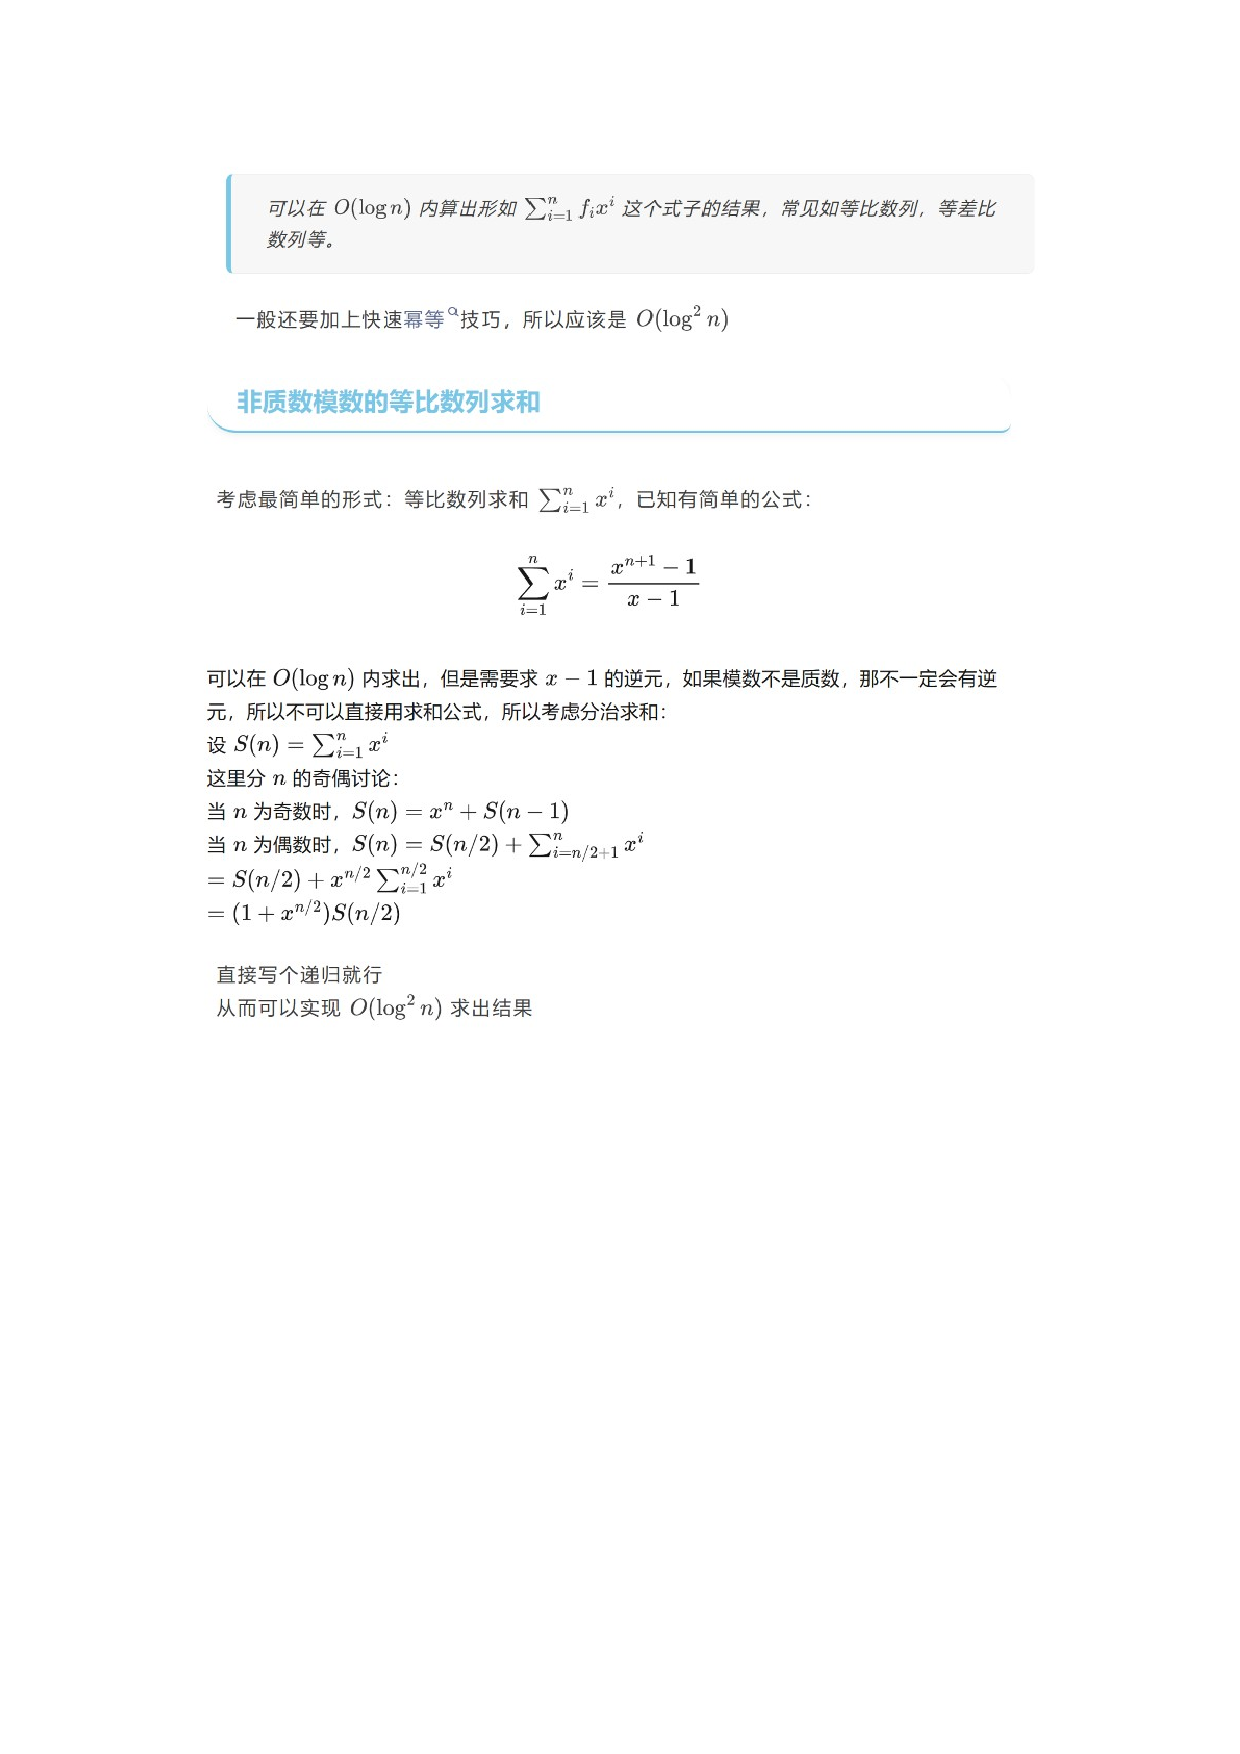
\includepdf[pages=-]{doc_tmp/math_fenzhi.pdf}

\subsection{莫比乌斯反演的套路}

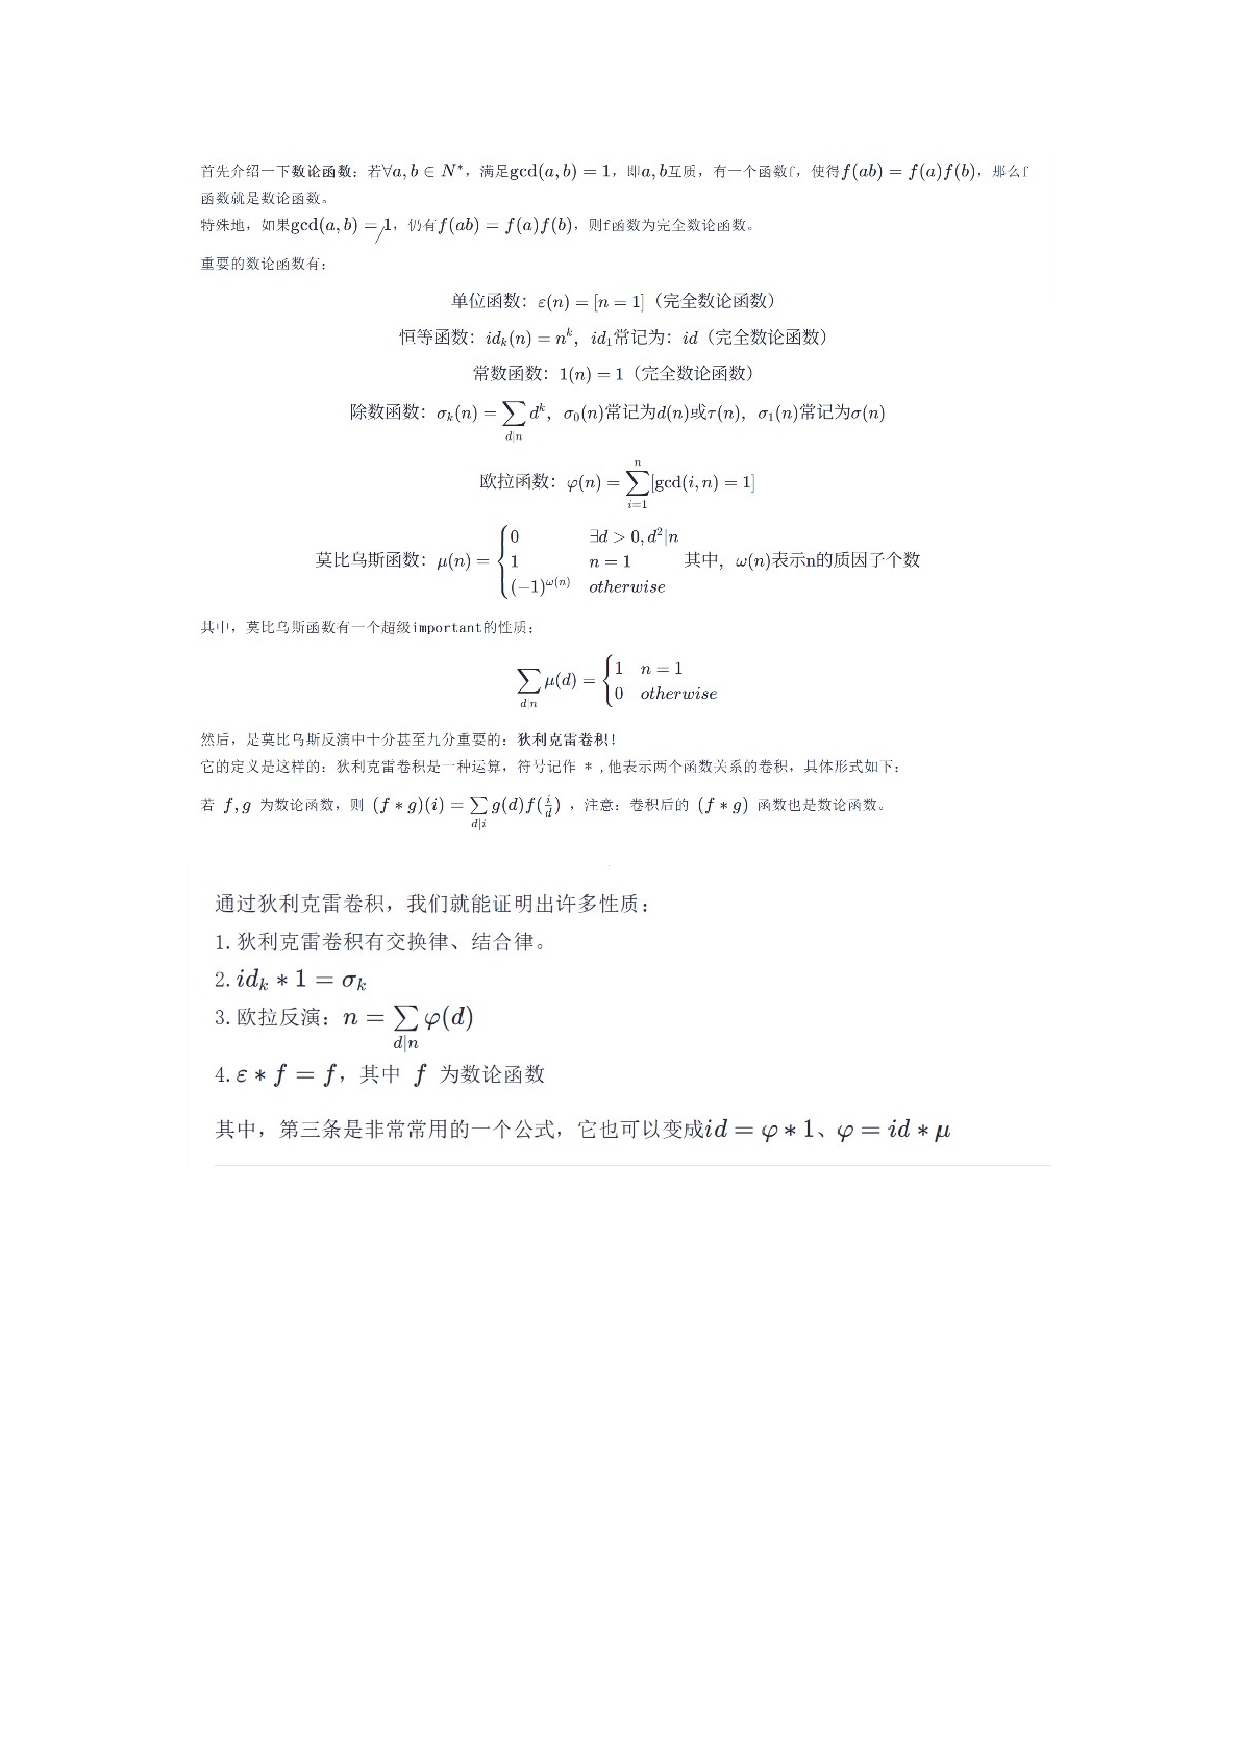
\includepdf[pages=-]{doc_tmp/math_mobius.pdf}

\subsection{exgcd}

\begin{lstlisting}
解方程：ax+by=gcd(a,b)


int exgcd(int a, int b, int &x, int &y)
{
    if(b==0){
        x=1; y=0;
        return a;
    }
    int g = exgcd(b, a%b, x, y); 
    int tmp = x;
    x = y, y = tmp - y*(a/b);
    return g;
}
\end{lstlisting}

\subsection{CRT}

\begin{lstlisting}
给 n 个同余方程组 x=a(mod b)，要解出最小的x

#include<bits/stdc++.h>
using namespace std;
typedef unsigned long long ull;
int n;
ull ans;
long long b[15],a[15];
ull A=1,Ai[15];
ull invA[15];

void exgcd(ull a,ull b,ull &x,ull &y)
{
	if(b==0){
		x=1;
		y=0;
		return ;
	}
	exgcd(b,a%b,x,y);
	ull gcd=x;
	x=y,y=gcd-y*(a/b);
}
int main()
{
	scanf("%d",&n);
	for(int i=1;i<=n;i++)
		scanf("%lld%lld",&a[i],&b[i]),A=(ull)A*a[i];
	for(int i=1;i<=n;i++)
		Ai[i]=A/a[i];
	// 整数解为：x= (b1*A1*invA1)*...*(bn*An*invAn) 
	// 此处的 invA 表示在 mod a[i] 意义下 Ai[i] 的逆元
	for(int i=1;i<=n;i++)
	{
		ull x=0,y=0;
		exgcd(Ai[i],a[i],x,y);
		invA[i]=(x+a[i])%a[i];
	}
	for(int i=1;i<=n;i++)
	{
		ans+=b[i]*invA[i]*Ai[i]%A;
		ans%=A;
	}
	cout<<ans%A;
	return 0;
}
\end{lstlisting}

\subsection{数论公式}

\begin{itemize}
  \item 欧拉定理：若 $\gcd(a,n)=1$，则
  \[a^{\varphi(n)}\equiv 1\pmod n.\]
  \item 扩展欧拉定理：对任意正整数 $b$，
  \[
  a^b\equiv
  \begin{cases}
    a^b, & b<\varphi(n),\\
    a^{b\bmod\varphi(n)+\varphi(n)}, & b\ge\varphi(n)
  \end{cases}
  \pmod n.
  \]
  \item 费马小定理：$p$ 为素数且 $p\not\mid a$ 时 $a^{p-1}\equiv 1\pmod p$；等价形式 $a^p\equiv a\pmod p$。
  \item 卢卡斯定理：$p$ 为素数时
  \[
  \binom{n}{m}\equiv\binom{n\bmod p}{m\bmod p}\cdot\binom{\lfloor n/p\rfloor}{\lfloor m/p\rfloor}\pmod p.
  \]
  \item 裴蜀定理：方程 $\sum_{i=1}^{k}a_ix_i=c$ 有整数解当且仅当 $\gcd(a_1,\dots,a_k)\mid c$；$k=2$ 时即 $ax+by=c$ 有解当且仅当 $\gcd(a,b)\mid c$。
  \item 二次剩余：$p$ 为奇素数、$a\not\equiv 0\pmod p$，则 $a$ 是模 $p$ 的二次剩余当且仅当
  \[a^{(p-1)/2}\equiv 1\pmod p\]
  （欧拉判别法）；$a^{(p-1)/2}\equiv -1$ 时为非二次剩余。Cipolla 算法可在 $O(\log p)$ 内求出 $\sqrt{a}\bmod p$。
  \item 狄利克雷卷积：$(f*g)(n)=\sum_{d\mid n}f(d)\,g\!\left(\frac{n}{d}\right)$。常见展开式
  \[\varepsilon=\mu*1,\qquad d=1*1,\qquad \sigma=\mathrm{id}*1,\qquad \varphi=\mu*\mathrm{id},\]
  其中 $\varepsilon(n)=[n=1]$、$\mathrm{id}(n)=n$。莫比乌斯反演：$f=g*1\iff g=f*\mu$。
  \item 约数个数与约数和：若 $n=\prod_{i=1}^{s}p_i^{e_i}$，则
  \[d(n)=\prod_{i=1}^{s}(e_i+1),\qquad \sigma(n)=\prod_{i=1}^{s}\frac{p_i^{e_i+1}-1}{p_i-1}.\]
  \item 原根与阶：$\mathrm{ord}_p(a)$ 为使 $a^k\equiv 1\pmod p$ 成立的最小正整数 $k$，必有 $\mathrm{ord}_p(a)\mid p-1$；$g$ 是模素数 $p$ 的原根当且仅当 $\mathrm{ord}_p(g)=p-1$。模 $n$ 原根存在的充要条件是 $n=2,4,p^k,2p^k$（$p$ 为奇素数）。求原根：分解 $p-1=\prod q_i^{c_i}$，枚举 $g$ 并验证 $g^{(p-1)/q_i}\not\equiv 1\pmod p$ 对所有素因子 $q_i$ 成立。
  \item BSGS（离散对数）：解 $a^x\equiv b\pmod p$，$\gcd(a,p)=1$。取 $M=\lceil\sqrt p\rceil$，令 $x=iM-j$，则 $a^{iM}\equiv b\,a^{j}\pmod p$；预处理右侧 $j\in[0,M)$ 的哈希表，枚举左侧 $i\in[0,M)$ 查表，复杂度 $O(\sqrt p)$，并特判 $b\equiv 1\pmod p$ 时 $x=0$。
\end{itemize}

\subsection{BSGS}

\begin{lstlisting}
BSGS解方程求x： b^x=n (mod p)

#include<bits/stdc++.h>
using namespace std;
typedef long long ll;
unordered_map<ll, ll> mp;
ll p,b,n,s;
int main() {
	cin>>p>>b>>n, s=sqrt(p)+1;
	for(ll y=1, pw=n*b%p; y<=s; y++, pw=pw*b%p) mp[pw%p]=y;
	
	ll t=1;
	for(ll i=1; i<=s; i++) t=t*b%p;
	for(ll x=1, pw=t; x<=s; x++, pw=pw*t%p)
		if(mp[pw])
			return cout<<x*s-mp[pw], 0;
    
	cout<<"no solution";
	return 0;
}
\end{lstlisting}

\subsection{Pollard Rho 素数判定}

\begin{lstlisting}
输入一个 N，判定其是否为素数（求其最大质因子）时间复杂度O(N^0.25)

#include <bits/stdc++.h>
using namespace std;

typedef long long ll;
typedef __int128 lll;

ll RandInt(ll l , ll r) {
	static mt19937 Rand(time(0));
	uniform_int_distribution<ll> dis(l, r);
	return dis(Rand);
}

ll Quick_Power(ll a , ll b , ll p) {
	ll res = 1;
	while(b) {
		if(b & 1) res = (lll)res * a % p;
		a = (lll)a * a % p;
		b >>= 1;
	}
	return res;
}

bool Miller_Rabin(ll n) {
	if(n < 3 || n % 2 == 0) return n == 2;
	ll a = n - 1 , b = 0;
	while(a % 2 == 0) {
		a /= 2;
		b++;
	}
	for(int i = 1 , j; i <= 10; i++) {
		ll x = RandInt(2 , n - 1);
		ll v = Quick_Power(x , a , n);
		if(v == 1) continue;
		for(j = 0; j < b; j++) {
			if(v == n - 1) break;
			v = (lll) v * v % n;
		}
		if(j == b) return 0;
	}
	return 1; 
}

ll F(ll x , ll c , ll n) {
	return ((lll)x * x + c) % n;
}

ll Pollard_Rho(ll n) {
	ll s = 0 , t = 0;
	ll c = RandInt(1 , n - 1);
	int step = 0 , goal = 1;
	ll value = 1;
	for(goal = 1;; goal <<= 1, s = t , value = 1) {
		for(step = 1; step <= goal; step++) {
			t = F(t , c , n);
			value = ((lll)value * abs(t - s)) % n;
			if(step % 127 == 0) {
				ll d = __gcd(value , n);
				if(d > 1) return d;
			}
		}
		ll d = __gcd(value , n);
		if(d > 1) return d;
	}
}

ll Ans;

void Fac(ll n) {
	if(n <= Ans || n < 2) return;
	if(Miller_Rabin(n)) {
		Ans = max(Ans , n);
		return;
	}
	ll p = n;
	while(p == n) p = Pollard_Rho(n);
	while((n % p) == 0) n /= p;
	Fac(n);
	Fac(p); 
}

ll T , N;

int main() {
	cin >> T;
	while(T--) {
		Ans = 0;
		cin >> N;
		Fac(N);
		if(Ans == N) {
			cout << "Prime" << endl;
		}
		else {
			cout << Ans << endl;
		}
	}
	return 0;
} 
\end{lstlisting}

\subsection{组合计数}

\begin{itemize}
  \item 容斥原理：
  \[\left|\bigcup_{i=1}^{n}A_i\right|=\sum_{\emptyset\ne S\subseteq[n]}(-1)^{|S|+1}\left|\bigcap_{i\in S}A_i\right|.\]
  补集形式：$\left|\bigcap_{i=1}^{n}\overline{A_i}\right|=\sum_{S\subseteq[n]}(-1)^{|S|}\left|\bigcap_{i\in S}A_i\right|$（$S=\emptyset$ 一项为全集大小）。min-max 容斥：$\max(S)=\sum_{\emptyset\ne T\subseteq S}(-1)^{|T|+1}\min(T)$，$\min(S)=\sum_{\emptyset\ne T\subseteq S}(-1)^{|T|+1}\max(T)$。
  \item 二项式系数恒等式：
  \[\binom{n}{k}=\binom{n}{n-k},\qquad \binom{n}{k}=\binom{n-1}{k}+\binom{n-1}{k-1},\]
  \[\sum_{k=0}^{n}\binom{n}{k}=2^n,\qquad \sum_{k=0}^{n}(-1)^k\binom{n}{k}=[n=0],\]
  \[\sum_{k=0}^{n}k\binom{n}{k}=n\,2^{n-1},\qquad k\binom{n}{k}=n\binom{n-1}{k-1}.\]
  上指标翻转：$\binom{-n}{k}=(-1)^k\binom{n+k-1}{k}$。
  \item 范德蒙德卷积：
  \[\sum_{k=0}^{r}\binom{n}{k}\binom{m}{r-k}=\binom{n+m}{r},\]
  推论 $\sum_{k}\binom{n}{k}^{2}=\binom{2n}{n}$。
  \item 卡特兰数：$C_n=\dfrac{1}{n+1}\binom{2n}{n}$，$C_0=C_1=1$，递推 $C_n=\sum_{i=0}^{n-1}C_iC_{n-1-i}$、$C_n=\dfrac{4n-2}{n+1}C_{n-1}$。组合意义：$n$ 对括号的合法匹配数、$n$ 个结点的二叉树形态数、$n\times n$ 网格不越过对角线的单调路径数、$n$ 个元素的出栈序列数。
  \item 第一类斯特林数 $\begin{bmatrix}n\\k\end{bmatrix}$：把 $n$ 个不同元素排成恰好 $k$ 个非空循环（轮换）的方案数，组合意义上即「$k$ 个环的置换」的个数，递推
  \[\begin{bmatrix}n\\k\end{bmatrix}=(n-1)\begin{bmatrix}n-1\\k\end{bmatrix}+\begin{bmatrix}n-1\\k-1\end{bmatrix},\]
  且 $\sum_{k}\begin{bmatrix}n\\k\end{bmatrix}x^{k}=x^{\overline n}=x(x+1)\cdots(x+n-1)$（上升幂）。
  \item 第二类斯特林数 $\begin{Bmatrix}n\\k\end{Bmatrix}$：把 $n$ 个不同元素划分为恰好 $k$ 个非空无序子集的方案数（无标号盒子），递推
  \[\begin{Bmatrix}n\\k\end{Bmatrix}=k\begin{Bmatrix}n-1\\k\end{Bmatrix}+\begin{Bmatrix}n-1\\k-1\end{Bmatrix},\]
  且 $x^{n}=\sum_{k}\begin{Bmatrix}n\\k\end{Bmatrix}x^{\underline k}$（下降幂）。
  \item 错排：$D_n=(n-1)(D_{n-1}+D_{n-2})$，$D_0=1$、$D_1=0$；通项
  \[D_n=n!\sum_{k=0}^{n}\frac{(-1)^k}{k!}.\]
  \item 贝尔数：$B_n$ 是 $n$ 元集合的划分方案数，$B_n=\sum_{k}\begin{Bmatrix}n\\k\end{Bmatrix}$，$B_0=1$；
  \[B_{n+1}=\sum_{k=0}^{n}\binom{n}{k}B_k,\qquad \sum_{n\ge0}\frac{B_n}{n!}x^{n}=e^{e^x-1}.\]
\end{itemize}

\subsection{生成函数与伯努利数}

\begin{itemize}
  \item 生成函数：普通型 $\mathrm{OGF}$ 为 $A(x)=\sum_{n\ge0}a_nx^{n}$，指数型 $\mathrm{EGF}$ 为 $\widehat A(x)=\sum_{n\ge0}a_n\dfrac{x^{n}}{n!}$。常用展开：
  \[\frac{1}{1-x}=\sum_{n\ge0}x^{n},\qquad e^{x}=\sum_{n\ge0}\frac{x^{n}}{n!},\qquad \ln\frac{1}{1-x}=\sum_{n\ge1}\frac{x^{n}}{n}.\]
  用途区别：$\mathrm{EGF}$ 适合带标号对象的拼接与划分，$\mathrm{OGF}$ 适合无标号计数。
  \item 伯努利数：由生成函数定义
  \[\frac{x}{e^{x}-1}=\sum_{n\ge0}\frac{B_n}{n!}x^{n},\]
  有 $B_0=1$、$B_1=-\dfrac{1}{2}$、$B_{2n+1}=0\ (n\ge1)$。用于求幂和：
  \[\sum_{k=0}^{m-1}k^{n}=\frac{1}{n+1}\sum_{j=0}^{n}\binom{n+1}{j}B_j\,m^{\,n+1-j}.\]
\end{itemize}

\subsection{拉格朗日插值}

\begin{lstlisting}
给n个点，确定一条曲线f，然后求f(k)

#include<bits/stdc++.h>
using namespace std;

long long n,k;
long long y[2007],x[2007];
const long long mod=998244353;
long long ans;
long long quickpow(long long a,long long b)
{
	long long res=1;
	while(b)
	{
		if(b&1)res=res*a%mod;
		a=a*a%mod;
		b>>=1;
	}
	return res;
}
long long inv(long long k)
{
	return quickpow(k,mod-2);
}

int main()
{
	cin>>n>>k;
	for(int i=1;i<=n;i++)
		cin>>x[i]>>y[i];
	for(int i=1;i<=n;i++)
	{
		long long s1=y[i]%mod;
		long long s2=1ll;
		for(int j=1;j<=n;j++)
		{
			if(i==j)continue;
			s1=s1*(k-x[j])%mod;
			s2=s2*((x[i]-x[j])%mod)%mod;
		}
		ans+=s1*inv(s2)%mod;
		ans=(ans+mod)%mod;
	}
	cout<<ans;
	return 0;
}
\end{lstlisting}

\section{数据结构}

\subsection{LCT动态双连通分量}

\begin{lstlisting}
#include <bits/stdc++.h>
using namespace std;
struct Splay{
	int ch[3],fa,val,sm,rev,cov;
}a[1000010];
struct Edg{
	int u,v,ext;
}edg[1000010];
struct Qus{
	int opt,u,v,id;
}q[1000010];
int n,m,cnt,ans[1000010],cntans;
bool isroot(int x){
	if(a[a[x].fa].ch[0]==x||a[a[x].fa].ch[1]==x){
		return 0;
	}
	return 1;
}
void pushdown(int p){
	if(a[p].cov){
		if(a[p].ch[0]){
			a[a[p].ch[0]].val=0;
			a[a[p].ch[0]].sm=0;
			a[a[p].ch[0]].cov=1;
		}
		if(a[p].ch[1]){
			a[a[p].ch[1]].val=0;
			a[a[p].ch[1]].sm=0;
			a[a[p].ch[1]].cov=1;
		}
		a[p].cov=0;
	}
	if(a[p].rev){
		swap(a[p].ch[0],a[p].ch[1]);
		a[a[p].ch[0]].rev^=1;
		a[a[p].ch[1]].rev^=1;
		a[p].rev=0;
	}
	return ;
}
void pushup(int p){
	a[p].sm=a[p].val+a[a[p].ch[0]].sm+a[a[p].ch[1]].sm;
}
void push(int p){
	if(!isroot(p)){
		push(a[p].fa);
	}
	pushdown(p);
}
void rotate(int x){
	int y=a[x].fa;
	int z=a[y].fa;
	int kid=a[y].ch[1]==x;
	if(!isroot(y)){
		a[z].ch[a[z].ch[1]==y]=x;
	}
	a[x].fa=z;
	a[y].ch[kid]=a[x].ch[kid^1];
	a[a[x].ch[kid^1]].fa=y;
	a[x].ch[kid^1]=y;
	a[y].fa=x;
	pushup(y);
	pushup(x);
	return ;
}
void splay(int x){
	push(x);
	while(!isroot(x)){
		int y=a[x].fa;
		int z=a[y].fa;
		if(!isroot(y)){
			(a[z].ch[1]==y)^(a[y].ch[1]==x)?rotate(x):rotate(y);
		}
		rotate(x);
	}
	return ;
}
void access(int x){
	int y=0;
	while(x){
		splay(x);
		a[x].ch[1]=y;
		pushup(x);
		y=x,x=a[x].fa;
	}
	return ;
}
void makeroot(int x){
	access(x);
	splay(x);
	a[x].rev^=1;
	return ;
}
void split(int x,int y){
	makeroot(x);
	access(y);
	splay(y);
	return ;
}
int ask(int x,int y){
	split(x,y);
	return a[y].sm;
}
int findroot(int x){
	access(x);
	splay(x);
	while(a[x].ch[0]){
		pushdown(x);
		x=a[x].ch[0];
	}
	splay(x);
	return x;
}
void link(int x,int y){
	makeroot(x);
	if(findroot(y)==x){
		return ;
	}
	a[x].fa=y;
	return ;
}
void cut(int x,int y){
	makeroot(x);
	if(findroot(y)==x&&a[y].fa==x&&(!a[y].ch[0])){
		a[y].fa=0;
		pushup(x);
	}
	return ;
}
void add(int x,int y,int eid){
	if(findroot(x)==findroot(y)){
        split(x,y);
        a[y].cov=1;
        pushdown(y);
    }
    else{
        a[eid].val=1;
        a[eid].sm=1;
        link(x,eid);
        link(eid,y);
    }
}
signed main(){
	cin>>n>>m;
	for(int i=1;i<=m;i++){
		cin>>edg[i].u>>edg[i].v;
		if(edg[i].u>edg[i].v){
			swap(edg[i].u,edg[i].v);
		}
		edg[i].ext=1;
	}
	while(1){
		int opt;
		cin>>opt;
		if(opt==-1){
			break;
		}
		cnt++;
		q[cnt].opt=opt;
		cin>>q[cnt].u>>q[cnt].v;
		if(opt==0){
			if(q[cnt].u>q[cnt].v){
				swap(q[cnt].u,q[cnt].v);
			}
			for(int j=1;j<=m;j++){
				if(edg[j].u==q[cnt].u&&edg[j].v==q[cnt].v){
					q[cnt].id=j;
					edg[j].ext=0;
					break;
				}
			}
		}
	}
	for(int i=1;i<=m;i++){
		if(edg[i].ext){
			int u=edg[i].u,v=edg[i].v;
			int eid=n+i;
			if(findroot(u)!=findroot(v)){
				a[eid].val=1;
				a[eid].sm=1;
				link(u,eid);
				link(eid,v);
			}
			else{
				split(u,v);
				a[v].cov=1;
				pushdown(v);
				a[eid].val=0;
				a[eid].sm=0;
				link(u,eid);
				link(eid,v);
			}
		}
	}
	for(int i=cnt;i>=1;i--){
		if(q[i].opt==0){
			int eid=n+q[i].id;
			add(q[i].u,q[i].v,eid);
		}
		else{
			ans[++cntans]=ask(q[i].u,q[i].v);
		}
	}
	for(int i=cntans;i>=1;i--){
		cout<<ans[i]<<endl;
	}
}
/*
A,B 两星球之间，如果某条航线不存在，
就无法从 A 星球抵达 B 星球，我们则称这条航线为关键航线。
若 op=1，则后接两个整数 u,v，表示询问当前 u,v 两星球之间有多少关键航线。
若 op=0，则后接两个整数 u,v，表示 u,v 之间的航线被破坏。
若 op=-1，则表示输入结束，后面不再存在操作。

逆序完成操作，因为只有加边操作，
所以实际上只有关键边变非关键边，而不存在非关键边变成关键边。
一条关键边对于任意两个过其的点都是关键边
对每个边维护一下其是否为关键边，如果是其边权为1，否则其边权为0 

在 LCT 中，通常节点代表树上的点。为了维护边的信息（比如这条边是不是桥），
代码采用了经典的技巧：每一条无向边 (u,v) 视为一个新的虚拟节点。
假设原图有n个点，第i条边对应的虚拟节点编号为n+i
在 LCT 中，原本连接 u和 v的边，变成了两条树边：u(n+i)和 v(n+i)。
边的属性（是否为关键航线）存储在这个虚拟节点 (n+i)的val字段中：
val = 1：表示该边是关键航线（桥）。
val = 0：表示该边不是关键航线（在某个环中）。

LCT 限制：只能维护点上的信息。
解决方案：把每一条边 (u,v) 变成一个新节点（即虚拟节点 eid = n + i），
然后把原来的边拆成两条边： u→eid和 eid→v 。

*/
\end{lstlisting}

\subsection{LCT动态树}

\begin{lstlisting}
#include <bits/stdc++.h>
using namespace std;
struct Splay{
	int ch[3],fa,val,sm,rev;
}a[1000010];
int n,m;
bool isroot(int x){
	if(a[a[x].fa].ch[0]==x||a[a[x].fa].ch[1]==x){
		return 0;
	}
	return 1;
}
void pushdown(int p){
	if(a[p].rev){
		swap(a[p].ch[0],a[p].ch[1]);
		a[a[p].ch[0]].rev^=1;
		a[a[p].ch[1]].rev^=1;
		a[p].rev=0;
	}
	return ;
}
void pushup(int p){
	a[p].sm=a[p].val^a[a[p].ch[0]].sm^a[a[p].ch[1]].sm;
}
void push(int p){
	if(!isroot(p)){
		push(a[p].fa);
	}
	pushdown(p);
}
void rotate(int x){
	int y=a[x].fa;
	int z=a[y].fa;
	int kid=a[y].ch[1]==x;
	if(!isroot(y)){
		a[z].ch[a[z].ch[1]==y]=x;
	}
	a[x].fa=z;
	a[y].ch[kid]=a[x].ch[kid^1];
	a[a[x].ch[kid^1]].fa=y;
	a[x].ch[kid^1]=y;
	a[y].fa=x;
	pushup(y);
	pushup(x);
	return ;
}
void splay(int x){
	push(x);
	while(!isroot(x)){
		int y=a[x].fa;
		int z=a[y].fa;
		if(!isroot(y)){
			(a[z].ch[1]==y)^(a[y].ch[1]==x)?rotate(x):rotate(y);
		}
		rotate(x);
	}
	return ;
}
void access(int x){
	int y=0;
	while(x){
		splay(x);
		a[x].ch[1]=y;
		pushup(x);
		y=x,x=a[x].fa;
	}
	return ;
}
void makeroot(int x){
	access(x);
	splay(x);
	a[x].rev^=1;
	return ;
}
void split(int x,int y){
	makeroot(x);
	access(y);
	splay(y);
	return ;
}
int ask(int x,int y){
	split(x,y);
	return a[y].sm;
}
int findroot(int x){
	access(x);
	splay(x);
	while(a[x].ch[0]){
		pushdown(x);
		x=a[x].ch[0];
	}
	splay(x);
	return x;
}
void link(int x,int y){
	makeroot(x);
	if(findroot(y)==x){
		return ;
	}
	a[x].fa=y;
	return ;
}
void cut(int x,int y){
	makeroot(x);
	if(findroot(y)==x&&a[y].fa==x&&(!a[y].ch[0])){
		a[y].fa=0;
		pushup(x);
	}
	return ;
}
void change(int x,int y){
	splay(x);
	a[x].val=y;
	pushup(x);
	return ;
}
signed main(){
	cin>>n>>m;
	for(int i=1;i<=n;i++){
		cin>>a[i].val;
	}
	for(int i=1;i<=m;i++){
		int opt,x,y;
		cin>>opt>>x>>y;
		if(opt==0){
			cout<<ask(x,y)<<endl;
		}
		if(opt==1){
			link(x,y);
		}
		if(opt==2){
			cut(x,y);
		}
		if(opt==3){
			change(x,y);
		}
	}
}
/*
给定 n 个点以及每个点的权值，要你处理接下来的 m 个操作。
操作有四种，操作从 0 到 3 编号。点从 1 到 n 编号。
 
0 x y 代表询问从 x 到 y 的路径上的点的权值的 xor 和。保证 x 到 y 是联通的。
1 x y 代表连接 x 到 y，若 x 到 y 已经联通则无需连接。
2 x y 代表删除边 (x,y)，不保证边 (x,y) 存在。
3 x y 代表将点 x 上的权值变成 y。

*/
\end{lstlisting}

\subsection{LCT动态生成树}

\begin{lstlisting}
#include <bits/stdc++.h>
#define int long long
using namespace std;
int n,m,q,id,fa[1000010],del[1000010];
map<pair<int,int>,int> edg;
struct Edge{
    int u,v,w,id;
}edgg[1000010],temp[1000010];
struct Query{
    int k,u,v,ans;
}qs[1000010];
bool cmp(Edge a,Edge b){
    return a.w<b.w;
}
int Find(int x){
	if(fa[x]==x){
		return x;
	}
	return fa[x]=Find(fa[x]);
}
struct Splay{
    int fa,ch[3],rev,mx,val;
}a[1000010];
bool isroot(int x){
    if(a[a[x].fa].ch[0]==x||a[a[x].fa].ch[1]==x){
        return 0;
    }
    return 1;
}
void pushup(int x){
	a[x].mx=x;
    if(a[x].ch[0]&&a[a[a[x].ch[0]].mx].val>a[a[x].mx].val){
        a[x].mx=a[a[x].ch[0]].mx;
    }
    if(a[x].ch[1]&&a[a[a[x].ch[1]].mx].val>a[a[x].mx].val){
        a[x].mx=a[a[x].ch[1]].mx;
    }
}
void pushdown(int x){
    if(a[x].rev){
        swap(a[x].ch[0],a[x].ch[1]);
        if(a[x].ch[0]){
        	a[a[x].ch[0]].rev^=1;
		}
        if(a[x].ch[1]){
        	a[a[x].ch[1]].rev^=1;
		}
        a[x].rev=0;
    }
    return ;
}
void push(int x){
    if(!isroot(x)){
        push(a[x].fa);
    }
    pushdown(x);
}
void rotate(int x){
    int y=a[x].fa;
    int z=a[y].fa;
    int kid=a[y].ch[1]==x;
    if(!isroot(y)){
        a[z].ch[a[z].ch[1]==y]=x;
    }
    a[x].fa=z;
    a[y].ch[kid]=a[x].ch[kid^1];
    a[a[x].ch[kid^1]].fa=y;
    a[x].ch[kid^1]=y;
    a[y].fa=x;
    pushup(y);
    pushup(x);
    return ;
}
void splay(int x){
    push(x);
    while(!isroot(x)){
        int y=a[x].fa;
        int z=a[y].fa;
        if(!isroot(y)) {
            (a[z].ch[1]==y)^(a[y].ch[1]==x)?rotate(x):rotate(y);
        }
        rotate(x);
    }
    return ;
}
void access(int x){
    int y=0;
    while(x){
        splay(x);
        a[x].ch[1]=y;
        pushup(x);
        y=x,x=a[x].fa;
    }
    return ;
}
void makeroot(int x){
    access(x);
    splay(x);
    a[x].rev^=1;
    return ;
}
void split(int x,int y){
    makeroot(x);
    access(y);
    splay(y);
    return ;
}
int findroot(int x){
    access(x);
    splay(x);
    pushdown(x); 
    while(a[x].ch[0]){
        pushdown(x);
        x=a[x].ch[0];
    }
    splay(x);
    return x;
}
void link(int x,int y){
    makeroot(x);
    if(findroot(y)!=x){
        a[x].fa=y;
    }
    return ;
}
void cut(int x,int y){
    makeroot(x);
    if(findroot(y)==x&&a[y].fa==x&&(!a[y].ch[0])){
    	a[x].ch[1]=0;
        a[y].fa=0;
        pushup(x);
    }
    return ;
}
int Que(int x,int y){
    split(x,y);
    return a[y].mx;
}
signed main(){
    cin>>n>>m>>q;
    for(int i=1;i<=n;i++){
        a[i].val=0;
        a[i].mx=i;
        fa[i]=i;
    }
    for(int i=1;i<=m;i++){
        int u,v,t;
        cin>>u>>v>>t;
        if(u>v){
        	swap(u,v);
		}
        edgg[i].u=u;
        edgg[i].v=v;
        edgg[i].w=t;
        edgg[i].id=i;
        edg[{u,v}]=i;
        a[n+i].val=t;
        a[n+i].mx=n+i;
    }
    for(int i=1;i<=q;i++){
        cin>>qs[i].k>>qs[i].u>>qs[i].v;
        if(qs[i].u>qs[i].v){
        	swap(qs[i].u,qs[i].v);
		}
        if(qs[i].k==2){
            int eid=edg[{qs[i].u,qs[i].v}];
            del[eid]=1;
        }
    }
    int cnt=0;
    for(int i=1;i<=m;i++){
        if(!del[i]){
            temp[++cnt]=edgg[i];
        }
    }
    sort(temp+1,temp+cnt+1,cmp);
    for(int i=1;i<=cnt;i++){
        int fu=Find(temp[i].u);
        int fv=Find(temp[i].v);
        if(fu!=fv) {
            fa[fu]=fv;
            link(temp[i].u,n+temp[i].id);
            link(temp[i].v,n+temp[i].id);
        }
    }
    for(int i=q;i>=1;i--){
        if(qs[i].k==1){
            split(qs[i].u,qs[i].v);
            qs[i].ans=a[a[qs[i].v].mx].val;
        }
		else{
            int eid=edg[{qs[i].u,qs[i].v}];
            int u=qs[i].u,v=qs[i].v,w=edgg[eid].w;
            split(u,v);
            int mx_n=a[v].mx;
            if(a[mx_n].val>w){
                int id=mx_n-n;
                cut(edgg[id].u,mx_n);
                cut(edgg[id].v,mx_n);
                link(u,n+eid);
                link(v,n+eid);
            }
        }
    }
    for(int i=1;i<=q;i++){
        if(qs[i].k==1){
            cout<<qs[i].ans<<endl;
        }
    }
    return 0;
}
/*
给一个n个点m条边的图，支持以下操作：
1 询问x到y所有路径中，路径上最大边权的最小值
2 删去一条边
*/
\end{lstlisting}

\subsection{LCT多标记}

\begin{lstlisting}
#include <bits/stdc++.h>
#define int long long
using namespace std;
const int md=51061;
struct Splay{
	int ch[3],fa,val,sm,rev,add,tim,siz;
}a[1000010];
int n,m;
bool isroot(int x){
	if(a[a[x].fa].ch[0]==x||a[a[x].fa].ch[1]==x){
		return 0;
	}
	return 1;
}
void pushdown(int p){
    if(!p){
    	return;	
	}
    if(a[p].rev){
        swap(a[p].ch[0],a[p].ch[1]);
        if(a[p].ch[0]){
        	a[a[p].ch[0]].rev^=1;
		}
        if(a[p].ch[1]){
        	a[a[p].ch[1]].rev^=1;
		}
        a[p].rev=0;
    }
    if(a[p].tim!=1){
        int t=a[p].tim;
        if(a[p].ch[0]){
            a[a[p].ch[0]].val=(a[a[p].ch[0]].val*t)%md;
            a[a[p].ch[0]].sm=(a[a[p].ch[0]].sm*t)%md;
            a[a[p].ch[0]].add=(a[a[p].ch[0]].add*t)%md;
            a[a[p].ch[0]].tim=(a[a[p].ch[0]].tim*t)%md;
        }
        if(a[p].ch[1]){
            a[a[p].ch[1]].val=(a[a[p].ch[1]].val*t)%md;
            a[a[p].ch[1]].sm=(a[a[p].ch[1]].sm*t)%md;
            a[a[p].ch[1]].add=(a[a[p].ch[1]].add*t)%md;
            a[a[p].ch[1]].tim=(a[a[p].ch[1]].tim*t)%md;
        }
        a[p].tim=1;
    }
    if(a[p].add){
        if(a[p].ch[0]){
            a[a[p].ch[0]].val=(a[a[p].ch[0]].val+a[p].add)%md;
            a[a[p].ch[0]].sm=(a[a[p].ch[0]].sm+a[p].add*a[a[p].ch[0]].siz)%md;
            a[a[p].ch[0]].add=(a[a[p].ch[0]].add+a[p].add)%md;
        }
        if(a[p].ch[1]){
            a[a[p].ch[1]].val=(a[a[p].ch[1]].val+a[p].add)%md;
            a[a[p].ch[1]].sm=(a[a[p].ch[1]].sm+a[p].add*a[a[p].ch[1]].siz)%md;
            a[a[p].ch[1]].add=(a[a[p].ch[1]].add+a[p].add)%md;
        }
        a[p].add=0;
    }
}
void pushup(int p){
	if(!p){
		return ;
	}
	a[p].siz=1+a[a[p].ch[0]].siz+a[a[p].ch[1]].siz;
	a[p].sm=a[p].val+a[a[p].ch[0]].sm+a[a[p].ch[1]].sm;
	a[p].sm%=md;
	return ;
}
void push(int p){
	if(!isroot(p)){
		push(a[p].fa);
	}
	pushdown(p);
}
void rotate(int x){
	int y=a[x].fa;
	int z=a[y].fa;
	int kid=a[y].ch[1]==x;
	if(!isroot(y)){
		a[z].ch[a[z].ch[1]==y]=x;
	}
	a[x].fa=z;
	a[y].ch[kid]=a[x].ch[kid^1];
	a[a[x].ch[kid^1]].fa=y;
	a[x].ch[kid^1]=y;
	a[y].fa=x;
	pushup(y);
	pushup(x);
	return ;
}
void splay(int x){
	push(x);
	while(!isroot(x)){
		int y=a[x].fa;
		int z=a[y].fa;
		if(!isroot(y)){
			(a[z].ch[1]==y)^(a[y].ch[1]==x)?rotate(x):rotate(y);
		}
		rotate(x);
	}
	return ;
}
void access(int x){
	int y=0;
	while(x){
		splay(x);
		a[x].ch[1]=y;
		pushup(x);
		y=x,x=a[x].fa;
	}
	return ;
}
void makeroot(int x){
	access(x);
	splay(x);
	a[x].rev^=1;
	return ;
}
void split(int x,int y){
	makeroot(x);
	access(y);
	splay(y);
	return ;
}
int ask(int x,int y){
	split(x,y);
	return a[y].sm;
}
int findroot(int x){
	access(x);
	splay(x);
	while(a[x].ch[0]){
		pushdown(x);
		x=a[x].ch[0];
	}
	splay(x);
	return x;
}
void link(int x,int y){
	makeroot(x);
	if(findroot(y)==x){
		return ;
	}
	a[x].fa=y;
	return ;
}
void cut(int x,int y){
	makeroot(x);
	if(findroot(y)==x&&a[y].fa==x&&(!a[y].ch[0])){
		a[y].fa=0;
		pushup(x);
	}
	return ;
}
void change(int x,int y){
	splay(x);
	a[x].val=y;
	pushup(x);
	return ;
}
void add(int x,int y,int v){
	split(x,y);
	a[y].add+=v;
	a[y].val+=v;
	a[y].sm+=v*a[y].siz;
	a[y].sm%=md;
	return ;
}
void tim(int x,int y,int v){
	split(x,y);
	a[y].add*=v;
	a[y].val*=v;
	a[y].tim*=v;
	a[y].sm*=v;
	a[y].sm%=md;
	return ;
}
signed main(){
	cin>>n>>m;
	for(int i=1;i<=n;i++){
		a[i].sm=a[i].val=a[i].tim=a[i].siz=1;
	}
	for(int i=1;i<n;i++){
		int a,b;
		cin>>a>>b;
		link(a,b);
	}
	for(int i=1;i<=m;i++){
		int a,b,c,d;
		char opt;
		cin>>opt;
		if(opt=='+'){
			cin>>a>>b>>c;
			add(a,b,c);
		}
		if(opt=='-'){
			cin>>a>>b>>c>>d;
			cut(a,b);
			link(c,d);
		}
		if(opt=='*'){
			cin>>a>>b>>c;
			tim(a,b,c);
		}
		if(opt=='/'){
			cin>>a>>b;
			cout<<ask(a,b)<<endl;
		}
	}
}
/*
+ u v c:将u到v路径上的点权加上c
- u1 v1 u2 v2：将树中原有的边 (u1,v1) 删除，加入一条新边 (u2,v 2)，
保证操作完之后仍然是一棵树；
* u v c：将 u 到 v 的路径上的点的权值都乘上自然数 c；
/ u v：询问 u 到 v 的路径上的点的权值和，将答案对 51061 取模。

*/
\end{lstlisting}

\subsection{LCT维护子树大小}

\begin{lstlisting}
#include <bits/stdc++.h>
#define int long long
using namespace std;
int n,m;
struct Splay{
    int fa,ch[3],siz,si,rev;
} a[1000010];
bool isroot(int x){
    if(a[a[x].fa].ch[0]==x||a[a[x].fa].ch[1]==x){
        return 0;
    }
    return 1;
}
void pushup(int x) {
    a[x].siz=a[a[x].ch[0]].siz+a[a[x].ch[1]].siz+1+a[x].si;
}
void pushdown(int x){
    if(a[x].rev){
        swap(a[x].ch[0],a[x].ch[1]);
        if(a[x].ch[0]){
        	a[a[x].ch[0]].rev^=1;
		}
        if(a[x].ch[1]){
        	a[a[x].ch[1]].rev^=1;
		}
        a[x].rev=0;
    }
    return ;
}
void push(int x){
    if(!isroot(x)){
        push(a[x].fa);
    }
    pushdown(x);
}
void rotate(int x){
    int y=a[x].fa;
    int z=a[y].fa;
    int kid=a[y].ch[1]==x;
    if(!isroot(y)){
        a[z].ch[a[z].ch[1]==y]=x;
    }
    a[x].fa=z;
    a[y].ch[kid]=a[x].ch[kid^1];
    a[a[x].ch[kid^1]].fa=y;
    a[x].ch[kid^1]=y;
    a[y].fa=x;
    pushup(y);
    pushup(x);
    return ;
}
void splay(int x){
    push(x);
    while(!isroot(x)){
        int y=a[x].fa;
        int z=a[y].fa;
        if(!isroot(y)) {
            (a[z].ch[1]==y)^(a[y].ch[1]==x)?rotate(x):rotate(y);
        }
        rotate(x);
    }
    return ;
}
void access(int x){
    int y=0;
    while(x){
        splay(x);
		a[x].si+=a[a[x].ch[1]].siz;
        a[x].ch[1]=y;
        a[x].si-=a[y].siz;
        pushup(x);
        y=x,x=a[x].fa;
    }
    return ;
}
void makeroot(int x){
    access(x);
    splay(x);
    a[x].rev^=1;
    return ;
}
void split(int x,int y){
    makeroot(x);
    access(y);
    splay(y);
    return ;
}
int findroot(int x){
    access(x);
    splay(x);
    pushdown(x); 
    while(a[x].ch[0]){
        pushdown(x);
        x=a[x].ch[0];
    }
    splay(x);
    return x;
}
void link(int x,int y){
    makeroot(x);
    makeroot(y);
    a[x].fa=y;
    a[y].si+=a[x].siz;
    pushup(y);
    return ;
}
void cut(int x,int y){
    makeroot(x);
    if(findroot(y)==x&&a[y].fa==x&&(!a[y].ch[0])){
    	a[x].ch[1]=0;
        a[y].fa=0;
        pushup(x);
        return ;
    }
    return ;
}
void Qus(int x,int y){
	split(x,y);
    cut(x,y);
    makeroot(x);
    makeroot(y);
    pushup(x);
    pushup(y);
    cout<<a[x].siz*a[y].siz<<endl;
    link(x,y);
    return ;
}
signed main(){
    cin>>n>>m;
    for(int i=1;i<=n;i++){
        a[i].siz=1;
    }
    for(int i=1;i<=m;i++){
        char opt;
		int x,y;
        cin>>opt>>x>>y;
        if(opt=='A'){
            link(x,y);
        }
        if(opt=='Q'){
            Qus(x,y);
        }
    }
}
\end{lstlisting}

\subsection{ST表}

\begin{lstlisting}
#include <bits/stdc++.h>
#define int long long
using namespace std;
int n,m,a[1000010],st[100010][30],pw[100010];
int ask(int l,int r){
	int k=log(r-l+1)/log(2);
	return max(st[l][k],st[r-pw[k]+1][k]);
}
signed main(){
    cin>>n>>m;
    for(int i=1;i<=n;i++){
    	cin>>a[i];
    	st[i][0]=a[i];
	}
	int t=log(n)/log(2)+1;
	pw[0]=1;
	for(int i=1;i<=t;i++){
		pw[i]=pw[i-1]*2;
	}
	for(int k=1;k<=t;k++){
		for(int i=1;i+pw[k]-1<=n;i++){
			st[i][k]=max(st[i][k-1],st[i+pw[k-1]][k-1]);
		}
	}
	for(int i=1;i<=m;i++){
		int l,r;
		cin>>l>>r;
		cout<<ask(l,r)<<"\n";
	}
	return 0;
}
\end{lstlisting}

\subsection{Splay普通平衡树}

\begin{lstlisting}
#include <bits/stdc++.h>
using namespace std;
const int inf=1e9;
int n,root,tot;
struct splay{
	int ch[3],val,cnt;
	int size,fa;
}a[1000010];
void Update(int p){
	a[p].size=a[a[p].ch[0]].size+a[a[p].ch[1]].size+a[p].cnt;
}
void Rotate(int x){
	int y=a[x].fa;
	int z=a[y].fa;
	int kid=a[y].ch[1]==x;
	a[z].ch[a[z].ch[1]==y]=x;
	a[x].fa=z;
	a[y].ch[kid]=a[x].ch[kid^1];
	a[a[x].ch[kid^1]].fa=y;
	a[x].ch[kid^1]=y;
	a[y].fa=x;
	Update(y);
	Update(x);
}
void Splay(int x,int goal){
	while(a[x].fa!=goal){
		int y=a[x].fa;
		int z=a[y].fa;
		if(z!=goal){
			(a[z].ch[1]==y)^(a[y].ch[1]==x)?Rotate(x):Rotate(y);
		}
		Rotate(x);
	}
	if(goal==0){
		root=x;
	}
}
void Insert(int val){
	int now=root,fa=0;
	while(now&&a[now].val!=val){
		fa=now;
		now=a[now].ch[a[now].val<val];
	}
	if(now){
		a[now].cnt++;
	}
	else{
		now=++tot;
		if(fa){
			a[fa].ch[a[fa].val<val]=now;
			a[now].fa=fa;
		}
		a[now].val=val;
		a[now].size=a[now].cnt=1;
	}
	Splay(now,0);
}
void Search(int val){
	int now=root;
	if(!now){
		return ;
	}
	while(a[now].val!=val&&a[now].ch[a[now].val<val]){
		now=a[now].ch[a[now].val<val];
	}
	Splay(now,0);
}
int GetValByRank(int p,int rank){
	if(!p){
		return 0;
	}
	if(a[a[p].ch[0]].size>=rank){
		return GetValByRank(a[p].ch[0],rank);
	}
	if(a[a[p].ch[0]].size+a[p].cnt>=rank){
		return a[p].val;
	}
	return GetValByRank(a[p].ch[1],rank-a[a[p].ch[0]].size-a[p].cnt);
	
}
int GetPre(int val){
	Search(val);
	int pos=a[root].ch[0];
	while(a[pos].ch[1]){
		pos=a[pos].ch[1];
	}
	return pos;
}
int GetNext(int val){
	Search(val);
	int pos=a[root].ch[1];
	while(a[pos].ch[0]){
		pos=a[pos].ch[0];
	}
	return pos;
}
void Remove(int x){
	int pre_x=GetPre(x);
	int nxt_x=GetNext(x);
	Splay(pre_x,0);
	Splay(nxt_x,pre_x);
	int pos=a[root].ch[1];
	if(a[a[pos].ch[0]].cnt>1){
		a[a[pos].ch[0]].cnt--;
		Update(nxt_x);
		Update(pre_x);
		Splay(a[pos].ch[0],0);
		return ;
	}
	a[pos].ch[0]=0;
	Update(nxt_x);
	Update(pre_x);
	return ;
}
signed main(){
	cin>>n;
	Insert(-inf);
	Insert(inf);
	for(int i=1;i<=n;i++){
		int opt,x;
		cin>>opt>>x;
		if(opt==1){
			Insert(x);
		}
		if(opt==2){
			Remove(x);
		}
		if(opt==3){
			Insert(x);
			Search(x);
			cout<<a[a[root].ch[0]].size<<endl;
			Remove(x);
		}
		if(opt==4){
			cout<<GetValByRank(root,x+1)<<endl;
		}
		if(opt==5){
			Insert(x);
			cout<<a[GetPre(x)].val<<endl;
			Remove(x);
		}
		if(opt==6){
			Insert(x);
			cout<<a[GetNext(x)].val<<endl;
			Remove(x);
		}
	}
}
/*
您需要动态地维护一个可重集合 M，并且提供以下操作：

向 M 中插入一个数 x。
从 M 中删除一个数 x（若有多个相同的数，应只删除一个）。
查询 M 中有多少个数比 x 小，并且将得到的答案加一。
查询如果将 M 从小到大排列后，排名位于第 x 位的数。
查询 M 中 x 的前驱（前驱定义为小于 x，且最大的数）。
查询 M 中 x 的后继（后继定义为大于 x，且最小的数）。
对于操作 3,5,6，不保证当前可重集中存在数 x。

对于操作 5,6，保证答案一定存在。

输入格式
第一行为 n，表示操作的个数，下面 n 行每行有两个数 opt 和 x，opt 表示操作的序号（1≤opt≤6）。

输出格式
对于操作 3,4,5,6 每行输出一个数，表示对应答案。
*/
\end{lstlisting}

\subsection{Treap普通平衡树}

\begin{lstlisting}
维护多重集合：插入、删除一个数、查询x的排名、查询排名为x的数、查询x的前驱和后继

#include<bits/stdc++.h>
using namespace std;
#define INF (1<<30)

int n;
int opt,x;
const int N=1e5+10;

struct Treap{
	int l[N],r[N],val[N],rnd[N],size[N],w[N];
	// l[i],r[i] -> i的左右孩子
	// val[i] -> i的值
	// rnd[i] -> 分配的随机优先级 
	// w[i] -> i出现的次数
	// size[i] -> i为根的子树大小 
	int sz,ans,rt;
	// sz -> 给编号 
	// rt -> root
	// ans -> 答案（主要用于找前驱/后继） 
	 
	void pushup(int x) // 获取子树大小 
	{
		size[x]=size[l[x]]+size[r[x]]+w[x];
	}
	void Zip(int &k) // 左旋 k 节点  左旋就是让右孩子来做父亲 
	{
		int t=r[k]; // t 是左孩子
		r[k]=l[t];
		l[t]=k;
		size[t]=size[k];
		pushup(k);
		k=t;
	}
	void Zap(int &k) // 右旋 k 节点 
	{
		int t=l[k];
		l[k]=r[t];
		r[t]=k;
		size[t]=size[k];
		pushup(k);
		k=t;
	}
	void insert(int &k,int x) // 插入 x 
	{
		if(!k)
		{
			sz++; // 新建一个节点 给编号 
			k=sz;
			size[k]=1; // 因为是子节点，所以初始的size是1 
			w[k]=1; // 出现次数是 1 
			val[k]=x; // 节点的值是 x 
			rnd[k]=rand(); // Treap 特有的随机优先级 
			return ;
		}
		size[k]++;
		if(val[k]==x)
			w[k]++;
		else if(val[k]<x)
		{
			insert(r[k],x);// 到右子树 
			if(rnd[r[k]]<rnd[k])
				Zip(k); // 左旋维护小根堆特性 
		}
		else
		{
			insert(l[k],x);
			if(rnd[l[k]]<rnd[k])
				Zap(k); // 右旋维护小根堆特性
		}	
	}
	bool del(int &k,int x) // 删除值为 x 的节点
	{
		if(!k) // 找不到这个数 
			return false;
		if(val[k]==x) // 找到了这个数 
		{
			if(w[k]>1) // 该节点有多个数 
			{
				w[k]--;
				size[k]--;
				return true;
			}
			if(l[k]==0||r[k]==0) // 是叶子节点/只有一个孩子 
			{
				k=l[k]+r[k];
				return true;
			}
			else if(rnd[l[k]]<rnd[r[k]])
			{
				Zap(k);
				return del(k,x);
			}
			else
			{
				Zip(k);
				return del(k,x);
			}
		}
		else if(val[k]<x) // 去右子树找 
		{
			bool succ=del(r[k],x);
			if(succ) size[k]--;// 能找到就将自己的size -1 
			return succ;
		}
		else // 去左子树找
		{
			bool succ=del(l[k],x);
			if(succ) size[k]--;
			return succ;
		}
	}
	
	int queryrank(int k,int x) // 已知值找排名 
	{
		if(!k) return 0;
		if(val[k]==x)
			return size[l[k]];
		else if(val[k]<x)
			return size[l[k]]+w[k]+queryrank(r[k],x);
		else 
			return queryrank(l[k],x);
	}
	
	int querynum(int k,int x) // 已知排名找值
	{
		if(!k) return 0;
		if(x<=size[l[k]])
			return querynum(l[k],x);
		else if(x>size[l[k]]+w[k])
			return querynum(r[k],x-size[l[k]]-w[k]);
		else
			return val[k];
	}
	
	void querypre(int k,int x) // 找 x 的前驱 
	{
		if(!k) return ;
		if(val[k]<x)
			ans=k,querypre(r[k],x);
		else querypre(l[k],x);
	}
	
	void querysub(int k,int x) // 找 x 的后继
	{
		if(!k) return ;
		if(val[k]>x)
			ans=k,querysub(l[k],x);
		else querysub(r[k],x);
	}
}T;

int main()
{
	srand(123);
	scanf("%d",&n);
	for(int i=1;i<=n;i++)
	{
		scanf("%d%d",&opt,&x);
		if(opt==1)
			T.insert(T.rt,x);
		else if(opt==2)
			T.del(T.rt,x);
		else if(opt==3)
			printf("%d\n",T.queryrank(T.rt,x)+1);
		else if(opt==4)
			printf("%d\n",T.querynum(T.rt,x));
		else if(opt==5)
		{
			T.ans=0;
			T.querypre(T.rt,x);
			printf("%d\n",T.val[T.ans]);
		}
		else if(opt==6)
		{
			T.ans=0;
			T.querysub(T.rt,x);
			printf("%d\n",T.val[T.ans]);
		}
	}
	return 0;
}
\end{lstlisting}

\subsection{splay维护序列}

\begin{lstlisting}
#include <bits/stdc++.h>
#define int long long
using namespace std;
const int inf=1e9;
int n,m,vv[1000010],root,cnt,id[1000010];
struct splay{
	int ch[3],fa,size,sm,rev,cov,mxl,mxr,mx,val;
}a[1000010];
queue<int> q;
void pushup(int x){
	a[x].size=a[a[x].ch[0]].size+a[a[x].ch[1]].size+1;
	a[x].sm=a[a[x].ch[0]].sm+a[a[x].ch[1]].sm+a[x].val;
	a[x].mx=max(max(a[a[x].ch[0]].mx,a[a[x].ch[1]].mx),
			a[a[x].ch[0]].mxr+a[a[x].ch[1]].mxl+a[x].val);
	a[x].mxl=max(a[a[x].ch[0]].mxl,a[a[x].ch[0]].sm+a[x].val+a[a[x].ch[1]].mxl);
	a[x].mxr=max(a[a[x].ch[1]].mxr,a[a[x].ch[1]].sm+a[x].val+a[a[x].ch[0]].mxr);
	return ;
}
void pushdown(int x){
	if(a[x].cov){
		a[x].rev=a[x].cov=0;
		if(a[x].ch[0]){
			a[a[x].ch[0]].cov=1;
			a[a[x].ch[0]].val=a[x].val;
			a[a[x].ch[0]].sm=a[x].val*a[a[x].ch[0]].size;
		}
		if(a[x].ch[1]){
			a[a[x].ch[1]].cov=1;
			a[a[x].ch[1]].val=a[x].val;
			a[a[x].ch[1]].sm=a[x].val*a[a[x].ch[1]].size;
		}
		if(a[x].val>=0){
			if(a[x].ch[0]){
				a[a[x].ch[0]].mxl=a[a[x].ch[0]].mxr=a[a[x].ch[0]].sm; 
				a[a[x].ch[0]].mx=a[a[x].ch[0]].sm;
			}
			if(a[x].ch[1]){
				a[a[x].ch[1]].mxl=a[a[x].ch[1]].mxr=a[a[x].ch[1]].sm;
				a[a[x].ch[1]].mx=a[a[x].ch[1]].sm;
			}
		}
		else{
			if(a[x].ch[0]){
				a[a[x].ch[0]].mxl=a[a[x].ch[0]].mxr=0;
				a[a[x].ch[0]].mx=a[x].val;
			}
			if(a[x].ch[1]){
				a[a[x].ch[1]].mxl=a[a[x].ch[1]].mxr=0;
				a[a[x].ch[1]].mx=a[x].val;
			}
		}
	}
	if(a[x].rev){
		a[x].rev=0;
		a[a[x].ch[0]].rev^=1;
		a[a[x].ch[1]].rev^=1;
		swap(a[a[x].ch[0]].mxl,a[a[x].ch[0]].mxr);
		swap(a[a[x].ch[1]].mxl,a[a[x].ch[1]].mxr);
		swap(a[a[x].ch[0]].ch[0],a[a[x].ch[0]].ch[1]);
		swap(a[a[x].ch[1]].ch[0],a[a[x].ch[1]].ch[1]);
	}
}
void Rotate(int x){
	int y=a[x].fa;
	int z=a[y].fa;
	int kid=a[y].ch[1]==x;
	a[z].ch[a[z].ch[1]==y]=x;
	a[x].fa=z;
	a[y].ch[kid]=a[x].ch[kid^1];
	a[a[x].ch[kid^1]].fa=y;
	a[x].ch[kid^1]=y;
	a[y].fa=x;
	pushup(y);
	pushup(x);
	return ;
}
void Splay(int x,int goal){
	while(a[x].fa!=goal){
		int y=a[x].fa;
		int z=a[y].fa;
		if(z!=goal){
			(a[z].ch[1]==y)^(a[y].ch[1]==x)?Rotate(x):Rotate(y);
		}
		Rotate(x);
	}
	if(goal==0){
		root=x;
	}
	return ;
}
int Find(int x,int rank){
	pushdown(x);
	if(a[a[x].ch[0]].size>=rank){
		return Find(a[x].ch[0],rank);
	}
	if(a[a[x].ch[0]].size+1==rank){
		return x;
	}
	return Find(a[x].ch[1],rank-a[a[x].ch[0]].size-1);
}
void Build(int fa,int l,int r){
	int mid=(l+r)/2,now=id[mid],faa=id[fa];
	if(l==r){
		a[now].mx=a[now].sm=vv[l];
		a[now].cov=a[now].rev=0;
		a[now].mxl=a[now].mxr=max(vv[l],0ll);
		a[now].size=1;
	}
	if(l<mid){
		Build(mid,l,mid-1);
	}
	if(r>mid){
		Build(mid,mid+1,r);
	}
	a[now].val=vv[mid];
	a[now].fa=faa;
	pushup(now);
	a[faa].ch[mid>=fa]=now;
	return ;
}
void Insert_Build(int pos,int tot){
	for(int i=1;i<=tot;i++){
		cin>>vv[i];
	}
	for(int i=1;i<=tot;i++){
		if(!q.empty()){
			id[i]=q.front();
			q.pop();
			continue;
		}
		id[i]=++cnt;
	}
	Build(0,1,tot);
	int loc=id[(tot+1)>>1];
	int pre=Find(root,pos+1);
	int nxt=Find(root,pos+2);
	Splay(pre,0);
	Splay(nxt,root);
	a[loc].fa=nxt;
	a[nxt].ch[0]=loc;
	pushup(nxt);
	pushup(pre);
	return ;
}
void Recycle(int x){
    if(a[x].ch[0]){
    	Recycle(a[x].ch[0]);
	}
    if(a[x].ch[1]){
    	Recycle(a[x].ch[1]);
	}
    q.push(x);
    a[x].fa=a[x].ch[0]=a[x].ch[1]=a[x].cov=a[x].rev=0;
}
void Delete(int pos,int tot){
	int pre=Find(root,pos);
	int nxt=Find(root,pos+tot+1);
	Splay(pre,0);
	Splay(nxt,root);
	Recycle(a[nxt].ch[0]);
	a[nxt].ch[0]=0;
	pushup(nxt);
	pushup(pre);
	return ;
}
void Cover(int pos,int tot,int c){
	int pre=Find(root,pos);
	int nxt=Find(root,pos+tot+1);
	Splay(pre,0);
	Splay(nxt,root);
	int now=a[nxt].ch[0];
	a[now].val=c;
	a[now].cov=1;
	a[now].sm=a[now].size*c;
	if(c>=0){
		a[now].mxl=a[now].mxr=a[now].mx=a[now].sm;
	}
	else{
		a[now].mxl=a[now].mxr=0;
		a[now].mx=c;
	}
	pushup(nxt);
	pushup(pre);
	return ;
}
void Flip(int pos,int tot){
	int pre=Find(root,pos);
	int nxt=Find(root,pos+tot+1);
	Splay(pre,0);
	Splay(nxt,root);
	int now=a[nxt].ch[0];
	a[now].rev^=1;
	swap(a[now].ch[0],a[now].ch[1]);
    swap(a[now].mxl,a[now].mxr);
	pushup(nxt);
	pushup(pre);
	return ;
}
int AskSum(int pos,int tot){
	int pre=Find(root,pos);
	int nxt=Find(root,pos+tot+1);
	Splay(pre,0);
	Splay(nxt,root);
	int now=a[nxt].ch[0];
	return a[now].sm;
}
int AskMaxSum(){
	return a[root].mx;
}
signed main(){
	cin>>n>>m;
	a[0].mx=vv[1]=vv[n+2]=-inf; 
	for(int i=1;i<=n;i++){
		cin>>vv[i+1];
	}
	for(int i=1;i<=n+2;i++){
		id[i]=i;
	}
	Build(0,1,n+2);
	root=(n+3)/2;
	cnt=n+2;
	for(int i=1;i<=m;i++){
		string opt;
		int pos,tot;
		cin>>opt;
		if(opt=="INSERT"){
			cin>>pos>>tot;
			Insert_Build(pos,tot);
		}
		if(opt=="DELETE"){
			cin>>pos>>tot;
			Delete(pos,tot);
		}
		if(opt=="MAKE-SAME"){
			int c;
			cin>>pos>>tot>>c;
			Cover(pos,tot,c);
		}
		if(opt=="REVERSE"){
			cin>>pos>>tot;
			Flip(pos,tot);
		}
		if(opt=="GET-SUM"){
			cin>>pos>>tot;
			cout<<AskSum(pos,tot)<<endl;
		}
		if(opt=="MAX-SUM"){
			cout<<AskMaxSum()<<endl;
		}
	}
	return 0;
}
/*
1	插入	INSERT posi tot c1c2...ctot
在当前数列的第 posi 个数字后插入 tot 个数字：c1,c 2...ctot
若在数列首插入，则 posi 为 0
2	删除	DELETE posi tot
从当前数列的第 posi 个数字开始连续删除 tot 个数字
3	修改	MAKE-SAME posi tot c
从当前数列的第 posi个数字开始的连续 tot个数字统一修改为 c
4	翻转	REVERSE posi tot
取出从当前数列的第 posi 个数字开始的 tot 个数字，翻转后放入原来的位置
5	求和	GET-SUM posi tot
计算从当前数列的第 posi 个数字开始的 tot 个数字的和并输出
6	求最大子列和	MAX-SUM	
求出当前数列中和最大的一段非空子列，并输出最大和

*/
\end{lstlisting}

\subsection{分块}

\begin{lstlisting}
#include<bits/stdc++.h>
#define int long long
using namespace std;
int n,m,a[300010],st[300010],ed[300010],pos[300010],add[300010];
void change(int l,int r,int d){
	int p=pos[l],q=pos[r];
	if(p==q){
		for(int i=l;i<=r;i++){
			a[i]+=d;
		}
	}
	else{
		for(int i=p+1;i<=q-1;i++){
			add[i]+=d;
		}
		for(int i=l;i<=ed[p];i++){
			a[i]+=d; 
		}
		for(int i=st[q];i<=r;i++){
			a[i]+=d;
		}
	}
}
int query(int r){
	int q=pos[r];
    int ans=0;
    ans=a[r]+add[q];
	return ans;
}
signed main(){
	cin>>n;
	for(int i=1;i<=n;i++){
		cin>>a[i];
	}
	int len=sqrt(n);
	int t=n/len;
	if(n%len){
		t++;	
	}
	for(int i=1;i<=t;i++){
		st[i]=(i-1)*len+1;
		ed[i]=i*len;
	}
	ed[t]=n;
	for(int i=1;i<=n;i++){
		pos[i]=(i-1)/len+1;
	}
    m=n;
	while(m--){
		int o,x,y,k;
		cin>>o>>x>>y>>k;
		if(o==0){
			change(x,y,k);
		}
		else{
			cout<<query(y)<<endl;
		}
	} 
	return 0;
}
\end{lstlisting}

\subsection{单调队列（滑动窗口）}

\begin{lstlisting}
#include <bits/stdc++.h>
#define int long long
using namespace std;
int n,k,a[1000010],ansmx[1000010],ansmn[1000010],q[1000010],l,r;
signed main(){
	cin>>n>>k;
	for(int i=1;i<=n;i++){
		cin>>a[i];
	}
	l=1,r=0;
	for(int i=1;i<=n;i++){
		while(l<=r&&i-q[l]+1>k){
			q[l++]=0;
		}
		while(l<=r&&a[q[r]]>a[i]){
			q[r--]=0;
		}
		q[++r]=i;
		if(i>=k){
			ansmn[i-k+1]=q[l];
		}
	}
	for(int i=1;i<=n-k+1;i++){
		cout<<a[ansmn[i]]<<" ";
	}
	cout<<endl;
	memset(q,0,sizeof(q));
	l=1,r=0;
	for(int i=1;i<=n;i++){
		while(l<=r&&i-q[l]+1>k){
			q[l++]=0;
		}
		while(l<=r&&a[q[r]]<a[i]){
			q[r--]=0;
		}
		q[++r]=i;
		if(i>=k){
			ansmx[i-k+1]=q[l];
		}
	}
	for(int i=1;i<=n-k+1;i++){
		cout<<a[ansmx[i]]<<" ";
	}
}
\end{lstlisting}

\subsection{可持久化并查集}

\begin{lstlisting}
#include <bits/stdc++.h>
using namespace std;
int n,m,t;
struct Tree{
	int T[200005],st[200005];//T[]表示i次操作后的根 
	int ls[200005<<5],rs[200005<<5],val[200005<<5];
	int cnt;
	int build(int l,int r){
		int now=++cnt;
		if(l==r){
			val[now]=st[l];
			return now;
		}
		int mid=(l+r)/2;
		ls[now]=build(l,mid);
		rs[now]=build(mid+1,r);
		return now;
	}
	int upload(int pt,int l,int r,int id,int x){//单点赋值 
		int now=++cnt;
		ls[now]=ls[pt];
		rs[now]=rs[pt];
		if(l==r){
			val[now]=x;
			return now;
		}
		int mid=(l+r)/2;
		if(id<=mid){
			ls[now]=upload(ls[pt],l,mid,id,x);
		}else{
			rs[now]=upload(rs[pt],mid+1,r,id,x);
		}
		return now;
	}
	int query(int rt,int l,int r,int id){//单点查询 
		if(l==r){
			return val[rt];
		}
		int mid=(l+r)/2;
		if(id<=mid){
			return query(ls[rt],l,mid,id);
		}else{
			return query(rs[rt],mid+1,r,id);
		}
	}
}fa,siz;
int Find(int x){
	while(fa.query(fa.T[t],1,n,x)!=x){
		x=fa.query(fa.T[t],1,n,x);
	}
	return x;
}
void merge(int x,int y){
	int a=Find(x);
	int b=Find(y);
	if(a==b){
		return;
	}
	int fx=siz.query(siz.T[t],1,n,a),fy=siz.query(siz.T[t],1,n,b);
	if(fx<=fy){
		fa.T[t]=fa.upload(fa.T[t],1,n,a,b);
		siz.T[t]=siz.upload(siz.T[t],1,n,b,fx+fy);
	}else{
		fa.T[t]=fa.upload(fa.T[t],1,n,b,a);
		siz.T[t]=siz.upload(siz.T[t],1,n,a,fx+fy);
	}
}
signed main(){
	cin>>n>>m;
	for(int i=1;i<=n;i++){
		fa.st[i]=i;
	}
	fa.T[0]=fa.build(1,n);
	for(int i=1;i<=n;i++){
		siz.st[i]=1;
	}
	siz.T[0]=siz.build(1,n);
	int opt,x,y;
	for(t=1;t<=m;t++){
		cin>>opt;
		fa.T[t]=fa.T[t-1];
		siz.T[t]=siz.T[t-1];
		if(opt==1){
			cin>>x>>y;
			merge(x,y);
		}
		else if(opt==2){
			cin>>x;
			fa.T[t]=fa.T[x];
			siz.T[t]=siz.T[x];
		}
		else{
			cin>>x>>y;
			if(Find(x)==Find(y)){
				cout<<1<<endl;
				continue;
			}
			cout<<0<<endl;
		}
	}
	return 0;
}
/*
给定 n 个集合，第 i 个集合内初始状态下只有一个数，为 i。
有 m 次操作。操作分为 3 种：

1 a b 合并 a,b 所在集合；
2 k 回到第 k 次操作（执行三种操作中的任意一种都记为一次操作）之后的状态，
保证已经进行过至少 k 次操作（不算本次操作），特别的，若 k=0，则表示回到初始状态；
3 a b 询问 a,b 是否属于同一集合，如果是则输出 1，否则输出 0。

*/
\end{lstlisting}

\subsection{主席树1（修改、查询版本值）}

\begin{lstlisting}
// 可持久化线段树 ( 主席树 )
// 例题 1 修改某一历史版本的某个值、查询某一历史版本的某个值 
// 可持久化数据结构，就是可以记录每次历史版本，并且进行修改
// 分为完全可持久：历史版本可以查询、修改
//   与不完全可持久：历史版本只能查询，不能修改

// 那么这个为了保存历史版本，可以建 q( 询问数 ) 棵树，一一修改，一一查询
// 但是很容易 MLE , 因为每次修改的点只有一个，放在线段树上，最多是 logn 个节点要修改
// 所以完全可以只新建这一条链。
// 具体地说，就是新建一个根节点，子节点一个是原来的值，一个是要修改的那边的值。 
// 注意空间要开 32~40 倍 

#include<bits/stdc++.h>
using namespace std;
//define int long long

const int N=1e6+10;
const int M=1e6+10;
int n,m;
int a[N];
int opt,v,x,k;

int top; // 动态开点 
int rt[M]; 
// 记录每一个版本的根节点编号，以找到每一个历史版本 
struct Tree{
	int lson,rson,val;
}tree[N*40];
int clone(int p)
{
	// 把节点完全复制给新节点
	top++;
	tree[top]=tree[p];
	return top;
}
int build(int p,int l,int r)
{
	// 建树
	p=++top; 
	if(l==r)
	{
		tree[p].val=a[l];
		return p;
	}
	int mid=l+r>>1;
	tree[p].lson=build(tree[p].lson,l,mid);
	tree[p].rson=build(tree[p].rson,mid+1,r);
	return p;
}
int update(int p,int l,int r,int x,int k)
{
	// 把在 x 位置上的值修改为 k 
	// 首先要新建版本
	p=clone(p);
	if(l==r)
		tree[p].val=k;
	else
	{
		int mid=l+r>>1;
		if(x<=mid) // 左子树被修改 
			tree[p].lson=update(tree[p].lson,l,mid,x,k);
		else // 右子树被修改
			tree[p].rson=update(tree[p].rson,mid+1,r,x,k); 
	}
	return p;
}
int query(int p,int l,int r,int k)
{
	// 查询 k 位置上的值
	if(l==r)
		return tree[p].val;
	else
	{
		int mid=l+r>>1;
		if(k<=mid)
			return query(tree[p].lson,l,mid,k);
		else 
			return query(tree[p].rson,mid+1,r,k);
	 } 
}

int main()
{
	scanf("%d%d",&n,&m); 
	for(int i=1;i<=n;i++)
		scanf("%d",&a[i]);
	rt[0]=build(0,1,n); // 初始版本的编号为 0
	for(int i=1;i<=m;i++)
	{
		scanf("%d%d",&v,&opt);
		if(opt==1)
		{
			scanf("%d%d",&x,&k);
			rt[i]=update(rt[v],1,n,x,k); // 获取新的版本编号，从 v 版本修改来的 -> rt[v] 转过来 
		}
		else
		{
			scanf("%d",&k);
			cout<<query(rt[v],1,n,k)<<'\n';
			rt[i]=rt[v];
		}
	}
    return 0;
}
\end{lstlisting}

\subsection{主席树2（静态区间第 k 小）}

\begin{lstlisting}
/*
可持久化线段树 2 （主席树 2） - 静态区间第 k 小 
做法：可以用可持久化线段树，第 i 棵线段树维护 [1,i] 区间里面每一个数的出现次数 
注意实际上维护的是对应数字的 离散化后的下标 的出现次数 
那么询问 [l,r] 区间中第 k 小的数字，可以用 [1,l-1] 和 [1,r] 两棵树来得到 

具体：
1. 将 a[] 离散化为 b[] 
2. 容易二分找到 a[i]，每次更新一个版本，就把 a[i] 加入到新版本里面 

加入方法：
因为 b 是离散化数组，因此 b 是有序且连续的，即下标越小，值越小。假设 k 为 a[i] 对应的 b 下标
在每一棵线段树里面，左节点都比右节点小（类似于bst）
所以直接比较 k 和 mid 的大小即可决定 a[i] 应在左子树还是在右子树

3. 查询。
查询找 [1,r] 和 [1,l-1] 相减即可。

相减：
首先算出左子树大小差 x ，因为算第 k 小，小的数字都在左子树
大小差就是 [l,r] 之间小的数字的个数
(1) x>k 去左子树找即可 
(2) x<k 去右子树找第 k-x 小 
*/

#include<bits/stdc++.h>
using namespace std;

int n,m;
const int N=2e5+10;
int a[N],b[N],c[N];

struct node{
	int l,r,val;
}Tree[N<<5];
int rt[N<<5],point;
void build(int &p,int l,int r) // 建一个空树，一切都是 0 
{
	p=++point;
	if(l==r) return ;
	int mid=l+r>>1;
	build(Tree[p].l,l,mid);
	build(Tree[p].r,mid+1,r);
}
int update(int p,int l,int r,int k) // 加点，k 就是对应的下标 
{
	int x=++point;
	Tree[x]=Tree[p];
	Tree[x].val++;
	if(l==r)
		return x;
	int mid=l+r>>1;
	if(k<=mid)
		Tree[x].l=update(Tree[x].l,l,mid,k);
	else
		Tree[x].r=update(Tree[x].r,mid+1,r,k);
	return x;
}
int query(int u,int v,int l,int r,int k)
{
	if(l==r)
		return l;
	int mid=l+r>>1,x=Tree[Tree[v].l].val-Tree[Tree[u].l].val;
	if(x>=k)
		return query(Tree[u].l,Tree[v].l,l,mid,k);
	else
		return query(Tree[u].r,Tree[v].r,mid+1,r,k-x);
}

int main()
{
	scanf("%d%d",&n,&m);
	for(int i=1;i<=n;i++)
		scanf("%d",&a[i]),
		b[i]=a[i];
	sort(b+1,b+n+1);
	int reu=unique(b+1,b+n+1)-b-1;
	build(rt[0],1,reu);
	for(int i=1;i<=n;i++)
	{
		int k=lower_bound(b+1,b+reu+1,a[i])-b; // 二分找下标 
		rt[i]=update(rt[i-1],1,reu,k); // 加入下标，并且标记 i 版本的根节点 
	}
	while(m--)
	{
		int l,r,k;
		scanf("%d%d%d",&l,&r,&k);
		cout<<b[query(rt[l-1],rt[r],1,reu,k)]<<'\n'; // 询问，注意主席树里面的是下标 
	}
	return 0;
}
\end{lstlisting}

\subsection{可撤销并查集}

\begin{lstlisting}
struct Ufs{
    int fa[N],siz[N],cnt;
    int st[N],tp;
    int Find(int x){
        if(x==fa[x]){
            return fa[x];
        }
		return Find(fa[x]);
    }
    void Merge(int x,int y){
        int fx=Find(x);
        int fy=Find(y);
        if(fx==fy){
            return;
        }
        if(siz[fx]<siz[fy]){
            swap(fx,fy);
        }
        s[fy]=fx;
        siz[fx]+=siz[fy];
        st[++tp]=fy;
    }
    void Delete(int x){//撤销到第x次操作 
        while(tp>x){
            int k=st[tp];
            siz[fa[k]]-=siz[k];
            fa[k]=k;
            tp--;
        }
    }
};
\end{lstlisting}

\subsection{回滚莫队}

\begin{lstlisting}
#include<bits/stdc++.h>
using namespace std;
const int inf=1e9;
int n,m,a[1000010],b[1000010],block[1000010],R[1000010],ans[1000010];
int bl,mx[1000010],mn[1000010];
struct Que{
	int l,r,id;
}q[1000010];
bool cmp(Que a,Que b){
	if(block[a.l]==block[b.l]){
		return a.r<b.r;
	}
	return block[a.l]<block[b.l];
}
int main(){
	cin>>n;
	for(int i=1;i<=n;i++){
		cin>>a[i];
		b[i]=a[i];
	}
	sort(b+1,b+1+n);
	int M=unique(b+1,b+1+n)-b-1;
	for(int i=1;i<=n;i++){
		a[i]=lower_bound(b+1,b+1+M,a[i])-b;
	}
	int bl=sqrt(n);
	for(int i=1;i<=n;i++){
		block[i]=(i-1)/bl+1;
	}
	for(int i=1;i<=bl+1;i++){
		R[i]=min(i*bl,n);
	}
	cin>>m;
	for(int i=1;i<=m;i++){
		cin>>q[i].l>>q[i].r;
		q[i].id=i;
	}
	sort(q+1,q+1+m,cmp);
	int l=0,r=0,lst=0,tmp=0;
	for(int i=1;i<=m;i++){
		if(block[q[i].l]==block[q[i].r]){
			tmp=0;
			for(int j=q[i].r;j>=q[i].l;j--){
				mx[a[j]]=mn[a[j]]=0;
			}
			for(int j=q[i].r;j>=q[i].l;j--){
				if(!mx[a[j]]){
					mx[a[j]]=j;
					continue;
				}
				tmp=max(tmp,mx[a[j]]-j);
			}
			for(int j=q[i].r;j>=q[i].l;j--){
				mx[a[j]]=mn[a[j]]=0;
			}
			ans[q[i].id]=tmp;
			continue;
		}
		if(lst!=block[q[i].l]){
			while(r>R[block[q[i].l]]){
				mx[a[r]]=mn[a[r]]=0;
				r--;
			}
			while(l<R[block[q[i].l]]+1){
				mx[a[l]]=mn[a[l]]=0;
				l++;
			}
			r=l-1;
			lst=block[q[i].l];
			tmp=0;
		}
		while(r<q[i].r){
			r++;
			if(!mn[a[r]]){
				mn[a[r]]=mx[a[r]]=r;
				continue;
			}
			mx[a[r]]=r;
			tmp=max(tmp,r-mn[a[r]]);
		}
		int ll=l,res=tmp;
		while(ll>q[i].l){
			ll--;
			if(!mx[a[ll]]){
				mx[a[ll]]=ll;
				continue;
			}
			res=max(res,mx[a[ll]]-ll);
		}
		ans[q[i].id]=res;
		while(ll<l){
			if(mx[a[ll]]==ll){
				mx[a[ll]]=0;
			}
			ll++;
		}
	}
	for(int i=1;i<=m;i++){
		cout<<ans[i]<<endl;
	}
	return 0;
}

/*
给定一个序列，多次询问一段区间 [l,r]，求区间中相同的数的最远间隔距离。

序列中两个元素的间隔距离指的是两个元素下标差的绝对值。
*/
\end{lstlisting}

\subsection{带修莫队}

\begin{lstlisting}
#include <bits/stdc++.h>
#define int long long
using namespace std;
int n,m,a[1000010],cnt_Q,cnt_R,cnt[1000010];
int l=1,r,t,sm,size,ans[1000010];
struct Q{
	int l,r,time,id;
}q[1000010];
struct C{
	int col,pos;
}c[100010];
bool operator<(Q a,Q b){
	if(a.l/size==b.l/size){
		if(a.r/size==b.r/size){
			return a.time<b.time;
		}
		return a.r<b.r;
	}
	return a.l/size<b.l/size;
}
void Add(int p){
	cnt[a[p]]++;
	if(cnt[a[p]]==1){
		sm++;
	}
}
void Del(int p){
	cnt[a[p]]--;
	if(cnt[a[p]]==0){
		sm--;
	}
}
signed main(){
	cin>>n>>m;
	size=pow(n,0.666);
	for(int i=1;i<=n;i++){
		cin>>a[i];
	}
	for(int i=1;i<=m;i++){
		char a;
		int x,y;
		cin>>a>>x>>y;
		if(a=='Q'){
			cnt_Q++;
			q[cnt_Q].l=x;
			q[cnt_Q].r=y;
			q[cnt_Q].id=cnt_Q;
			q[cnt_Q].time=cnt_R;
		}
		if(a=='R'){
			cnt_R++;
			c[cnt_R].pos=x;
			c[cnt_R].col=y;
		}
	}
	sort(q+1,q+cnt_Q+1);
	for(int i=1;i<=cnt_Q;i++){
		while(l<q[i].l){
			Del(l++);
		}
		while(l>q[i].l){
			Add(--l);
		}
		while(r<q[i].r){
			Add(++r);
		}
		while(r>q[i].r){
			Del(r--);
		}
		while(t<q[i].time){
			t++;
			if(c[t].pos>=q[i].l&&c[t].pos<=q[i].r){
				cnt[a[c[t].pos]]--;
				cnt[c[t].col]++;
				if(cnt[a[c[t].pos]]==0){
					sm--;
				}
				if(cnt[c[t].col]==1){
					sm++;
				}	
			}
			swap(a[c[t].pos],c[t].col);
		}
		while(t>q[i].time){
			if(c[t].pos>=q[i].l&&c[t].pos<=q[i].r){
				cnt[a[c[t].pos]]--;
				cnt[c[t].col]++;
				if(cnt[a[c[t].pos]]==0){
					sm--;
				}
				if(cnt[c[t].col]==1){
					sm++;
				}
			}
			swap(a[c[t].pos],c[t].col);
			t--;
		}
		ans[q[i].id]=sm;
	}
	for(int i=1;i<=cnt_Q;i++){
		cout<<ans[i]<<endl;
	}
}
/*
墨墨购买了一套 N 支彩色画笔（其中有些颜色可能相同），摆成一排，你需要回答墨墨的提问。墨墨会向你发布如下指令：

Q L R 代表询问你从第 L 支画笔到第 R 支画笔中共有几种不同颜色的画笔。

R P C 把第 P 支画笔替换为颜色 C。

为了满足墨墨的要求，你知道你需要干什么了吗？

输入格式
第 1 行两个整数 N，M，分别代表初始画笔的数量以及墨墨会做的事情的个数。

第 2 行 N 个整数，分别代表初始画笔排中第 i 支画笔的颜色。

第 3 行到第 2+M 行，每行分别代表墨墨会做的一件事情，格式见题干部分。

输出格式
对于每一个 Query 的询问，你需要在对应的行中给出一个数字，代表第 L 支画笔到第 R 支画笔中共有几种不同颜色的画笔。
*/
\end{lstlisting}

\subsection{平衡树区间操作}

\begin{lstlisting}
#include<bits/stdc++.h>
using namespace std;
const int inf=1e9;
int root,tot,n,m,t[100005],pos[100005];
struct Splay{
    int fa,ch[2],val,size;
}a[100005];
void Update(int x){
    if(!x){
    	return;
	}
    a[x].size=a[a[x].ch[0]].size+a[a[x].ch[1]].size+1;
}
int build_tree(int fa,int l,int r){
    if(l>r) return 0;
    int mid=(l+r)>>1;
    int now=++tot;
    a[now].ch[0]=a[now].ch[1]=0;
    a[now].fa=fa;
    a[now].val=t[mid];
    a[now].size=1;
    if(t[mid]>=1 && t[mid]<=n) pos[t[mid]]=now;
    a[now].ch[0]=build_tree(now,l,mid-1);
    a[now].ch[1]=build_tree(now,mid+1,r);
    Update(now);
    return now;
}
void rotate(int x){
    int y=a[x].fa;
	int z=a[y].fa;
	int kid=a[y].ch[1]==x;
	a[z].ch[a[z].ch[1]==y]=x;
	a[x].fa=z;
	a[y].ch[kid]=a[x].ch[kid^1];
	a[a[x].ch[kid^1]].fa=y;
	a[x].ch[kid^1]=y;
	a[y].fa=x;
	Update(y);
	Update(x);
	return ;
}
void splay(int x,int goal){
    while(a[x].fa!=goal){
        int y=a[x].fa,z=a[y].fa;
        if(z!=goal){
        	(a[z].ch[1]==y)^(a[y].ch[1]==x)?Rotate(x):Rotate(y);
        }
        rotate(x);
    }
    if(goal==0){
    	root=x;
	}
}
int kth(int k){
    int cur=root;
    while(cur){
        if(k<=a[a[cur].ch[0]].size){
            cur=a[cur].ch[0];
        }else{
            k-=a[a[cur].ch[0]].size+1;
            if(k==0) return cur;
            cur=a[cur].ch[1];
        }
    }
    return 0;
}
int get_rank(int x){
    splay(x,0);
    return a[a[x].ch[0]].size;
}
void Top(int x){
    int loc=pos[x];
    int rk=get_rank(loc);
    if(rk==1){
    	return;
	}
    splay(loc,0);
    int pre=kth(rk),nxt=kth(rk+2);
    splay(pre,0);
    splay(nxt,pre);
    a[a[root].ch[1]].ch[0]=0;
    a[loc].fa=0;
    a[loc].ch[0]=a[loc].ch[1]=0;
    Update(root);
    Update(a[root].ch[1]);
    
    pre=kth(1);
    nxt=kth(2);
    splay(pre,0);
    splay(nxt,pre);
    a[a[root].ch[1]].ch[0]=loc;
    a[loc].fa=a[root].ch[1];
    Update(root);
    Update(a[root].ch[1]);
}
void Bottom(int x){
    int loc=pos[x];
    int rk=get_rank(loc);
    if(rk==n){
    	return;
	}
    splay(loc,0);
    int pre=kth(rk),nxt=kth(rk+2);
    splay(pre,0);
    splay(nxt,pre);
    a[a[root].ch[1]].ch[0]=0;
    a[loc].fa=0;
    a[loc].ch[0]=a[loc].ch[1]=0;
    Update(root);
    Update(a[root].ch[1]);
    
    pre=kth(n);
    nxt=kth(n+1);
    splay(pre,0);
    splay(nxt,pre);
    a[a[root].ch[1]].ch[0]=loc;
    a[loc].fa=a[root].ch[1];
    Update(root);
    Update(a[root].ch[1]);
}
void Insert(int x,int t){
    if(t==0) return;
    int loc=pos[x];
    int rk=get_rank(loc);
    int target=rk+t;
    splay(loc,0);
    int pre=kth(rk),nxt=kth(rk+2);
    splay(pre,0);
    splay(nxt,pre);
    a[a[root].ch[1]].ch[0]=0;
    a[loc].fa=0;
    a[loc].ch[0]=a[loc].ch[1]=0;
    Update(root);
    Update(a[root].ch[1]);
    
    pre=kth(target);
    nxt=kth(target+1);
    splay(pre,0);
    splay(nxt,pre);
    a[a[root].ch[1]].ch[0]=loc;
    a[loc].fa=a[root].ch[1];
    Update(root);
    Update(a[root].ch[1]);
}
int Ask(int x){
    int loc=pos[x];
    int rk=get_rank(loc);
    return rk-1;
}
int Query(int x){
    int loc=kth(x+1);
    return a[loc].val;
}
signed main(){
    cin>>n>>m;
    t[1]=-inf;
    for(int i=1;i<=n;i++){
    	cin>>t[i+1];
	}
    t[n+2]=inf;
    root=build_tree(0,1,n+2);
    for(int i=1;i<=m;i++){
        string opt;
        int x,t;
        cin>>opt;
        if(opt=="Top"){
            cin>>x;
            Top(x);
        }
		if(opt=="Bottom"){
            cin>>x;
            Bottom(x);
        }
		if(opt=="Insert"){
            cin>>x>>t;
            Insert(x,t);
        }
		if(opt=="Ask"){
            cin>>x;
            cout<<Ask(x)<<endl;
        }
		if(opt=="Query"){
            cin>>x;
            cout<<Query(x)<<endl;
        }
    }
    return 0;
}
/*
第一行有两个整数，分别表示书的个数 n 以及命令条数 m。

第二行有 n 个整数，第 i 个整数表示初始时从上向下书第 i 本书的编号 pi
接下来 m 行，每行表示一个操作。每行初始时有一个字符串 op。

若 op 为 Top，则后有一个整数 s，表示把编号为 s 的书放在最上面。
若 op 为 Bottom，则后有一个整数 s，表示把编号为 s 的书放在最下面。
若 op 为 Insert，则后有两个整数 s,t，表示若编号为 s 的书上面有 x 本书，
则放回这本书时他的上面有 x+t 本书。
若 op 为 Ask，则后面有一个整数 s，表示询问编号为 s 的书上面有几本书。
若 op 为 Query，则后面有一个整数 s，询问从上面起第 s 本书的编号。
*/
\end{lstlisting}

\subsection{扩展域并查集}

\begin{lstlisting}
#include <bits/stdc++.h>
using namespace std;
int n,m,tot,fa[100010],b[100010];
struct node{
	int x,y;
	string op;
}a[100010];
int Find(int x){
	if(x==fa[x]){
		return x;
	}
	return fa[x]=Find(fa[x]);
}
int main(){
	cin>>n>>m;
	for(int i=1;i<=m;i++){
		cin>>a[i].x>>a[i].y;
		cin>>a[i].op;
		a[i].x--;
		b[++tot]=a[i].x;
		b[++tot]=a[i].y;
	}
	sort(b+1,b+1+tot);
	int cnt=unique(b+1,b+1+tot)-b-1;
	for(int i=1;i<=cnt*2;i++){
		fa[i]=i;
	}
	for(int i=1;i<=m;i++){
		a[i].x=lower_bound(b+1,b+1+cnt,a[i].x)-b;
		a[i].y=lower_bound(b+1,b+1+cnt,a[i].y)-b;
	}
	for(int i=1;i<=m;i++){
		if(a[i].op=="even"){
			if(Find(a[i].x)==Find(a[i].y+cnt)){
				printf("%d",i-1);
				return 0;
			}
			fa[Find(a[i].x)]=Find(a[i].y);
			fa[Find(a[i].x+cnt)]=Find(a[i].y+cnt);
		}
		else{
			if(Find(a[i].x)==Find(a[i].y)){
				printf("%d",i-1);
				return 0;
			}
			fa[Find(a[i].x)]=Find(a[i].y+cnt);
			fa[Find(a[i].x+cnt)]=Find(a[i].y);
		}
	}
	cout<<m;
	return 0;
}
/*
Alice 和 Bob 在玩一个游戏：他写一个由 0 和 1 组成的序列。
Alice 选其中的一段（比如第 3 位到第 5 位），问他这段里面有奇数个 1 还是偶数个 1。
Bob 回答你的问题，然后 Alice 继续问。
Alice 要检查 Bob 的答案，指出在 Bob 的第几个回答一定有问题。
有问题的意思就是存在一个 01 序列满足这个回答前的所有回答，
而且不存在序列满足这个回答前的所有回答及这个回答。

输入格式
第 1 行一个整数 n，是这个 01 序列的长度。
第 2 行一个整数 m，是问题和答案的个数。
第 3 行开始是问题和答案，每行先有两个整数，表示你询问的段的开始位置和结束位置。
然后是 Bob 的回答。odd表示有奇数个 1，even 表示有偶数个 1。
输出格式
输出一行，一个数 x，表示存在一个 01 序列满足第 1 到第 x 个回答，但是不存在序列满足第 1 到第 x+1 个回答。
如果所有回答都没问题，你就输出所有回答的个数。

*/
\end{lstlisting}

\subsection{扫描线（矩形周长并）}

\begin{lstlisting}
#include <bits/stdc++.h>
#define int long long
using namespace std;
int n,m1,m2,ans,b1[1000010],b2[1000010];
struct SegmentTree{
	int l,r,sm,add;
}t1[5000050],t2[5000050];
struct Line{
	int l,r,s,mark;
	bool operator<(const Line &a)const{
		return s==a.s?mark>a.mark:s<a.s;
	}
}l1[5000050],l2[5000050];
bool cmp(Line a,Line b){
	if(a.s==b.s){
		return a.mark>b.mark;
	}
	return a.s<b.s;
} 
void Build(SegmentTree *t,int p,int l,int r){
	t[p].l=l,t[p].r=r;
	t[p].sm=0;
	t[p].add=0;
	if(l==r)return;
	int mid=(l+r)/2;
	Build(t,p*2,l,mid);
	Build(t,p*2+1,mid+1,r);
}
void Update(SegmentTree *t,int *b,int p){
	if(t[p].add>0){
		t[p].sm=b[t[p].r+1]-b[t[p].l];
		return;
	}
	if(t[p].l==t[p].r){
		t[p].sm=0;
		return;
	}
	t[p].sm=t[p*2].sm+t[p*2+1].sm;
}
void change(SegmentTree *t,int *b,int p,int l,int r,int k){
	if(l<=t[p].l&&t[p].r<=r){
		t[p].add+=k;
		Update(t,b,p);
		return;
	}
	int mid=(t[p].l+t[p].r)/2;
	if(l<=mid){
		change(t,b,p*2,l,r,k);
	}
	if(r>mid){
		change(t,b,p*2+1,l,r,k);
	}
	Update(t,b,p);
}
signed main(){
	cin>>n;
	for(int i=1;i<=n;i++){
		int a,b,c,d;
		cin>>a>>b>>c>>d;
		l1[i*2-1]={a,c,b,1};
		l1[i*2]={a,c,d,-1};
		l2[i*2-1]={b,d,a,1};
		l2[i*2]={b,d,c,-1};
		b1[i*2-1]=a,b1[i*2]=c;
		b2[i*2-1]=b,b2[i*2]=d;
	}
	n<<=1;
	sort(l1+1,l1+n+1);
	sort(l2+1,l2+n+1);
	sort(b1+1,b1+n+1);
	sort(b2+1,b2+n+1);
	m1=unique(b1+1,b1+n+1)-(b1+1);
	m2=unique(b2+1,b2+n+1)-(b2+1);
	Build(t1,1,1,m1-1);
	Build(t2,1,1,m2-1);
	int temp1=0,temp2=0;
	for(int i=1;i<=n;i++){
		int L1=lower_bound(b1+1,b1+m1+1,l1[i].l)-b1;
		int R1=lower_bound(b1+1,b1+m1+1,l1[i].r)-b1;
		int L2=lower_bound(b2+1,b2+m2+1,l2[i].l)-b2;
		int R2=lower_bound(b2+1,b2+m2+1,l2[i].r)-b2;
		change(t1,b1,1,L1,R1-1,l1[i].mark);
		change(t2,b2,1,L2,R2-1,l2[i].mark);
		ans+=abs(t1[1].sm-temp1)+abs(t2[1].sm-temp2);
		temp1=t1[1].sm,temp2=t2[1].sm;
	}
	cout<<ans<<endl;
	return 0;
}
\end{lstlisting}

\subsection{扫描线（矩形面积并）}

\begin{lstlisting}
#include<bits/stdc++.h>
using namespace std;

int n;
struct line{
	int l,r,h;
	int pd;
	friend bool operator <(const line a,const line b)
	{
		return a.h<b.h;
	}
}a[200005];
int cnt;
int w[200005];
struct node{
	int l,r,len,var;
}t[200007<<2];

void build(int p,int l,int r)
{
	t[p].l=l,t[p].r=r;
	if(l==r)return ;
	int mid=l+r>>1;
	build(p<<1,l,mid);
	build(p<<1|1,mid+1,r);
}
void pushup(int p)
{
	if(t[p].var)
		t[p].len=w[t[p].r+1]-w[t[p].l];
	else if(t[p].l!=t[p].r)
		t[p].len=t[p<<1].len+t[p<<1|1].len;
	else 
		t[p].len=0;
}
void change(int p,int l,int r,int k)
{
	if(t[p].l>=l&&t[p].r<=r)
	{
		t[p].var+=k;
		pushup(p);
		return ;
	}
	int mid=t[p].l+t[p].r>>1;
	if(l<=mid)change(p<<1,l,r,k);
	if(r>mid)change(p<<1|1,l,r,k);
	pushup(p);
}
long long ans;
int main()
{
	scanf("%d",&n);
	for(int i=1;i<=n;i++)
	{
		int X1,X2,Y1,Y2;
		scanf("%d%d%d%d",&X1,&Y1,&X2,&Y2);
		a[2*i-1]=(line){X1,X2,Y1,1};
		a[2*i]=(line){X1,X2,Y2,-1};
		w[2*i-1]=X1;
		w[2*i]=X2;
	}
	sort(a+1,a+n*2+1);
	sort(w+1,w+n*2+1);
	int reu=unique(w+1,w+n*2+1)-w-1;
	build(1,1,reu-1);
	ans=0;
	for(int i=1;i<n*2;i++)
	{
		int d1=lower_bound(w+1,w+reu+1,a[i].l)-w;
		int d2=lower_bound(w+1,w+reu+1,a[i].r)-w;
		change(1,d1,d2-1,a[i].pd);
		ans+=1ll*t[1].len*(a[i+1].h-a[i].h);		
	}
	cout<<ans;
	return 0;
}
\end{lstlisting}

\subsection{文艺平衡树}

\begin{lstlisting}
维护一个数组的区间翻转的结果

#include<bits/stdc++.h>
using namespace std;
const int inf=1e9;
int root,tot,n,tt,a[1000005];
struct Splay{
	int fa,ch[3],val,tag,size;
}t[1000005];
void maintain(int x) {t[x].size=t[t[x].ch[0]].size+t[t[x].ch[1]].size+1;}
void pushdown(int x){
	if(x&&t[x].tag){
		t[t[x].ch[0]].tag^=1;
		t[t[x].ch[1]].tag^=1;
		swap(t[x].ch[0],t[x].ch[1]);
		t[x].tag=0;
	}
}
int build_tree(int x,int l,int r){
	if(l>r){
		return 0;
	}
	int mid=(l+r)>>1;
	int now=++tot;
	t[now].ch[0]=t[now].ch[1]=0;
	t[now].val=a[mid];
	t[now].fa=x;
	t[now].tag=0;
	t[now].ch[0]=build_tree(now,l,mid-1);
	t[now].ch[1]=build_tree(now,mid+1,r); 
	maintain(now);
	return now;
}
void rotate(int x){
	int y=t[x].fa;
	int z=t[y].fa;
	int kid=t[y].ch[1]==x;
	pushdown(y);
	pushdown(x);
	t[z].ch[t[z].ch[1]==y]=x;
	t[x].fa=z;
	t[y].ch[kid]=t[x].ch[kid^1];
	t[t[x].ch[kid^1]].fa=y;
	t[x].ch[kid^1]=y;
	t[y].fa=x;
	maintain(y);
	maintain(x);
}
void splay(int x,int goal){
	while(t[x].fa!=goal){
		int y=t[x].fa;
		int z=t[y].fa;
		if(z!=goal){
			(t[z].ch[1]==y)^(t[y].ch[1]==x)?rotate(x):rotate(y);
		}
		rotate(x);
	}
	if(goal==0){
		root=x;
	}
}
int kth(int k){
	int cur=root;
	while(1){
		pushdown(cur);
		if(k<=t[t[cur].ch[0]].size){
			cur=t[cur].ch[0];
		}
		else{
			k-=t[t[cur].ch[0]].size+1;
			if(!k){
				return cur;
			}
			cur=t[cur].ch[1];
		}
	}
}
void flip(int l,int r){
	int ll=kth(l-1);
	int rr=kth(r+1);
	splay(ll,0);
	splay(rr,ll);
	t[t[t[root].ch[1]].ch[0]].tag^=1;
}
void write(int x){
	pushdown(x);
	if(t[x].ch[0]){
		write(t[x].ch[0]);
	}
	if(t[x].val!=inf&&t[x].val!=-inf){
		cout<<t[x].val<<" ";
	}
	if(t[x].ch[1]){
		write(t[x].ch[1]);
	}
}
signed main(){
	cin>>n>>tt;
	a[1]=-inf,a[n+2]=inf;
	for(int i=1;i<=n;i++) a[i+1]=i; 
	root=build_tree(0,1,n+2); 
	for(int i=1;i<=tt;i++){
		int l,r;
		cin>>l>>r;
		flip(l+1,r+1);	
	}
	write(root);
	return 0;
}
\end{lstlisting}

\subsection{李超线段树}

\begin{lstlisting}
// 加入直线、查询最大值的情况
const int maxn = 1e5 + 10;
int n;
struct Line{
    double k, b;

    double cal(int x)
    {
        return k * x + b;
    }
}line[maxn];
int cnt;
struct LCSGT{
    int var[maxn << 2];             // var 记录最高的直线的编号
    void update(int p, int l, int r, int id)
    {
        if (l == r)
            return ;
        int mid = (l + r) >> 1;
        if (line[var[p]].k > line[id].k)
        {
            if (line[var[p]].cal(mid) < line[id].cal(mid))
            {
                update(p << 1 | 1, mid + 1, r, var[p]);
                var[p] = id;
            }
            else update(p << 1, l, mid, id);
        }
        else
        {
            if (line[var[p]].cal(mid) < line[id].cal(mid))
            {
                update(p << 1, l, mid, var[p]);
                var[p] = id;
            }
            else update(p << 1 | 1, mid + 1, r, id);
        }
    }
    double query(int p, int l, int r, int x)
    {
        if (l == r)
            return line[var[p]].cal(x);
        int mid = (l + r) >> 1;
        double ans = line[var[p]].cal(x);
        if (x <= mid)
            ans = max(ans, query(p << 1, l, mid, x));
        else
            ans = max(ans, query(p << 1 | 1, mid + 1, r, x));
        return ans;
    }
}Tree;

int main()
{
    cin >> n;
    for (int i = 1; i <= n; i++)
    {
        cin >> s;
        if (s == "Query")         // 查询最大值
        {
            int x;
            cin >> x;
            cout << Tree.query(1, 1, maxn - 10, x) << '\n';
        }
        else                              // 添加直线
        {
            double S, P;
            cin >> S >> P;
            line[++cnt] = (Line){P, S - P}; // 这里是对应 k, b
            Tree.update(1, 1, maxn - 10, cnt);
        }
    }
    return 0;
}

// 加入线段、查询最大值的情况（这个原题是面对相同最大值要输出编号最小的，所以用了pair）
#include<bits/stdc++.h>
using namespace std;
#define mp(x, y) make_pair(x, y)

const double eps = 1e-10;
const int maxn = 1e5 + 10;
const int mod1 = 39989;
const int mod2 = 1e9;
int n;
struct line{
    double k, b;
    int id;

    double calc(int x)
    {
        return k * x + b;
    }

    void init(int X0, int Y0, int X1, int Y1)
    {
        if (X0 == X1)
        {
            k = 0;
            b = max(Y0, Y1);
            return ;
        }
        k = 1.0 * (Y1 - Y0) / (X1 - X0);
        b = 1.0 * Y0 - k * X0;
    }
}p[maxn];
int cnt, lastans;

struct LCST{
    int var[maxn << 2];

    pair<double, int>mx(pair<double, int>a, pair<double, int>b)
    {
        if (a.first - b.first > eps)
            return a;
        else if (b.first - a.first > eps)
            return b;
        else
            return a.second < b.second ? a : b;
    }

    void update(int point, int l, int r, int L, int R, int id)
    {
        if (r < L || l > R)
            return ;
        int mid = (l + r) >> 1;
        if (L <= l && r <= R) // 被完全覆盖
        {
            if (!var[point])
            {
                var[point] = id;
                return ;
            }
            if (p[id].calc(mid) - p[var[point]].calc(mid) > eps)
                swap(id, var[point]);
            if (p[id].calc(l) - p[var[point]].calc(l) > eps || (p[id].calc(l) == p[var[point]].calc(l) && id < var[point]))
                update(point << 1, l, mid, L, R, id);
            if (p[id].calc(r) - p[var[point]].calc(r) > eps || (p[id].calc(r) == p[var[point]].calc(r) && id < var[point]))
                update(point << 1 | 1, mid + 1, r, L, R, id);
            return ;
        }
        // 没有完全覆盖，只能两个子区间全部递归下去
        update(point << 1, l, mid, L, R, id);
        update(point << 1 | 1, mid + 1, r, L, R, id);
    }

    pair<double, int>query(int point, int l, int r, int x)
    {
        if (r < x || l > x)
            return mp(0.0, 0);
        pair<double, int>res = mp(p[var[point]].calc(x), var[point]);
        if (l == r)
            return res;
        int mid = (l + r) >> 1;
        return mx(res, mx(query(point << 1, l, mid, x), query(point << 1 | 1, mid + 1, r, x)));
    }
}T;

int main()
{
    cin >> n;
    for (int i = 1; i <= n; i++)
    {
        int opt;
        cin >> opt;
        if (!opt)
        {
            int k;
            cin >> k;
            k = (k + lastans - 1) % mod1 + 1;
            lastans = T.query(1, 1, mod1, k).second;
            cout << lastans << '\n';
        }
        else
        {
            int X0, X1, Y0, Y1;
            cin >> X0 >> Y0 >> X1 >> Y1;

		// 这里是强制在线的要求，可以不管
            X0 = (X0 + lastans - 1) % mod1 + 1;
            Y0 = (Y0 + lastans - 1) % mod2 + 1;
            X1 = (X1 + lastans - 1) % mod1 + 1;
            Y1 = (Y1 + lastans - 1) % mod2 + 1;
		// 添加线段
            p[++cnt].init(X0, Y0, X1, Y1);
            T.update(1, 1, mod1, min(X0, X1), max(X0, X1), cnt); 
        }
    }
    return 0;
}
\end{lstlisting}

\subsection{树套树（线段树套treap）}

\begin{lstlisting}
维护一个有序数列，其中需要提供以下操作：

1. 查询 $k$ 在区间内的排名；
2. 查询区间内排名为 $k$ 的值；
3. 修改某一位置上的数值；
4. 查询 $k$ 在区间内的前驱（前驱定义为严格小于 $x$，且最大的数，若不存在输出 `-2147483647`）
5. 查询 $k$ 在区间内的后继（后继定义为严格大于 $x$，且最小的数，若不存在输出 `2147483647`）

时空复杂度均为 $O(n\log^2n)$

#include<bits/stdc++.h>
using namespace std;

const int N=1e5+10;
const int inf=INT_MAX;
int n,m,opt,l,r,pos,k;
int a[N];

struct BST{
	int s[N*20][2],size[N*20],w[N*20],val[N*20],rnd[N*20];
	int rt,sz,ans;
	
	int newnode(int x)
	{
		++rt;
		s[rt][0]=s[rt][1]=0;
		size[rt]=1;
		w[rt]=1;
		val[rt]=x;
		rnd[rt]=(rand()<<10)+rand();
		return rt;
	}
	void pushup(int p)
	{
		size[p]=size[s[p][0]]+size[s[p][1]]+w[p];
	}
	void rotate(int &p,int d)
	{
		int t=s[p][d];
		s[p][d]=s[t][d^1];
		s[t][d^1]=p;
		pushup(p);
		pushup(t);
		p=t;
	}
	void insert(int &p,int x)
	{
		if(!p)
			p=newnode(x);
		else if(val[p]==x)
			w[p]++;
		else if(val[p]>x)
		{
			insert(s[p][0],x);
			if(rnd[s[p][0]]>rnd[p])
				rotate(p,0);
		}
		else
		{
			insert(s[p][1],x);
			if(rnd[s[p][1]]>rnd[p])
				rotate(p,1);
		}
		pushup(p);
	}
	void del(int &p,int x)
	{
		if(val[p]<x)
			del(s[p][1],x);
		else if(val[p]>x)
			del(s[p][0],x);
		else
		{
			if(w[p]>1)
				w[p]--;
			else
			{
				if(!s[p][0]&&!s[p][1])
					p=0;
				else if(!s[p][0])
				{
					rotate(p,1);
					del(s[p][0],x);
				}
				else if(!s[p][1])
				{
					rotate(p,0);
					del(s[p][1],x);
				}
				else
				{
					if(rnd[s[p][0]]>rnd[s[p][1]])
					{
						rotate(p,0);
						del(s[p][1],x);
					}
					else
					{
						rotate(p,1);
						del(s[p][0],x);
					}
				}
			}
		}
		if(p)
			pushup(p);
	}
	int querynum(int p,int x)
	{
		if(size[s[p][0]]+1==x)
			return val[p];
		else if(size[s[p][0]]+1>x)
			return querynum(s[p][0],x);
		else
			return querynum(s[p][1],x-size[s[p][0]]-1);
	}
	int queryrank(int p,int x)
	{
		if(!p)
			return 0;
		if(val[p]==x)
			return size[s[p][0]];
		else if(val[p]>x)
			return  queryrank(s[p][0],x);
		else
			return w[p]+size[s[p][0]]+queryrank(s[p][1],x);
	}
	int querypre(int p,int x)
	{
		if(!p)
			return -inf;
		else if(val[p]>=x)
			return querypre(s[p][0],k);
		else
			return max(val[p],querypre(s[p][1],k));
	}
	int querysub(int p,int k)
	{
		if(!p)
			return inf;
		else if(val[p]<=k)
			return querysub(s[p][1],k);
		else
			return min(val[p],querysub(s[p][0],k));
	}
}Treap;

struct node{
	int l,r,root;
};
struct SGT{
	node tree[N<<3];
	void build(int p,int l,int r)
	{
		tree[p].l=l;
		tree[p].r=r;
		for(int i=l;i<=r;i++)
			Treap.insert(tree[p].root,a[i]);
		if(l==r)
			return ;
		int mid=l+r>>1;
		build(p<<1,l,mid);
		build(p<<1|1,mid+1,r);
	}
	void update(int p,int x,int y)
	{
		Treap.del(tree[p].root,a[x]);
		Treap.insert(tree[p].root,y);
		if(tree[p].l==tree[p].r)
			return ;
		int mid=tree[p].l+tree[p].r>>1;
		if(x>mid)
			update(p<<1|1,x,y);
		else
			update(p<<1,x,y);
	}
	int queryrank(int p,int l,int r,int k)
	{
		if(tree[p].l>r||tree[p].r<l)
			return 0;
		if(tree[p].l>=l&&tree[p].r<=r)
			return Treap.queryrank(tree[p].root,k);
		else
			return queryrank(p<<1,l,r,k)+queryrank(p<<1|1,l,r,k);
	}
	int querynum(int u,int v,int k)
	{
		int l=0,r=1e8;
		while(l<r)
		{
			int mid=l+r+1>>1;
			if(queryrank(1,u,v,mid)<k)
				l=mid;
			else
				r=mid-1;
		}
		return r;
	}
	int querypre(int p,int l,int r,int k)
	{
		if(tree[p].l>r||tree[p].r<l)
			return -inf;
		else if(tree[p].l>=l&&tree[p].r<=r)
			return Treap.querypre(tree[p].root,k);
		else
			return max(querypre(p<<1,l,r,k),querypre(p<<1|1,l,r,k)); 
	}
	int querysub(int p,int l,int r,int k)
	{
		if(tree[p].l>r||tree[p].r<l)
			return inf;
		else if(tree[p].l>=l&&tree[p].r<=r)
			return Treap.querysub(tree[p].root,k);
		else
			return min(querysub(p<<1,l,r,k),querysub(p<<1|1,l,r,k));
	}
}T;

int main()
{
	srand(233);
	scanf("%d%d",&n,&m);
	for(int i=1;i<=n;i++)
		scanf("%d",&a[i]);
	T.build(1,1,n);
	while(m--)
	{
		scanf("%d",&opt);
		if(opt==1)
		{
			scanf("%d%d%d",&l,&r,&k);
			cout<<T.queryrank(1,l,r,k)+1<<'\n';
		}
		else if(opt==2)
		{
			scanf("%d%d%d",&l,&r,&k);
			cout<<T.querynum(l,r,k)<<'\n';
		}
		else if(opt==3)
		{
			scanf("%d%d",&pos,&k);
			T.update(1,pos,k);
			a[pos]=k;
		}
		else if(opt==4)
		{
			scanf("%d%d%d",&l,&r,&k);
			cout<<T.querypre(1,l,r,k)<<'\n';
		}
		else
		{
			scanf("%d%d%d",&l,&r,&k);
			cout<<T.querysub(1,l,r,k)<<'\n';
		}
	}
	return 0;
}
\end{lstlisting}

\subsection{树状数组}

\begin{lstlisting}
#include <iostream>
using namespace std;
int n,m,a[1000010];
int lowbit(int x){
	return x&(-x);
}
void add(int p,int x){
	for(;p<=n;p+=lowbit(p)){
		a[p]+=x;
	}
	return ;
}
int Ask(int p){
	int ans=0;
	for(;p;p-=lowbit(p)){
		ans+=a[p];
	}
	return ans;
}
int q(int a,int b){
	return Ask(b)-Ask(a-1);
}
int main(){
	cin>>n>>m;
	for(int i=1;i<=n;i++){
		int x;
		cin>>x;
		add(i,x);
	}
	for(int i=1;i<=m;i++){
		int op,a,b;
		cin>>op>>a>>b;
		if(op==1){
			add(a,b);
		}
		if(op==2){
			cout<<q(a,b)<<endl;
		}
	}
}
/*
如题，已知一个数列，你需要进行下面两种操作：

将某一个数加上 x；

求出某区间每一个数的和。
*/
\end{lstlisting}

\subsection{珂朵莉树ODT}

\begin{lstlisting}
#include <bits/stdc++.h>
using namespace std;
map<int,int> s;
int n,m,tot;
void split(int x) {
    if(s.count(x)){
    	return;
	}
    map<int,int>::iterator it=s.lower_bound(x);
    it--; 
    s[x]=it->second;
}
void assign(int l,int r,bool v){
    split(r+1);
    split(l);
    map<int,int>::iterator it=s.find(l);
    while(it->first!=r+1){
        if(it->second==1&&v==0){
            map<int,int>::iterator nxt=it;
            nxt++;
            tot-=(nxt->first-it->first);
        }
        it=s.erase(it);
    }
    s[l]=v;
}
int main() {
    cin>>n>>m;
    tot=n;
    s[1]=1;
    while(m--){
        int l,r;
        cin>>l>>r;
        assign(l,r,0);
        cout<<tot<<endl;
    }
    return 0;
}

/*
在一条数轴上有 n 个点，分别是 1,2,…,n。
一开始所有的点都被染成黑色。接着我们进行 m 次操作，
第 i 次操作将 [li,ri] 这些点染成白色。请输出每个操作执行后剩余黑色点的个数。
*/
\end{lstlisting}

\subsection{笛卡尔树}

\begin{lstlisting}
#include <iostream>
#include <cstdio>
using namespace std;
long long n,p[10000010];
long long t[10000010][2],s[10000010],top;
long long ans1,ans2;
inline long long read()
{
	long long f=1,x=0;
	char c=getchar();
	while(c!='-'&&(c<'0'||c>'9')) c=getchar();
	while(c=='-') f=-f,c=getchar();
	while('0'<=c&&c<='9') x=(x<<3)+(x<<1)+(c^48),c=getchar();
	return f*x;
}
int main(){
	n=read();
	for(int i=1;i<=n;i++){
		//cin>>p[i];
		p[i]=read();
	}
	for(int i=1;i<=n;i++){
		while(top&&p[s[top]]>p[i]){
			t[i][0]=s[top--];
		}
		t[s[top]][1]=i;
		s[++top]=i;
	}
	for(int i=1;i<=n;i++){
		ans1^=i*(t[i][0]+1);
		ans2^=i*(t[i][1]+1);
	}
	printf("%lld %lld",ans1,ans2);
	return 0;
}
/*
题目描述
给定一个 1～n 的排列 p，构建其笛卡尔树。
即构建一棵二叉树，满足：
每个节点的编号满足二叉搜索树的性质。
节点 i 的权值为 p i，每个节点的权值满足小根堆的性质。
*/
\end{lstlisting}

\subsection{线性基}

\begin{lstlisting}
// 维护异或的数据结构，判断一堆数字能不能异或出什么东西

// 构建线性基
void insert(int num)
{
    for (int i = 50; i >= 0; i--)
    {
        if ((num >> i) & 1)
        {
            if (!p[i])
            {
                p[i] = num;
                cnt++;
                break;
            }
            num ^= p[i];
        }
    }
}

// 求这堆数字能构建出的最大值
    for (int i = 50; i >= 0; i--)
        if (p[i])
            ans = max(ans, ans ^ p[i]);

// 最小值就是 for(int i = 0; i <= 50; i++) 遇到的第一个 p[i] != 0 的，要注意判断是否有 0 的存在，如果有就要特判 0 可以构建出来

// 这堆数字一共能异或出 2^{cnt} 个不同的数字

// 要合并两个线性基，就是把一个插进另一个里面
\end{lstlisting}

\subsection{线段树(Splay)}

\begin{lstlisting}
#include <bits/stdc++.h>
#define int long long
using namespace std;
const int inf=1e9;
int n,m,tot,root;
struct Splay{
    int fa,ch[3],val,size,sm,add;
}a[1000010];
void Update(int p){
     a[p].sm=a[a[p].ch[0]].sm+a[a[p].ch[1]].sm+a[p].val;
     a[p].size=a[a[p].ch[0]].size+a[a[p].ch[1]].size+1;  
}
void pushdown(int p){
    if(!a[p].add){
    	return ;
	}
    if(a[p].ch[0]){
        a[a[p].ch[0]].add+=a[p].add;
        a[a[p].ch[0]].val+=a[p].add;
        a[a[p].ch[0]].sm+=a[p].add*a[a[p].ch[0]].size;
    }
    if(a[p].ch[1]){
        a[a[p].ch[1]].add+=a[p].add;
        a[a[p].ch[1]].val+=a[p].add;
        a[a[p].ch[1]].sm+=a[p].add*a[a[p].ch[1]].size;
    }
    a[p].add = 0;
}
void push(int x,int goal){
    if(x!=goal){
        push(a[x].fa,goal);
    }
    pushdown(x);
    return ;
}
void rotate(int x){
    int y=a[x].fa;
    int z=a[y].fa;
    pushdown(z);
    pushdown(y);
    int kid=a[y].ch[1]==x;
    a[z].ch[a[z].ch[1]==y]=x;
    a[x].fa=z;
    a[y].ch[kid]=a[x].ch[kid^1];
    a[a[x].ch[kid^1]].fa=y;
    a[x].ch[kid^1]=y;
    a[y].fa=x;
    Update(y);
    Update(x);
    return ;
}
void splay(int x,int goal){
	push(x,goal);
    while(a[x].fa!=goal){
        int y=a[x].fa;
        int z=a[y].fa;
        if(z!=goal){
            (a[z].ch[1]==y)^(a[y].ch[1]==x)?rotate(x):rotate(y);
        }
        rotate(x);
    }
    if(goal==0){
    	root=x;
	}
    return ;
}
void add(int l,int r,int x){
    splay(l,0);
    splay(r+2,l);
    a[a[r+2].ch[0]].add+=x;
    a[a[r+2].ch[0]].val+=x;
    a[a[r+2].ch[0]].sm+=(a[a[r+2].ch[0]].size)*x;
    Update(r+2);
    Update(l);
    return ;
}
int ask(int l,int r){
    splay(l,0);
    splay(r+2,l);
    return a[a[r+2].ch[0]].sm;
}
signed main(){
    cin>>n>>m;
    root=1;
    for(int i=2;i<=n+1;i++){
        cin>>a[i].val;
    }
    for(int i=1;i<=n+2;i++){
        if(i!=1){
            a[i].fa=i-1;
        }
        if(i!=n+2){
            a[i].ch[1]=i+1;
        }
    }
    a[1].val=-inf;
    a[n+2].val=inf;
    for(int i=n+2;i>=1;i--){
        Update(i);
    }
    for(int i=1;i<=m;i++){
        int opt,l,r,x,y;
        cin>>opt;
        if(opt==1){
            cin>>l>>r>>x;
            add(l,r,x);
        }
        if(opt==2){
            cin>>l>>r;
            cout<<ask(l,r)<<endl;
        }
    }
}
\end{lstlisting}

\subsection{莫队}

\begin{lstlisting}
#include <bits/stdc++.h>
#define int long long
using namespace std;
int n,m,k,size,ans[100010],a[1000010],cnt[1000010],l=1,r,sm;
struct Q{
	int l,r,id;
}q[1000010];
bool operator<(Q a,Q b){
	if(a.l/size==b.l/size){
		return a.r<b.r;
	}
	return a.l/size<b.l/size;
}
void Del(int p){
	sm-=(cnt[a[p]]*cnt[a[p]]);
	cnt[a[p]]--;
	sm+=(cnt[a[p]]*cnt[a[p]]);
}
void Add(int p){
	sm-=(cnt[a[p]]*cnt[a[p]]);
	cnt[a[p]]++;
	sm+=(cnt[a[p]]*cnt[a[p]]);
}
signed main(){
	cin>>n>>m>>k;
	size=sqrt(n);
	for(int i=1;i<=n;i++){
		cin>>a[i];
	}
	for(int i=1;i<=m;i++){
		cin>>q[i].l>>q[i].r;
		q[i].id=i;
	}
	sort(q+1,q+m+1);
	for(int i=1;i<=m;i++){
		while(l<q[i].l){
			Del(l++);
		}
		while(l>q[i].l){
			Add(--l);
		}
		while(r<q[i].r){
			Add(++r);
		}
		while(r>q[i].r){
			Del(r--);
		}
		ans[q[i].id]=sm;
	}
	for(int i=1;i<=m;i++){
		cout<<ans[i]<<endl;
	}
}
/*
题目描述
小 B 有一个长为 n 的整数序列 a，值域为 [1,k]。
他一共有 m 个询问，每个询问给定一个区间 [l,r]，求Ci平方和 
  Ci表示数字 i 在 [l,r] 中的出现次数。

小 B 请你帮助他回答询问。

输入格式
第一行三个整数 n,m,k。

第二行 n 个整数，表示小 B 的序列。

接下来的 m 行，每行两个整数 l,r。

输出格式
输出 m 行，每行一个整数，对应一个询问的答案。
*/
\end{lstlisting}

\subsection{重链剖分（树链剖分）}

\begin{lstlisting}
#include <bits/stdc++.h>
#define int long long
using namespace std;
int n,m,tot,ver[1000010],hed[1000010],nxt[1000010],fa[1000010],siz[1000010];
int dep[1000010],pos[1000010],son[1000010],top[1000010],edg[1000010];
int d[1000010],w[1000010],cnt;
struct SegmentTree{
	int sm,mx,mn,tag,val,l,r;
}a[1000010];
void add(int a,int b,int c){
	ver[++tot]=b,nxt[tot]=hed[a],hed[a]=tot,edg[tot]=c;
}
void Update(int p){
	if(a[p].tag){
		a[p*2].val*=-1;
		a[p*2+1].val*=-1;
		a[p*2].tag^=1;
		a[p*2+1].tag^=1;
		a[p*2].sm*=-1;
		a[p*2+1].sm*=-1;
		a[p].tag=0;
		swap(a[p*2].mx,a[p*2].mn);
		swap(a[p*2+1].mx,a[p*2+1].mn);
		a[p*2].mx*=-1;
		a[p*2+1].mx*=-1;
		a[p*2].mn*=-1;
		a[p*2+1].mn*=-1;
	}
	return ;
}
void dfs1(int u,int faa){
	fa[u]=faa;
	dep[u]=dep[faa]+1;
	siz[u]=1;
	for(int i=hed[u];i;i=nxt[i]){
		int v=ver[i];
		if(v==faa){
			continue;
		}
		d[v]=edg[i];
		dfs1(v,u);
		siz[u]+=siz[v];
		if(siz[v]>siz[son[u]]){
			son[u]=v;
		}
	}
}
void dfs2(int u,int tp){
	top[u]=tp;
	w[++cnt]=d[u];
	pos[u]=cnt;
	if(son[u]){
		dfs2(son[u],tp);
	}
	for(int i=hed[u];i;i=nxt[i]){
		int v=ver[i];
		if(v==fa[u]||v==son[u]){
			continue;
		}
		dfs2(v,v);
	}
}
void Build(int p,int l,int r){
	a[p].l=l,a[p].r=r;
	if(l==r){
		a[p].val=a[p].sm=a[p].mx=a[p].mn=w[l];
		return ;
	}
	int mid=(l+r)/2;
	Build(p*2,l,mid);
	Build(p*2+1,mid+1,r);
	a[p].sm=a[p*2].sm+a[p*2+1].sm;
	a[p].mx=max(a[p*2].mx,a[p*2+1].mx);
	a[p].mn=min(a[p*2].mn,a[p*2+1].mn);
	return ;
}
int Qsum(int p,int l,int r){
	if(a[p].l>=l&&a[p].r<=r){
		return a[p].sm;
	}
	Update(p);
	int mid=(a[p].l+a[p].r)/2,sm=0;
	if(l<=mid){
		sm+=Qsum(p*2,l,r);
	}
	if(r>mid){
		sm+=Qsum(p*2+1,l,r);
	}
	return sm;
}
int Qmax(int p,int l,int r){
	if(a[p].l>=l&&a[p].r<=r){
		return a[p].mx;
	}
	Update(p);
	int mid=(a[p].l+a[p].r)/2,mx=-1e9;
	if(l<=mid){
		mx=max(mx,Qmax(p*2,l,r));
	}
	if(r>mid){
		mx=max(mx,Qmax(p*2+1,l,r));
	}
	return mx;
}
int Qmin(int p,int l,int r){
	if(a[p].l>=l&&a[p].r<=r){
		return a[p].mn;
	}
	Update(p);
	int mid=(a[p].l+a[p].r)/2,mn=1e9;
	if(l<=mid){
		mn=min(mn,Qmin(p*2,l,r));
	}
	if(r>mid){
		mn=min(mn,Qmin(p*2+1,l,r));
	}
	return mn;
}
void change(int p,int aim,int v){
	if(a[p].l==a[p].r&&a[p].l==aim){
		a[p].mx=a[p].mn=a[p].val=a[p].sm=v;
		return ;
	}
	Update(p);
	int mid=(a[p].l+a[p].r)/2;
	if(aim<=mid){
		change(p*2,aim,v);
	}
	if(aim>mid){
		change(p*2+1,aim,v);
	}
	a[p].sm=a[p*2].sm+a[p*2+1].sm;
	a[p].mx=max(a[p*2].mx,a[p*2+1].mx);
	a[p].mn=min(a[p*2].mn,a[p*2+1].mn);
	return ;
}
void flip(int p,int l,int r){
	if(a[p].l>=l&&a[p].r<=r){
		a[p].val*=-1;
		a[p].tag^=1;
		a[p].sm*=-1;
		swap(a[p].mx,a[p].mn);
		a[p].mx*=-1;
		a[p].mn*=-1;
		return ;
	}
	Update(p);
	int mid=(a[p].l+a[p].r)/2;
	if(l<=mid){
		flip(p*2,l,r);
	}
	if(r>mid){
		flip(p*2+1,l,r);
	}
	a[p].sm=a[p*2].sm+a[p*2+1].sm;
	a[p].mx=max(a[p*2].mx,a[p*2+1].mx);
	a[p].mn=min(a[p*2].mn,a[p*2+1].mn);
	return ;
}
void Doflip(int u,int v){
	while(top[u]!=top[v]){
		if(dep[top[u]]>dep[top[v]]){
			flip(1,pos[top[u]],pos[u]);
			u=fa[top[u]];
			continue;
		}
		flip(1,pos[top[v]],pos[v]);
		v=fa[top[v]];
	}
	if(dep[u]>dep[v]){
		flip(1,pos[v]+1,pos[u]);
		return ;
	}
	flip(1,pos[u]+1,pos[v]);
	return ;
}
int Asksm(int u,int v){
	int sm=0;
	while(top[u]!=top[v]){
		if(dep[top[u]]>dep[top[v]]){
			sm+=Qsum(1,pos[top[u]],pos[u]);
			u=fa[top[u]];
			continue;
		}
		sm+=Qsum(1,pos[top[v]],pos[v]);
		v=fa[top[v]];
	}
	if(dep[u]>dep[v]){
		sm+=Qsum(1,pos[v]+1,pos[u]);
		return sm;
	}
	sm+=Qsum(1,pos[u]+1,pos[v]);
	return sm;
}
int Askmx(int u,int v){
	int mx=-1e9;
	while(top[u]!=top[v]){
		if(dep[top[u]]>dep[top[v]]){
			mx=max(mx,Qmax(1,pos[top[u]],pos[u]));
			u=fa[top[u]];
			continue;
		}
		mx=max(mx,Qmax(1,pos[top[v]],pos[v]));
		v=fa[top[v]];
	}
	if(dep[u]>dep[v]){
		mx=max(mx,Qmax(1,pos[v]+1,pos[u]));
		return mx;
	}
	mx=max(mx,Qmax(1,pos[u]+1,pos[v]));
	return mx;
}
int Askmn(int u,int v){
	int mn=1e9;
	while(top[u]!=top[v]){
		if(dep[top[u]]>dep[top[v]]){
			mn=min(mn,Qmin(1,pos[top[u]],pos[u]));
			u=fa[top[u]];
			continue;
		}
		mn=min(mn,Qmin(1,pos[top[v]],pos[v]));
		v=fa[top[v]];
	}
	if(dep[u]>dep[v]){
		mn=min(mn,Qmin(1,pos[v]+1,pos[u]));
		return mn;
	}
	mn=min(mn,Qmin(1,pos[u]+1,pos[v]));
	return mn;
}
signed main(){
	cin>>n;
	d[1]=0;
	for(int i=1;i<n;i++){
		int u,v,z;
		cin>>u>>v>>z;
		u++,v++;
		add(u,v,z);
		add(v,u,z);
	}
	dfs1(1,0);
	dfs2(1,1);
	Build(1,1,n);
	cin>>m;
	for(int i=1;i<=m;i++){
		int u,v;
		string opt;
		cin>>opt>>u>>v;
		u++,v++;
		if(opt=="C"){
			u--;v--;
			int depa=dep[ver[u*2-1]],depb=dep[ver[u*2]];
			int p=pos[(depa>depb)?ver[u*2-1]:ver[u*2]];
			change(1,p,v);
		}
		if(opt=="N"){
			Doflip(u,v);
		}
		if(opt=="SUM"){
			cout<<Asksm(u,v)<<endl;
		}
		if(opt=="MAX"){
			cout<<Askmx(u,v)<<endl;
		}
		if(opt=="MIN"){
			cout<<Askmn(u,v)<<endl;
		}
	}
}
/*
给定一棵 n 个节点的树，边带权，编号 0～n-1，需要支持五种操作：

C i w 将输入的第 i 条边权值改为 w；
N u v 将 u,v 节点之间的边权都变为相反数；
SUM u v 询问 u,v 节点之间边权和；
MAX u v 询问 u,v 节点之间边权最大值；
MIN u v 询问 u,v 节点之间边权最小值。
*/
\end{lstlisting}

\subsection{线段树二分}

\begin{lstlisting}
struct Segment{
    int var[maxn << 2];

    void build(int p, int l, int r)
    {
        if (l == r)
        {
            var[p] = a[l];
            return ;
        }
        int mid = (l + r) >> 1;
        build(p << 1, l, mid);
        build(p << 1 | 1, mid + 1, r);
        var[p] = max(var[p << 1], var[p << 1 | 1]);
    }

    int query(int p, int l, int r, int L, int R, int k)
    {
        if (var[p] <= k) return -1;
        // 一定要优先判断无解
        int mid = (l + r) >> 1;
        if (l == r)    return l;
        else if(L <= l && r <= R)
        {
            if(var[p << 1] > k) return query(p << 1, l, mid, L, R, k);
            else return query(p << 1 | 1, mid + 1, r, L, R, k);
        }
        else
        {
            int res = -1;
            if (L <= mid) res = query(p << 1, l, mid, L, R, k);
            if (res == -1 && mid < R) res = query(p << 1 | 1, mid + 1, r, L, R, k);
            return res;
        }
    }
}T;
\end{lstlisting}

\subsection{树分块}

\begin{lstlisting}
#include <bits/stdc++.h>
#define int long long
using namespace std;
int n,m,tot,ver[100010],hed[100010],nxt[100010],dfn[100010],idx[100010],cnt;
int dep[100010],fa[100010],top[100010],siz[100010],son[100010],arr[100010];
int T,w[100010],x,a[100010],blg[100010],L[100010],R[100010];
bitset<40040> f[210][210],ans; // 210 > sqrt(40000) ≈ 200
void add(int a,int b){
	ver[++tot]=b,nxt[tot]=hed[a],hed[a]=tot;
}
void dfs1(int u,int faa){
	dep[u]=dep[faa]+1;
	fa[u]=faa;
	siz[u]=1;
	for(int i=hed[u];i;i=nxt[i]){
		int v=ver[i];
		if(v==faa){
			continue;
		}
		dfs1(v,u);
		if(siz[v]>siz[son[u]]){
			son[u]=v;
		}
	}
}
void dfs2(int u,int tp){
	top[u]=tp;
	idx[++cnt]=u;
	dfn[u]=cnt;
	a[cnt]=w[u];
	if(son[u]){
		dfs2(son[u],tp);
	}
	for(int i=hed[u];i;i=nxt[i]){
		int v=ver[i];
		if(v==fa[u]||v==son[u]){
			continue;
		}
		dfs2(v,v);
	}
}
void pre(){
	for(int i=1;i<=n;i++){
		blg[i]=(i-1)/T+1;
	}
	int num=blg[n];
	for(int i=1;i<=num;i++){
		L[i]=(i-1)*T+1;
		R[i]=min(i*T,n);
	}
	for(int i=1;i<=num;i++){
		f[i][i].reset();
		for(int j=L[i];j<=R[i];j++){
			f[i][i].set(a[j]);
		}
	}
	for(int i=1;i<=num;i++){
		for(int j=i+1;j<=num;j++){
			f[i][j]=f[i][j-1]|f[j][j];
		}
	}
}

inline void Ask(int l,int r){
	if(blg[l]==blg[r]){
		for(int i=l;i<=r;i++){
			ans.set(a[i]);
		}
		return;
	}
	if(blg[l]+1<=blg[r]-1){
		ans|=f[blg[l]+1][blg[r]-1];
	}
	for(int i=l;i<=R[blg[l]];i++){
		ans.set(a[i]);
	}
	for(int i=L[blg[r]];i<=r;i++){
		ans.set(a[i]);
	}
}

inline void Qus(int u,int v){
	while(top[u]!=top[v]){
		if(dep[top[u]]<dep[top[v]]){
			swap(u,v);
		}
		Ask(dfn[top[u]],dfn[u]);
		u=fa[top[u]];
	}
	if(dep[u]>dep[v]){
		swap(u,v);
	}
	Ask(dfn[u],dfn[v]);
}
signed main(){
	cin>>n>>m;
	T=max(1ll,(int)sqrt(n));
	for(int i=1;i<=n;i++){
		cin>>arr[i];
		w[i]=arr[i];
	}
	sort(arr+1,arr+1+n);
	arr[0]=unique(arr+1,arr+1+n)-arr-1;
	for(int i=1;i<=n;i++){
		w[i]=lower_bound(arr+1,arr+1+arr[0],w[i])-arr;
	}
	for(int i=1;i<n;i++){
		int a,b;
		cin>>a>>b;
		add(a,b);
		add(b,a);
	}
	dfs1(1,0);
	dfs2(1,1);
	pre();
	x=0;
	while(m--){
		int u,v;
		ans.reset();
		cin>>u>>v;
		u^=x;
		Qus(u,v);
		x=ans.count();
		cout<<x<<'\n';
	}
}
/*
在线查询树上 u 到 v 的路径上有多少个不同的整数。
*/
\end{lstlisting}

\section{杂项}

\subsection{cdq分治（三维数点）}

\begin{lstlisting}
// 原题：f(i) 表示对 i 前面的 j 的三维偏序 (a,b,c) 的数量，问：给定 d = [0,n)，求 f(i)=d 的数量 -> ans[d]


#include<bits/stdc++.h>
using namespace std;

const int maxn = 1e5 + 10;
const int maxk = 2e5 + 10;
int n, k, m, tot;
int ans[maxn];
struct node{
    int a, b, c, cnt, res;

    bool operator != (node x) const {
        if (x.a != a) return 1;
        if (x.b != b) return 1;
        if (x.c != c) return 1;
        return 0;
    }
}e[maxn], ne[maxn];
struct bitT{
    int var[maxk];

    int lowbit(int x)
    {
        return x & (-x);
    }

    void add(int pos, int x)
    {
        for ( ; pos <= k; pos += lowbit(pos))
            var[pos] += x;
    }

    int ask(int pos)
    {
        int res = 0;
        for ( ; pos; pos -= lowbit(pos))
            res += var[pos];
        return res;
    }
}BIT;

bool cmpA(node x, node y)
{
    if (x.a != y.a) return x.a < y.a;
    if (x.b != y.b) return x.b < y.b;
    return x.c < y.c;
}

bool cmpB(node x, node y)
{
    if (x.b != y.b) return x.b < y.b;
    return x.c < y.c;
}

void CDQ(int l, int r)
{
    if (l == r) return ;
    int mid = (l + r) >> 1;
    CDQ(l, mid);
    CDQ(mid + 1, r);

    // 开始处理两个区间之间的问题
    sort(ne + l, ne + mid + 1, cmpB);
    sort(ne + mid + 1, ne + r + 1, cmpB);
    int i = l, j = mid + 1;
    while (j <= r)
    {
        while (i <= mid && ne[i].b <= ne[j].b)
        {
            BIT.add(ne[i].c, ne[i].cnt);
            i++;
        }
        ne[j].res += BIT.ask(ne[j].c);
        j++;
    }

    // 清除贡献
    for (int k = l; k < i; k++)
        BIT.add(ne[k].c, -ne[k].cnt);
    return ;
}

int main()
{
    cin >> n >> k;
    for (int i = 1; i <= n; i++)
        cin >> e[i].a >> e[i].b >> e[i].c;
    sort(e + 1, e + n + 1, cmpA);

    for (int i = 1; i <= n; i++)
    {
        tot++;
        if (e[i] != e[i + 1])
        {
            m++;
            ne[m] = e[i];
            ne[m].cnt = tot;
            tot = 0;
        }
    }

    CDQ(1, m);

    for (int i = 1; i <= m; i++)
        ans[ne[i].res + ne[i].cnt - 1] += ne[i].cnt;
    
    for (int i = 0; i < n; i++)
        cout << ans[i] << '\n';
    return 0;
}
\end{lstlisting}

\subsection{wqs二分}

\begin{lstlisting}
// 规定必须选 k 个东西，加惩罚然后正常做，记录一下选的个数

// 求MST，但是必须选 k 条白边

#include<bits/stdc++.h>
using namespace std;

const int maxn = 5e4 + 10;
const int maxm = 1e5 + 10;
int n, m, need;
struct node{
    int u, v, w, flag;
}edge[maxm];
int head[maxn], cnt, sum;
int fa[maxn];

bool cmp(node x, node y)
{
    if (x.w == y.w) return x.flag < y.flag; // 优先选白色
    return x.w < y.w;
}

int find(int x)
{
    if (fa[x] == x) return x;
    return fa[x] = find(fa[x]);
}

int kruskal(int add_cost)
{
    for (int i = 1; i <= m; i++)
        if (!edge[i].flag)
            edge[i].w += add_cost;
    int white = 0;
    cnt = sum = 0;
    sort(edge + 1, edge + m + 1, cmp);
    for (int i = 0; i <= n; i++)
        fa[i] = i;
    for (int i = 1; i <= m; i++)
    {
        int u = edge[i].u, v = edge[i].v;
        if (find(u) == find(v)) continue;
        fa[find(u)] = find(v);
        sum += edge[i].w;
        cnt++;
        if (!edge[i].flag)
            white++;
        if (cnt == n - 1)
            break;
    }
    for (int i = 1; i <= m; i++)
        if (!edge[i].flag)
            edge[i].w -= add_cost;
    return white;
}

int main()
{
    cin >> n >> m >> need;
    for (int i = 1; i <= m; i++)
        cin >> edge[i].u >> edge[i].v >> edge[i].w >> edge[i].flag;
    int l = -101, r = 101, lam = 0;
    while (l <= r)
    {
        int mid = (l + r) >> 1;
        if (kruskal(mid) >= need)
        {
            l = mid + 1;
            lam = mid;
        }
        else r = mid - 1;
    }
    kruskal(lam);
    cout << sum - lam * need;
    return 0;
}
\end{lstlisting}

\subsection{多进程板子}

\begin{lstlisting}
#include<bits/stdc++.h>
using namespace std;

int main(int argc, char *argv[])
{
	int id = argc > 1 ? atoi(argv[1]) : 0; // 获取角色编号

    if (id == 0) // 角色 0
    {
    }
    else // 其他角色
    {
		
    }
    return 0;
}
\end{lstlisting}

\subsection{对拍}

\begin{lstlisting}
#include <bits/stdc++.h>
#include <windows.h>
using namespace std;
int main(){
    int testCase=0;
    while(1){
        testCase++;
        cout<<"Running test case #"<<testCase<<"...\n";
        system("data.exe > input.txt");
        system("ac.exe < input.txt > ac.txt");
        system("wa.exe < input.txt > wa.txt");
        int result=system("fc ac.txt wa.txt > nul");
        if(result!=0){
            cout<<"Wrong Answer on test case #"<<testCase<<"!\n";
            cout<<"Input saved in 'wrong_input.txt' "<<endl;
            system("copy input.txt wrong_input.txt");
            break;
        }
        cout<<"Accepted\n\n";
    }
    return 0;
}
\end{lstlisting}

\subsection{快读快输}

\begin{lstlisting}
namespace ly
{
    namespace IO
    {
        #define SIZE (1<<20)
        char in[SIZE], out[SIZE], *p1 = in, *p2 = in, *p3 = out;
        
        #define getchar() (p1 == p2 && (p2 = (p1 = in) + fread(in, 1, SIZE, stdin), p1 == p2) ? EOF : *p1++)
        #define flush() (fwrite(out, 1, p3 - out, stdout), p3 = out)
        #define putchar(ch) ((p3 == out + SIZE) ? (flush(), *p3++ = (ch)) : (*p3++ = (ch)))
        
        class Flush { public: ~Flush() { flush(); } } _;

        inline bool isBlank(char ch) {
            return ch == ' ' || ch == '\n' || ch == '\r' || ch == '\t';
        }

        template<typename type>
        inline typename enable_if<is_integral<type>::value, void>::type read(type &x)
        {
            x = 0; bool flag(0); char ch = getchar();
            while (!isdigit(ch) && ch != EOF) flag ^= (ch == '-'), ch = getchar();
            while (isdigit(ch)) x = (x << 1) + (x << 3) + (ch ^ 48), ch = getchar();
            if (flag) x = -x;
        }

        inline void read(string &s)
        {
            s.clear();
            char ch = getchar();
            while (ch != EOF && isBlank(ch)) ch = getchar();
            while (ch != EOF && !isBlank(ch)) {
                s += ch;
                ch = getchar();
            }
        }

        template<typename type>
        inline typename enable_if<is_integral<type>::value, void>::type write(type x, bool flag = 1)
        {
            if (x < 0) x = -x, putchar('-');
            static short Stack[50]; int top = 0;
            do Stack[++top] = x % 10, x /= 10; while (x);
            while (top) putchar(Stack[top--] | 48);
            flag ? putchar('\n') : putchar(' ');
        }

        inline void write(const string &s, bool flag = 1)
        {
            for (char ch : s) putchar(ch);
            flag ? putchar('\n') : putchar(' ');
        }

        #undef SIZE
        #undef getchar
        #undef putchar
        #undef flush
    }
}using namespace ly::IO;

// read(n), write(n)，默认 write会换行，要输出空格就是 write(n, 0)
// 已兼容字符串版本
\end{lstlisting}

\subsection{随机哈希}

\begin{lstlisting}
struct SafeHash {
    static uint64_t splitmix64(uint64_t x) {
        x += 0x9e3779b97f4a7c15ULL;
        x = (x ^ (x >> 30)) * 0xbf58476d1ce4e5b9ULL;
        x = (x ^ (x >> 27)) * 0x94d049bb133111ebULL;
        return x ^ (x >> 31);
    }
    static uint64_t seed() {
        static const uint64_t s =
            std::chrono::steady_clock::now().time_since_epoch().count();
        return s;
    }
    template <class T>
    typename std::enable_if<std::is_integral<T>::value, size_t>::type
    operator()(T x) const {
        return splitmix64(static_cast<uint64_t>(x) + seed());
    }
    size_t operator()(const std::string& s) const {
        return splitmix64(std::hash<std::string>{}(s) + seed());
    }
    size_t operator()(const std::pair<int,int>& p) const {
        uint64_t h = splitmix64(static_cast<uint64_t>(p.first) + seed());
        h ^= splitmix64(static_cast<uint64_t>(p.second) + 0x9e3779b9ULL
                        + (h << 6) + (h >> 2));
        return h;
    }
};
\end{lstlisting}

\subsection{IDA*}

\begin{lstlisting}
#include <bits/stdc++.h>
using namespace std;
int ans[4][4]={{0,0,0,0},{0,1,2,3},{0,8,0,4},{0,7,6,5}},a[5][5],k,fl;
string ss;
int dx[6]={0,1,-1,0},dy[6]={1,0,0,-1};
int check(){
    for(int i=1;i<=3;i++){
    	for(int j=1;j<=3;j++){
    		if(ans[i][j]!=a[i][j]){
    			return 0;
			}
		}
	}
    return 1;
}
int test(int step){
    int cnt=0;
    for(int i=1;i<=3;i++){
    	for(int j=1;j<=3;j++){
    		if(ans[i][j]!=a[i][j]){
    			cnt++;
				if(cnt+step>k){
					return 0;
				}
			}
    	}
    }
    return 1;
}
void A_star(int step,int x,int y,int pre){
    if(step==k){
		if(check()){
			fl=1;
		}
		return ;
	}
    if(fl){
    	return;
	}
    for(int i=0;i<4;i++){
        int nx=x+dx[i],ny=y+dy[i];
        if(nx<1||nx>3||ny<1||ny>3||pre+i==3){
        	continue;
		}
        swap(a[x][y],a[nx][ny]);
        if(test(step)&&(!fl)){
			A_star(step+1,nx,ny,i);
		}
        swap(a[x][y],a[nx][ny]);
    }
}

int main(){
    cin>>ss;
    int x,y;
    for(int i=0;i<9;i++){
        a[i/3+1][i%3+1]=ss[i]-'0';
        if(ss[i]-'0'==0){
        	x=i/3+1;
			y=i%3+1;
		}
    }
    if(check()){
		cout<<0;
		return 0;
	}
    while(++k){
        A_star(0,x,y,-1);
        if(fl){
			cout<<k<<endl;
			break;
		}
    }
    return 0;
}
/*
在 3×3 的棋盘上，摆有八个棋子，每个棋子上标有 1 至 8 的某一数字。
棋盘中留有一个空格，空格用 0 来表示。空格周围的棋子可以移到空格中。
要求解的问题是：给出一种初始布局,设目标状态为 123804765）
找到一种最少步骤的移动方法，实现从初始布局到目标布局的转变。
*/
\end{lstlisting}

\subsection{康托展开}

\begin{lstlisting}
康托展开：排列 -> 字典序排名（0-based，从 1 开始的排名再 +1），排名对 mod 取模
线段树优化，O(n log n)

#include <bits/stdc++.h>
using namespace std;
typedef long long ll;

const int mod = 998244353;
const int maxn = 1e6 + 10;
int n;
ll fact[maxn];      // fact[i] = i! mod 998244353（模意义下计算，n 可到 1e6）

struct Segment{
    int var[maxn << 2];

    void pushup(int p)
    {
        var[p] = var[p << 1] + var[p << 1 | 1];
    }

    void build(int p, int l, int r, int v)
    {
        if (l == r)
        {
            var[p] = v;
            return ;
        }
        int mid = (l + r) >> 1;
        build(p << 1, l, mid, v);
        build(p << 1 | 1, mid + 1, r, v);
        pushup(p);
    }

    void change(int p, int l, int r, int pos, int x)
    {
        if (l == r)
        {
            var[p] = x;
            return ;
        }
        int mid = (l + r) >> 1;
        if (pos <= mid) change(p << 1, l, mid, pos, x);
        else change(p << 1 | 1, mid + 1, r, pos, x);
        pushup(p);
    }

    int query(int p, int l, int r, int L, int R)
    {
        if (L <= l && r <= R)
            return var[p];
        int res = 0;
        int mid = (l + r) >> 1;
        if (L <= mid) res += query(p << 1, l, mid, L, R);
        if (mid < R) res += query(p << 1 | 1, mid + 1, r, L, R);
        return res;
    }
}T;

void initFact(int m)
{
    fact[0] = 1;
    for (int i = 1; i <= m; i++) fact[i] = fact[i - 1] * i % mod;
}

// 康托展开：p[1..n] 为排列，返回 rank % mod
ll cantor(int p[])
{
    T.build(1, 1, n, 0);
    ll rank = 0;
    for (int i = n; i >= 1; i--)
    {
        int c = (p[i] > 1) ? T.query(1, 1, n, 1, p[i] - 1) : 0;
        rank = (rank + (ll)c * fact[n - i]) % mod;
        T.change(1, 1, n, p[i], 1);
    }
    return rank;
}

int main()
{
    scanf("%d", &n);
    initFact(n);
    static int p[maxn];
    for (int i = 1; i <= n; i++) scanf("%d", &p[i]);
    ll r = (cantor(p) + 1) % mod;
    cout << r;
    return 0;
}
\end{lstlisting}

\subsection{逆康托展开}

\begin{lstlisting}
逆康托展开：由精确排名还原排列 p[1..n]
线段树优化，O(n log n)
注意：rank 必须是精确值（long long），不能用取模后的排名

#include <bits/stdc++.h>
using namespace std;
typedef long long ll;

const int maxn = 1e6 + 10;
int n;
ll fact[maxn];      // 注意：n <= 20 时 fact 不溢出 64 位

struct Segment{
    int var[maxn << 2];

    void pushup(int p)
    {
        var[p] = var[p << 1] + var[p << 1 | 1];
    }

    void build(int p, int l, int r, int v)
    {
        if (l == r)
        {
            var[p] = v;
            return ;
        }
        int mid = (l + r) >> 1;
        build(p << 1, l, mid, v);
        build(p << 1 | 1, mid + 1, r, v);
        pushup(p);
    }

    void change(int p, int l, int r, int pos, int x)
    {
        if (l == r)
        {
            var[p] = x;
            return ;
        }
        int mid = (l + r) >> 1;
        if (pos <= mid) change(p << 1, l, mid, pos, x);
        else change(p << 1 | 1, mid + 1, r, pos, x);
        pushup(p);
    }

    int kth(int p, int l, int r, int k)
    {
        if (l == r)
            return l;
        int mid = (l + r) >> 1;
        if (var[p << 1] >= k) return kth(p << 1, l, mid, k);
        return kth(p << 1 | 1, mid + 1, r, k - var[p << 1]);
    }
}T;

void initFact(int m)
{
    fact[0] = 1;
    for (int i = 1; i <= m; i++) fact[i] = fact[i - 1] * i;
}

// 逆康托展开：由精确排名生成排列 p[1..n]
void invCantor(ll rank, int p[])
{
    T.build(1, 1, n, 1);
    for (int i = 1; i <= n; i++)
    {
        ll f = fact[n - i];
        int k = (int)(rank / f) + 1;
        rank %= f;
        p[i] = T.kth(1, 1, n, k);
        T.change(1, 1, n, p[i], 0);
    }
}

int main()
{
    scanf("%d", &n);
    initFact(n);
    ll rank;
    scanf("%lld", &rank);
    static int p[maxn];
    invCantor(rank, p);
    for (int i = 1; i <= n; i++) printf("%d ", p[i]);
    printf("\n");
    return 0;
}
\end{lstlisting}


\section{计算几何}

\subsection{计算几何基础}

\begin{lstlisting}
// 计算几何基础：点/向量、有向面积、线段相交、Pick 定理
// 用法：
//   area2(o,a,b)        三角形 OAB 的有向面积的两倍（逆时针为正）
//   polygonArea2(p)     多边形有向面积的两倍（逆时针为正；abs()/2 即面积）
//   segmentIntersect   线段是否相交（含端点接触）
//   pickBoundary(p)    整点多边形的边界整点数 B = sum gcd(|dx|,|dy|)
//   pickInside(p)      整点多边形内部整点数 I = S - B/2 + 1（Pick 定理）
// 复杂度：area2 / 相交 O(1)，Pick 两个函数 O(n)

#include <bits/stdc++.h>
using namespace std;

const double eps = 1e-9;
int sgn(double x) { return (x > eps) - (x < -eps); }

struct Point {
    double x, y;
    Point() {}
    Point(double x, double y) : x(x), y(y) {}
    Point operator+(const Point &b) const { return Point(x + b.x, y + b.y); }
    Point operator-(const Point &b) const { return Point(x - b.x, y - b.y); }
    Point operator*(double k) const { return Point(x * k, y * k); }
    double operator*(const Point &b) const { return x * b.x + y * b.y; }
    double operator^(const Point &b) const { return x * b.y - y * b.x; }
    bool operator<(const Point &b) const {
        return sgn(x - b.x) < 0 || (sgn(x - b.x) == 0 && sgn(y - b.y) < 0);
    }
};

// 三角形 OAB 的有向面积的两倍（逆时针为正）
double area2(const Point &o, const Point &a, const Point &b) {
    return (a - o) ^ (b - o);
}

// 多边形有向面积的两倍（逆时针为正）
double polygonArea2(const vector<Point> &p) {
    double s = 0;
    for (int i = 0; i < (int)p.size(); i++) {
        int j = (i + 1) % p.size();
        s += p[i] ^ p[j];
    }
    return s;
}

// 点 p 是否在线段 ab 上（含端点）
bool onSegment(const Point &a, const Point &b, const Point &p) {
    if (sgn(area2(a, b, p)) != 0) return false;
    return sgn((p - a) * (p - b)) <= 0;
}

// 线段 ab 与 cd 是否相交（含端点接触）
bool segmentIntersect(const Point &a, const Point &b, const Point &c, const Point &d) {
    double c1 = area2(a, b, c), c2 = area2(a, b, d);
    double c3 = area2(c, d, a), c4 = area2(c, d, b);
    if (sgn(c1) * sgn(c2) < 0 && sgn(c3) * sgn(c4) < 0) return true;
    if (sgn(c1) == 0 && onSegment(a, b, c)) return true;
    if (sgn(c2) == 0 && onSegment(a, b, d)) return true;
    if (sgn(c3) == 0 && onSegment(c, d, a)) return true;
    if (sgn(c4) == 0 && onSegment(c, d, b)) return true;
    return false;
}

// Pick 定理：整点多边形边界整点数 B = sum gcd(|dx|, |dy|)
long long pickBoundary(const vector<Point> &p) {
    long long B = 0;
    for (int i = 0; i < (int)p.size(); i++) {
        int j = (i + 1) % p.size();
        long long dx = llabs((long long)p[i].x - (long long)p[j].x);
        long long dy = llabs((long long)p[i].y - (long long)p[j].y);
        B += __gcd(dx, dy);
    }
    return B;
}

// Pick 定理：内部整点数 I = S - B/2 + 1
long long pickInside(const vector<Point> &p) {
    long long B = pickBoundary(p);
    double S = fabs(polygonArea2(p)) / 2.0;
    return (long long)(S - B / 2.0 + 1 + 0.5);
}
\end{lstlisting}

\subsection{凸包二维}

\begin{lstlisting}
// 二维凸包（Andrew 单调链，最优 O(n log n)）
// 用法：vector<Point> p 放入所有点，调用 convexHull(p)；
//       返回逆时针顺序的凸包顶点（不含共线点）。若要去掉共线点则保持 <= 0，保留共线点改成 < 0。
// 复杂度：时间 O(n log n)（排序主导，扫描 O(n)），空间 O(n)

#include <bits/stdc++.h>
using namespace std;

const double eps = 1e-9;
int sgn(double x) { return (x > eps) - (x < -eps); }

struct Point {
    double x, y;
    Point() {}
    Point(double x, double y) : x(x), y(y) {}
    Point operator+(const Point &b) const { return Point(x + b.x, y + b.y); }
    Point operator-(const Point &b) const { return Point(x - b.x, y - b.y); }
    bool operator<(const Point &b) const {
        return sgn(x - b.x) < 0 || (sgn(x - b.x) == 0 && sgn(y - b.y) < 0);
    }
};

double cross(const Point &o, const Point &a, const Point &b) {
    return (a.x - o.x) * (b.y - o.y) - (a.y - o.y) * (b.x - o.x);
}

vector<Point> convexHull(vector<Point> p) {
    sort(p.begin(), p.end());
    vector<Point> q;
    for (int i = 0; i < (int)p.size(); i++) {
        if (q.empty() || sgn(q.back().x - p[i].x) != 0 || sgn(q.back().y - p[i].y) != 0)
            q.push_back(p[i]);
    }
    p = q;
    int n = p.size();
    if (n <= 1) return p;
    vector<Point> h;
    for (int i = 0; i < n; i++) {
        while (h.size() >= 2 && sgn(cross(h[h.size() - 2], h.back(), p[i])) <= 0)
            h.pop_back();
        h.push_back(p[i]);
    }
    int lower = h.size();
    for (int i = n - 2; i >= 0; i--) {
        while ((int)h.size() > lower && sgn(cross(h[h.size() - 2], h.back(), p[i])) <= 0)
            h.pop_back();
        h.push_back(p[i]);
    }
    h.pop_back();
    return h;
}
\end{lstlisting}

\subsection{旋转卡壳}

\begin{lstlisting}
// 旋转卡壳：求凸包直径（最远点对），返回两个端点在【原始输入数组】中的下标，时间 O(n log n)
// 用法（推荐一个函数搞定）：
//   vector<Point> p 是原始点；调用 farthestPair(p)，返回 FarthestPair：
//   dist2 为最远点对距离的平方，ia、ib 为这两个点在原始数组 p 中的下标。
//   坐标直接 p[ia]、p[ib]；距离 sqrt(dist2)。
// 分步用法：
//   int id[] 形式：convexHullWithId(p, ids) 得到凸包点 h 和每个凸包点的原始下标 ids，
//   再调用 rotatingCalipers(h, ids)（返回原始下标）。
// 复杂度：凸包 O(n log n)（排序主导），卡壳 O(n)，空间 O(n)

#include <bits/stdc++.h>
using namespace std;

const double eps = 1e-9;
int sgn(double x) { return (x > eps) - (x < -eps); }

struct Point {
    double x, y;
    Point() {}
    Point(double x, double y) : x(x), y(y) {}
    Point operator-(const Point &b) const { return Point(x - b.x, y - b.y); }
    bool operator<(const Point &b) const {
        return sgn(x - b.x) < 0 || (sgn(x - b.x) == 0 && sgn(y - b.y) < 0);
    }
};

double cross(const Point &o, const Point &a, const Point &b) {
    return (a.x - o.x) * (b.y - o.y) - (a.y - o.y) * (b.x - o.x);
}
double dis2(const Point &a, const Point &b) {
    return (a.x - b.x) * (a.x - b.x) + (a.y - b.y) * (a.y - b.y);
}

bool cmpPointId(const pair<Point, int> &a, const pair<Point, int> &b) {
    if (a.first < b.first) return true;
    if (b.first < a.first) return false;
    return a.second < b.second;
}

// 带原始下标的二维凸包：h 返回凸包点（逆时针），ids 返回每个凸包点的原始下标
vector<Point> convexHullWithId(const vector<Point> &pts, vector<int> &ids) {
    int n = pts.size();
    vector<pair<Point, int> > a(n);
    for (int i = 0; i < n; i++) a[i] = make_pair(pts[i], i);
    sort(a.begin(), a.end(), cmpPointId);
    vector<pair<Point, int> > uq;
    for (int i = 0; i < n; i++) {
        if (uq.empty() || sgn(uq.back().first.x - a[i].first.x) != 0 || sgn(uq.back().first.y - a[i].first.y) != 0)
            uq.push_back(a[i]);
    }
    vector<Point> h;
    ids.clear();
    int m = uq.size();
    if (m <= 1) {
        for (int i = 0; i < m; i++) { h.push_back(uq[i].first); ids.push_back(uq[i].second); }
        return h;
    }
    vector<int> pos;
    for (int i = 0; i < m; i++) {
        while (h.size() >= 2 && sgn(cross(h[h.size() - 2], h.back(), uq[i].first)) <= 0) {
            h.pop_back();
            pos.pop_back();
        }
        h.push_back(uq[i].first);
        pos.push_back(uq[i].second);
    }
    int lower = h.size();
    for (int i = m - 2; i >= 0; i--) {
        while ((int)h.size() > lower && sgn(cross(h[h.size() - 2], h.back(), uq[i].first)) <= 0) {
            h.pop_back();
            pos.pop_back();
        }
        h.push_back(uq[i].first);
        pos.push_back(uq[i].second);
    }
    h.pop_back();
    pos.pop_back();
    ids = pos;
    return h;
}

struct FarthestPair {
    double dist2;  // 最远点对距离的平方
    int ia, ib;    // 两个端点在【原始输入数组】中的下标
};

// 卡壳：输入凸包 h 与对应原始下标 ids，返回原始下标
FarthestPair rotatingCalipers(const vector<Point> &h, const vector<int> &ids) {
    FarthestPair res;
    res.dist2 = 0;
    res.ia = res.ib = -1;
    int n = h.size();
    if (n == 0) return res;
    res.ia = res.ib = ids[0];
    if (n == 1) return res;
    if (n == 2) {
        res.dist2 = dis2(h[0], h[1]);
        res.ia = ids[0];
        res.ib = ids[1];
        return res;
    }
    int j = 1;
    for (int i = 0; i < n; i++) {
        int ni = (i + 1) % n;
        while (true) {
            int nj = (j + 1) % n;
            double d1 = fabs(cross(h[i], h[ni], h[j]));
            double d2 = fabs(cross(h[i], h[ni], h[nj]));
            if (d2 > d1) j = nj;
            else break;
        }
        double d = dis2(h[i], h[j]);
        if (d > res.dist2) { res.dist2 = d; res.ia = ids[i]; res.ib = ids[j]; }
        d = dis2(h[ni], h[j]);
        if (d > res.dist2) { res.dist2 = d; res.ia = ids[ni]; res.ib = ids[j]; }
    }
    return res;
}

// 封装：直接在原始点数组上求最远点对，返回原始下标
FarthestPair farthestPair(const vector<Point> &pts) {
    vector<int> ids;
    vector<Point> h = convexHullWithId(pts, ids);
    return rotatingCalipers(h, ids);
}
\end{lstlisting}

\subsection{平面最近点对}

\begin{lstlisting}
// 平面最近点对（分治 + 按 y 归并，O(n log n)）
// 返回最近点对的距离平方（开根号即距离）
#include <bits/stdc++.h>
using namespace std;
typedef long long ll;

const ll INF = (ll)4e18;

struct Point {
    ll x, y;
    Point() {}
    Point(ll x, ll y) : x(x), y(y) {}
    bool operator<(const Point &b) const {
        return x < b.x || (x == b.x && y < b.y);
    }
};

ll dis2(const Point &a, const Point &b) {
    ll dx = a.x - b.x, dy = a.y - b.y;
    return dx * dx + dy * dy;
}

vector<Point> pts, tmpPts;

ll solveCP(int l, int r) {
    if (l >= r) return INF;
    int mid = (l + r) >> 1;
    ll midx = pts[mid].x;
    ll d = min(solveCP(l, mid), solveCP(mid + 1, r));
    int i = l, j = mid + 1, k = l;
    while (i <= mid || j <= r) {
        if (j > r || (i <= mid && pts[i].y <= pts[j].y)) tmpPts[k++] = pts[i++];
        else tmpPts[k++] = pts[j++];
    }
    for (int t = l; t <= r; t++) pts[t] = tmpPts[t];
    k = 0;
    for (int t = l; t <= r; t++) {
        ll dx = pts[t].x - midx;
        if (dx * dx < d) tmpPts[k++] = pts[t];
    }
    for (int a = 0; a < k; a++)
        for (int b = a + 1; b < k; b++) {
            ll dy = tmpPts[b].y - tmpPts[a].y;
            if (dy * dy >= d) break;
            d = min(d, dis2(tmpPts[a], tmpPts[b]));
        }
    return d;
}

ll closestPair(vector<Point> p) {
    int n = p.size();
    if (n < 2) return -1;
    pts = p;
    sort(pts.begin(), pts.end());
    tmpPts.resize(n);
    return solveCP(0, n - 1);
}
\end{lstlisting}

\subsection{半平面交}

\begin{lstlisting}
// 半平面交（排序增量 + 双端队列，O(n log n)）
// 用法：每条有向直线 Line(p, v)，v 方向左侧为半平面内部；
//       调用 halfPlaneIntersection(L) 返回交多边形顶点（逆时针），无解返回空 vector
// 复杂度：时间 O(n log n)（排序主导），空间 O(n)

#include <bits/stdc++.h>
using namespace std;

const double eps = 1e-9;
int sgn(double x) { return (x > eps) - (x < -eps); }

struct Point {
    double x, y;
    Point() {}
    Point(double x, double y) : x(x), y(y) {}
    Point operator+(const Point &b) const { return Point(x + b.x, y + b.y); }
    Point operator-(const Point &b) const { return Point(x - b.x, y - b.y); }
    Point operator*(double k) const { return Point(x * k, y * k); }
};

double cross(const Point &a, const Point &b) { return a.x * b.y - a.y * b.x; }
double cross(const Point &o, const Point &a, const Point &b) { return cross(a - o, b - o); }

struct Line {
    Point p, v;
    double ang;
    Line() {}
    Line(const Point &p, const Point &v) : p(p), v(v) { ang = atan2(v.y, v.x); }
    bool operator<(const Line &b) const {
        if (sgn(ang - b.ang) != 0) return ang < b.ang;
        // 同角度时更靠左（内部更小）的排前面，去重保留它
        return cross(b.p - p, v) > 0;
    }
};

bool onLeft(const Line &l, const Point &p) {
    return sgn(cross(l.v, p - l.p)) >= 0;
}

Point lineIntersection(const Line &a, const Line &b) {
    Point u = a.p - b.p;
    double t = cross(b.v, u) / cross(a.v, b.v);
    return a.p + a.v * t;
}

vector<Point> halfPlaneIntersection(vector<Line> L) {
    sort(L.begin(), L.end());
    vector<Line> lines;
    for (int i = 0; i < (int)L.size(); i++) {
        if (i > 0 && sgn(L[i].ang - L[i - 1].ang) == 0) continue;
        lines.push_back(L[i]);
    }
    int n = lines.size();
    deque<Line> q;
    deque<Point> p;
    for (int i = 0; i < n; i++) {
        while (!p.empty() && !onLeft(lines[i], p.back())) { p.pop_back(); q.pop_back(); }
        while (!p.empty() && !onLeft(lines[i], p.front())) { p.pop_front(); q.pop_front(); }
        q.push_back(lines[i]);
        if (q.size() >= 2) p.push_back(lineIntersection(q[q.size() - 2], q[q.size() - 1]));
    }
    while (!p.empty() && !onLeft(q.front(), p.back())) { p.pop_back(); q.pop_back(); }
    while (!p.empty() && !onLeft(q.back(), p.front())) { p.pop_front(); q.pop_front(); }
    if (p.empty()) return vector<Point>();
    p.push_back(lineIntersection(q.front(), q.back()));
    vector<Point> res;
    while (!p.empty()) { res.push_back(p.front()); p.pop_front(); }
    return res;
}

// 多边形有向面积的两倍（逆时针为正）
double polygonArea2(const vector<Point> &p) {
    double s = 0;
    for (int i = 0; i < (int)p.size(); i++) {
        int j = (i + 1) % p.size();
        s += p[i].x * p[j].y - p[i].y * p[j].x;
    }
    return s;
}

// n 个凸多边形（逆时针给出顶点）的面积交
// 做法：把每个多边形的每条边变成半平面（左侧为内部），做一次半平面交，求交多边形面积
// 复杂度：O(N log N)，N 为所有多边形边数之和
double convexPolygonsIntersectArea(const vector<vector<Point> > &polys) {
    vector<Line> L;
    for (int k = 0; k < (int)polys.size(); k++) {
        const vector<Point> &poly = polys[k];
        int m = poly.size();
        if (m < 3) continue;
        for (int i = 0; i < m; i++) {
            int j = (i + 1) % m;
            L.push_back(Line(poly[i], poly[j] - poly[i]));
        }
    }
    vector<Point> res = halfPlaneIntersection(L);
    if ((int)res.size() < 3) return 0;
    return fabs(polygonArea2(res)) / 2.0;
}

// ===== 完整用法示例：n 个凸多边形的面积交 =====
// 输入格式：
//   第一行一个整数 n，表示凸多边形的个数；
//   接下来 n 组，每组：
//     第一行一个整数 m_i，表示第 i 个多边形的顶点数（边数）；
//     接下来 m_i 行，每行两个整数 x y，逆时针给出该多边形各个顶点的坐标。
// 输出格式：
//   一行一个实数，表示 n 个凸多边形交的面积，保留三位小数。
// 说明：题目给定的多边形外输出按逆时针；若不确定方向，可在读入后用
//       if (polygonArea2(poly) < 0) reverse(poly.begin(), poly.end());
//       反转一次。空交会输出 0.000。
int main() {
    int n;
    if (scanf("%d", &n) != 1) return 0;
    vector<vector<Point> > polys(n);
    for (int k = 0; k < n; k++) {
        int m;
        scanf("%d", &m);
        polys[k].resize(m);
        for (int i = 0; i < m; i++)
            scanf("%lf %lf", &polys[k][i].x, &polys[k][i].y);
        // 若题目不保证逆时针，打开下面这行
        // if (polygonArea2(polys[k]) < 0) reverse(polys[k].begin(), polys[k].end());
    }
    printf("%.3f\n", convexPolygonsIntersectArea(polys));
    return 0;
}
\end{lstlisting}

\subsection{三角剖分}

\begin{lstlisting}
// 三角剖分（耳切法 Ear Clipping）
// 用法：vector<Point> poly 为逆时针简单多边形（不自交），调用 triangulate(poly)；
//       返回三角形列表，每个三角形按逆时针给出 3 个顶点，共 n-2 个三角形。
// 复杂度：时间 O(n^2)（每个耳 O(n)，共 n 次），空间 O(n)。
// 说明：简单多边形三角剖分的理论最优是 O(n log n)，但实现复杂；竞赛用耳切法足够。

#include <bits/stdc++.h>
using namespace std;

const double eps = 1e-9;
int sgn(double x) { return (x > eps) - (x < -eps); }

struct Point {
    double x, y;
    Point() {}
    Point(double x, double y) : x(x), y(y) {}
};

double cross(const Point &o, const Point &a, const Point &b) {
    return (a.x - o.x) * (b.y - o.y) - (a.y - o.y) * (b.x - o.x);
}

// 判断 p 是否在三角形 abc（逆时针）内部或边界上
bool inTriangle(const Point &a, const Point &b, const Point &c, const Point &p) {
    return sgn(cross(a, b, p)) >= 0 && sgn(cross(b, c, p)) >= 0 && sgn(cross(c, a, p)) >= 0;
}

vector<array<Point, 3>> triangulate(vector<Point> poly) {
    vector<array<Point, 3>> res;
    int n = poly.size();
    if (n < 3) return res;
    vector<int> idx;
    for (int i = 0; i < n; i++) idx.push_back(i);
    while ((int)idx.size() > 3) {
        bool found = false;
        int m = idx.size();
        for (int i = 0; i < m; i++) {
            int prev = (i + m - 1) % m, next = (i + 1) % m;
            if (sgn(cross(poly[idx[prev]], poly[idx[i]], poly[idx[next]])) <= 0) continue;
            bool ear = true;
            for (int j = 0; j < m; j++) {
                if (j == prev || j == i || j == next) continue;
                if (inTriangle(poly[idx[prev]], poly[idx[i]], poly[idx[next]], poly[idx[j]])) {
                    ear = false;
                    break;
                }
            }
            if (!ear) continue;
            array<Point, 3> t;
            t[0] = poly[idx[prev]]; t[1] = poly[idx[i]]; t[2] = poly[idx[next]];
            res.push_back(t);
            idx.erase(idx.begin() + i);
            found = true;
            break;
        }
        if (!found) break;
    }
    if ((int)idx.size() == 3) {
        array<Point, 3> t;
        t[0] = poly[idx[0]]; t[1] = poly[idx[1]]; t[2] = poly[idx[2]];
        res.push_back(t);
    }
    return res;
}
\end{lstlisting}

\subsection{三维凸包}

\begin{lstlisting}
// 三维凸包（增量法）
// 用法：vector<Point3> p 放入点，调用 convexHull3D(p)；
//       返回凸包三角面片（外法向，即从外部看为逆时针），每个面含三个顶点下标。
// 复杂度：期望时间 O(n^2)（增量 + 随机化），空间 O(n)（面数）。
// 说明：点需为一般位置（不大量共面）时最稳；退化数据（大量共面）会退化。

#include <bits/stdc++.h>
using namespace std;

const double eps = 1e-9;
int sgn(double x) { return (x > eps) - (x < -eps); }

struct Point3 {
    double x, y, z;
    Point3() {}
    Point3(double x, double y, double z) : x(x), y(y), z(z) {}
    Point3 operator-(const Point3 &b) const { return Point3(x - b.x, y - b.y, z - b.z); }
    Point3 operator+(const Point3 &b) const { return Point3(x + b.x, y + b.y, z + b.z); }
    Point3 operator*(double k) const { return Point3(x * k, y * k, z * k); }
    double operator*(const Point3 &b) const { return x * b.x + y * b.y + z * b.z; }
    Point3 operator^(const Point3 &b) const {
        return Point3(y * b.z - z * b.y, z * b.x - x * b.z, x * b.y - y * b.x);
    }
    double len2() const { return x * x + y * y + z * z; }
};

double vol6(const Point3 &a, const Point3 &b, const Point3 &c, const Point3 &d) {
    return ((b - a) ^ (c - a)) * (d - a);
}

struct Face {
    int a, b, c;
    bool ok;
    Face() {}
    Face(int a, int b, int c) : a(a), b(b), c(c), ok(true) {}
};

vector<Point3> P3;
vector<Face> FS;

bool visible(int fi, const Point3 &x) {
    const Face &f = FS[fi];
    return sgn(vol6(P3[f.a], P3[f.b], P3[f.c], x)) > 0;
}

vector<Face> convexHull3D(vector<Point3> pts) {
    P3 = pts;
    FS.clear();
    int n = P3.size();
    if (n < 4) return FS;

    vector<int> id(n);
    for (int i = 0; i < n; i++) id[i] = i;
    // 随机化输入顺序（保证期望复杂度）；调试时可注释
    mt19937 rng(20041231);
    for (int i = n - 1; i > 0; i--) {
        int j = rng() % (i + 1);
        swap(P3[i], P3[j]);
        swap(id[i], id[j]);
    }

    int i0 = 0, i1 = 1;
    while (i1 < n && sgn((P3[i1] - P3[i0]).len2()) == 0) i1++;
    if (i1 >= n) return FS;
    int i2 = i1 + 1;
    while (i2 < n && sgn(((P3[i1] - P3[i0]) ^ (P3[i2] - P3[i0])).len2()) == 0) i2++;
    if (i2 >= n) return FS;
    int i3 = i2 + 1;
    while (i3 < n && sgn(vol6(P3[i0], P3[i1], P3[i2], P3[i3])) == 0) i3++;
    if (i3 >= n) return FS;

    int A = i0, B = i1, C = i2, D = i3;
    Point3 G = (P3[A] + P3[B] + P3[C] + P3[D]) * 0.25;
    int fv[4][3] = {{A, B, C}, {A, B, D}, {A, C, D}, {B, C, D}};
    for (int k = 0; k < 4; k++) {
        int a = fv[k][0], b = fv[k][1], c = fv[k][2];
        if (sgn(vol6(P3[a], P3[b], P3[c], G)) > 0) swap(b, c);
        FS.push_back(Face(a, b, c));
    }

    for (int pi = 0; pi < n; pi++) {
        if (pi == i0 || pi == i1 || pi == i2 || pi == i3) continue;
        vector<int> vis;
        for (int fi = 0; fi < (int)FS.size(); fi++)
            if (FS[fi].ok && visible(fi, P3[pi])) vis.push_back(fi);
        if (vis.empty()) continue;
        vector<pair<int, int> > contour;
        for (int k = 0; k < (int)vis.size(); k++) {
            int fi = vis[k];
            int v[3] = {FS[fi].a, FS[fi].b, FS[fi].c};
            for (int e = 0; e < 3; e++) {
                int u = v[e], w = v[(e + 1) % 3];
                bool shared = false;
                for (int k2 = 0; k2 < (int)vis.size(); k2++) {
                    if (k2 == k) continue;
                    int g[3] = {FS[vis[k2]].a, FS[vis[k2]].b, FS[vis[k2]].c};
                    for (int t = 0; t < 3; t++)
                        if (g[t] == w && g[(t + 1) % 3] == u) { shared = true; break; }
                    if (shared) break;
                }
                if (!shared) contour.push_back(make_pair(u, w));
            }
            FS[fi].ok = false;
        }
        for (int k = 0; k < (int)contour.size(); k++)
            FS.push_back(Face(contour[k].first, contour[k].second, pi));
    }

    vector<Face> res;
    for (int i = 0; i < (int)FS.size(); i++)
        if (FS[i].ok) {
            Face f;
            f.a = id[FS[i].a];
            f.b = id[FS[i].b];
            f.c = id[FS[i].c];
            f.ok = true;
            res.push_back(f);
        }
    return res;
}
\end{lstlisting}

\end{document}